\documentclass[twoside]{book}

% Packages required by doxygen
\usepackage{fixltx2e}
\usepackage{calc}
\usepackage{doxygen}
\usepackage[export]{adjustbox} % also loads graphicx
\usepackage{graphicx}
\usepackage[utf8]{inputenc}
\usepackage{makeidx}
\usepackage{multicol}
\usepackage{multirow}
\PassOptionsToPackage{warn}{textcomp}
\usepackage{textcomp}
\usepackage[nointegrals]{wasysym}
\usepackage[table]{xcolor}

% Font selection
\usepackage[T1]{fontenc}
\usepackage[scaled=.90]{helvet}
\usepackage{courier}
\usepackage{amssymb}
\usepackage{sectsty}
\renewcommand{\familydefault}{\sfdefault}
\allsectionsfont{%
  \fontseries{bc}\selectfont%
  \color{darkgray}%
}
\renewcommand{\DoxyLabelFont}{%
  \fontseries{bc}\selectfont%
  \color{darkgray}%
}
\newcommand{\+}{\discretionary{\mbox{\scriptsize$\hookleftarrow$}}{}{}}

% Page & text layout
\usepackage{geometry}
\geometry{%
  a4paper,%
  top=2.5cm,%
  bottom=2.5cm,%
  left=2.5cm,%
  right=2.5cm%
}
\tolerance=750
\hfuzz=15pt
\hbadness=750
\setlength{\emergencystretch}{15pt}
\setlength{\parindent}{0cm}
\setlength{\parskip}{3ex plus 2ex minus 2ex}
\makeatletter
\renewcommand{\paragraph}{%
  \@startsection{paragraph}{4}{0ex}{-1.0ex}{1.0ex}{%
    \normalfont\normalsize\bfseries\SS@parafont%
  }%
}
\renewcommand{\subparagraph}{%
  \@startsection{subparagraph}{5}{0ex}{-1.0ex}{1.0ex}{%
    \normalfont\normalsize\bfseries\SS@subparafont%
  }%
}
\makeatother

% Headers & footers
\usepackage{fancyhdr}
\pagestyle{fancyplain}
\fancyhead[LE]{\fancyplain{}{\bfseries\thepage}}
\fancyhead[CE]{\fancyplain{}{}}
\fancyhead[RE]{\fancyplain{}{\bfseries\leftmark}}
\fancyhead[LO]{\fancyplain{}{\bfseries\rightmark}}
\fancyhead[CO]{\fancyplain{}{}}
\fancyhead[RO]{\fancyplain{}{\bfseries\thepage}}
\fancyfoot[LE]{\fancyplain{}{}}
\fancyfoot[CE]{\fancyplain{}{}}
\fancyfoot[RE]{\fancyplain{}{\bfseries\scriptsize Generated by Doxygen }}
\fancyfoot[LO]{\fancyplain{}{\bfseries\scriptsize Generated by Doxygen }}
\fancyfoot[CO]{\fancyplain{}{}}
\fancyfoot[RO]{\fancyplain{}{}}
\renewcommand{\footrulewidth}{0.4pt}
\renewcommand{\chaptermark}[1]{%
  \markboth{#1}{}%
}
\renewcommand{\sectionmark}[1]{%
  \markright{\thesection\ #1}%
}

% Indices & bibliography
\usepackage{natbib}
\usepackage[titles]{tocloft}
\setcounter{tocdepth}{3}
\setcounter{secnumdepth}{5}
\makeindex

% Hyperlinks (required, but should be loaded last)
\usepackage{ifpdf}
\ifpdf
  \usepackage[pdftex,pagebackref=true]{hyperref}
\else
  \usepackage[ps2pdf,pagebackref=true]{hyperref}
\fi
\hypersetup{%
  colorlinks=true,%
  linkcolor=blue,%
  citecolor=blue,%
  unicode%
}

% Custom commands
\newcommand{\clearemptydoublepage}{%
  \newpage{\pagestyle{empty}\cleardoublepage}%
}

\usepackage{caption}
\captionsetup{labelsep=space,justification=centering,font={bf},singlelinecheck=off,skip=4pt,position=top}

%===== C O N T E N T S =====

\begin{document}

% Titlepage & ToC
\hypersetup{pageanchor=false,
             bookmarksnumbered=true,
             pdfencoding=unicode
            }
\pagenumbering{roman}
\begin{titlepage}
\vspace*{7cm}
\begin{center}%
{\Large autoscore }\\
\vspace*{1cm}
{\large Generated by Doxygen 1.8.11}\\
\end{center}
\end{titlepage}
\clearemptydoublepage
\tableofcontents
\clearemptydoublepage
\pagenumbering{arabic}
\hypersetup{pageanchor=true}

%--- Begin generated contents ---
\chapter{A\+U\+T\+O\+S\+C\+O\+RE}
\label{index}\hypertarget{index}{}autoscore is a project that aims to convert music scores (written or computer generated) to a tablature or conventional music file format like Music\+X\+ML. 
\chapter{Namespace Index}
\section{Namespace List}
Here is a list of all namespaces with brief descriptions\+:\begin{DoxyCompactList}
\item\contentsline{section}{\hyperlink{namespaceanonymous__namespace_02staff_8cc_03}{anonymous\+\_\+namespace\{staff.\+cc\}} }{\pageref{namespaceanonymous__namespace_02staff_8cc_03}}{}
\item\contentsline{section}{\hyperlink{namespaceas}{as} }{\pageref{namespaceas}}{}
\item\contentsline{section}{\hyperlink{namespaceas_1_1staff}{as\+::staff} }{\pageref{namespaceas_1_1staff}}{}
\item\contentsline{section}{\hyperlink{namespaceautoscore}{autoscore} }{\pageref{namespaceautoscore}}{}
\item\contentsline{section}{\hyperlink{namespaceautoscore_1_1model}{autoscore.\+model} }{\pageref{namespaceautoscore_1_1model}}{}
\item\contentsline{section}{\hyperlink{namespaceautoscore_1_1musicdata}{autoscore.\+musicdata} }{\pageref{namespaceautoscore_1_1musicdata}}{}
\end{DoxyCompactList}

\chapter{Hierarchical Index}
\section{Class Hierarchy}
This inheritance list is sorted roughly, but not completely, alphabetically\+:\begin{DoxyCompactList}
\item \contentsline{section}{anonymous\+\_\+namespace\{staff.\+cc\}\+:\+:Connected\+Component}{\pageref{structanonymous__namespace_02staff_8cc_03_1_1ConnectedComponent}}{}
\item \contentsline{section}{anonymous\+\_\+namespace\{staff.\+cc\}\+:\+:Gradient\+Data}{\pageref{structanonymous__namespace_02staff_8cc_03_1_1GradientData}}{}
\item Module\begin{DoxyCompactList}
\item \contentsline{section}{autoscore.\+model.\+Net}{\pageref{classautoscore_1_1model_1_1Net}}{}
\end{DoxyCompactList}
\item \contentsline{section}{autoscore.\+datasets.\+Music\+File}{\pageref{classautoscore_1_1datasets_1_1MusicFile}}{}
\item \contentsline{section}{anonymous\+\_\+namespace\{staff.\+cc\}\+:\+:Run\+Length\+Data}{\pageref{structanonymous__namespace_02staff_8cc_03_1_1RunLengthData}}{}
\item \contentsline{section}{Staff\+Model}{\pageref{structStaffModel}}{}
\end{DoxyCompactList}

\chapter{Class Index}
\section{Class List}
Here are the classes, structs, unions and interfaces with brief descriptions\+:\begin{DoxyCompactList}
\item\contentsline{section}{\hyperlink{structanonymous__namespace_02staff_8cc_03_1_1ConnectedComponent}{anonymous\+\_\+namespace\{staff.\+cc\}\+::\+Connected\+Component} }{\pageref{structanonymous__namespace_02staff_8cc_03_1_1ConnectedComponent}}{}
\item\contentsline{section}{\hyperlink{structanonymous__namespace_02staff_8cc_03_1_1GradientData}{anonymous\+\_\+namespace\{staff.\+cc\}\+::\+Gradient\+Data} }{\pageref{structanonymous__namespace_02staff_8cc_03_1_1GradientData}}{}
\item\contentsline{section}{\hyperlink{classautoscore_1_1musicdata_1_1MusicFile}{autoscore.\+musicdata.\+Music\+File} }{\pageref{classautoscore_1_1musicdata_1_1MusicFile}}{}
\item\contentsline{section}{\hyperlink{classautoscore_1_1model_1_1Net}{autoscore.\+model.\+Net} }{\pageref{classautoscore_1_1model_1_1Net}}{}
\item\contentsline{section}{\hyperlink{structanonymous__namespace_02staff_8cc_03_1_1RunLengthData}{anonymous\+\_\+namespace\{staff.\+cc\}\+::\+Run\+Length\+Data} }{\pageref{structanonymous__namespace_02staff_8cc_03_1_1RunLengthData}}{}
\item\contentsline{section}{\hyperlink{structStaffModel}{Staff\+Model} \\*\hyperlink{structStaffModel}{Staff\+Model} that holds the gradient (or orientation) at each column }{\pageref{structStaffModel}}{}
\end{DoxyCompactList}

\chapter{File Index}
\section{File List}
Here is a list of all files with brief descriptions\+:\begin{DoxyCompactList}
\item\contentsline{section}{include/autoscore/\hyperlink{staff_8hh}{staff.\+hh} }{\pageref{staff_8hh}}{}
\item\contentsline{section}{include/autoscore/\hyperlink{util_8hh}{util.\+hh} }{\pageref{util_8hh}}{}
\item\contentsline{section}{src/autoscore/\hyperlink{____init_____8py}{\+\_\+\+\_\+init\+\_\+\+\_\+.\+py} }{\pageref{____init_____8py}}{}
\item\contentsline{section}{src/autoscore/\hyperlink{datasets_8py}{datasets.\+py} }{\pageref{datasets_8py}}{}
\item\contentsline{section}{src/autoscore/\hyperlink{model_8py}{model.\+py} }{\pageref{model_8py}}{}
\item\contentsline{section}{src/autoscore/\hyperlink{staff_8cc}{staff.\+cc} }{\pageref{staff_8cc}}{}
\item\contentsline{section}{src/autoscore/\hyperlink{util_8cc}{util.\+cc} }{\pageref{util_8cc}}{}
\item\contentsline{section}{src/binaries/\hyperlink{autoscore_8cc}{autoscore.\+cc} }{\pageref{autoscore_8cc}}{}
\item\contentsline{section}{src/binaries/\hyperlink{deepscores_8cc}{deepscores.\+cc} }{\pageref{deepscores_8cc}}{}
\item\contentsline{section}{src/binaries/\hyperlink{muscima_8cc}{muscima.\+cc} }{\pageref{muscima_8cc}}{}
\end{DoxyCompactList}

\chapter{Namespace Documentation}
\hypertarget{namespaceanonymous__namespace_02staff_8cc_03}{}\section{anonymous\+\_\+namespace\{staff.\+cc\} Namespace Reference}
\label{namespaceanonymous__namespace_02staff_8cc_03}\index{anonymous\+\_\+namespace\lcurly{}staff.\+cc\rcurly{}@{anonymous\+\_\+namespace\lcurly{}staff.\+cc\rcurly{}}}
\subsection*{Classes}
\begin{DoxyCompactItemize}
\item 
struct \hyperlink{structanonymous__namespace_02staff_8cc_03_1_1ConnectedComponent}{Connected\+Component}
\item 
struct \hyperlink{structanonymous__namespace_02staff_8cc_03_1_1GradientData}{Gradient\+Data}
\item 
struct \hyperlink{structanonymous__namespace_02staff_8cc_03_1_1RunLengthData}{Run\+Length\+Data}
\end{DoxyCompactItemize}
\subsection*{Functions}
\begin{DoxyCompactItemize}
\item 
bool \hyperlink{namespaceanonymous__namespace_02staff_8cc_03_a79495cf4f6a32aa51f293ed70e818804}{is\+\_\+gray} (const cv\+::\+Mat \&src)
\item 
void \hyperlink{namespaceanonymous__namespace_02staff_8cc_03_a57d06804211d80274cc40825db82bfcb}{bounding\+\_\+box} (const cv\+::\+Mat \&src, cv\+::\+Mat \&dst)
\item 
void \hyperlink{namespaceanonymous__namespace_02staff_8cc_03_a3568b86a70e0f8a3daec31a019eeb104}{draw\+\_\+model} (cv\+::\+Mat \&dst, const \hyperlink{structStaffModel}{Staff\+Model} \&model, const int pos, const cv\+::\+Scalar color)
\item 
void \hyperlink{namespaceanonymous__namespace_02staff_8cc_03_a9156ea35902498bfb94f9f22b8f4bf6e}{rotate\+\_\+image} (cv\+::\+Mat \&dst, const double rot\+\_\+theta)
\item 
void \hyperlink{namespaceanonymous__namespace_02staff_8cc_03_a5bdda2981a95b5eb6d486efc14676724}{raw\+\_\+rotate} (cv\+::\+Mat \&dst, const double rot\+\_\+theta)
\item 
bool \hyperlink{namespaceanonymous__namespace_02staff_8cc_03_a63818cc0df79b80ab6ffcad5b63df63a}{black\+\_\+on\+\_\+white} (const cv\+::\+Mat \&src)
\item 
void \hyperlink{namespaceanonymous__namespace_02staff_8cc_03_a6e1c8cba88d76c900e8c838e6e97beb8}{estimate\+\_\+rotation} (cv\+::\+Mat \&img, \hyperlink{structStaffModel}{Staff\+Model} \&model)
\item 
void \hyperlink{namespaceanonymous__namespace_02staff_8cc_03_ab0f140df81f62c7aa0f330a0a876b5cf}{run\+\_\+length\+\_\+p} (struct \hyperlink{structanonymous__namespace_02staff_8cc_03_1_1RunLengthData}{Run\+Length\+Data} \&data)
\item 
void \hyperlink{namespaceanonymous__namespace_02staff_8cc_03_afe2c1f1f40fd4b176293cdc981bdd6b9}{run\+\_\+length} (const cv\+::\+Mat \&img, int \&staff\+\_\+height, int \&staff\+\_\+space, const int n\+\_\+threads)
\item 
void \hyperlink{namespaceanonymous__namespace_02staff_8cc_03_a88b9ddc21068ab319b4e4366abb95a8b}{remove\+\_\+glyphs} (cv\+::\+Mat \&staff\+\_\+image, const int staff\+\_\+height, const int staff\+\_\+space)
\item 
void \hyperlink{namespaceanonymous__namespace_02staff_8cc_03_af9ad599266f45cfd7cbd4108a1d15927}{estimate\+\_\+gradient\+\_\+p} (struct \hyperlink{structanonymous__namespace_02staff_8cc_03_1_1GradientData}{Gradient\+Data} \&data)
\item 
void \hyperlink{namespaceanonymous__namespace_02staff_8cc_03_ab397b0436cc25a1d1b61be4bd5be3c35}{estimate\+\_\+gradient} (\hyperlink{structStaffModel}{Staff\+Model} \&model, const int n\+\_\+threads)
\item 
void \hyperlink{namespaceanonymous__namespace_02staff_8cc_03_a5f56c8cd80f73838161c63d79eee1e80}{interpolate\+\_\+model} (\hyperlink{structStaffModel}{Staff\+Model} \&model)
\item 
std\+::vector$<$ int $>$ \hyperlink{namespaceanonymous__namespace_02staff_8cc_03_ab179502b6b6aa0bbe43936bac2f43411}{poll\+\_\+lines} (const \hyperlink{structStaffModel}{Staff\+Model} \&model)
\item 
void \hyperlink{namespaceanonymous__namespace_02staff_8cc_03_a0a9d89aad47af23fc68cfb5600c4eb98}{remove\+\_\+line} (cv\+::\+Mat \&dst, double line\+\_\+pos, const \hyperlink{structStaffModel}{Staff\+Model} \&model)
\end{DoxyCompactItemize}


\subsection{Function Documentation}
\index{anonymous\+\_\+namespace\lcurly{}staff.\+cc\rcurly{}@{anonymous\+\_\+namespace\lcurly{}staff.\+cc\rcurly{}}!black\+\_\+on\+\_\+white@{black\+\_\+on\+\_\+white}}
\index{black\+\_\+on\+\_\+white@{black\+\_\+on\+\_\+white}!anonymous\+\_\+namespace\lcurly{}staff.\+cc\rcurly{}@{anonymous\+\_\+namespace\lcurly{}staff.\+cc\rcurly{}}}
\subsubsection[{\texorpdfstring{black\+\_\+on\+\_\+white(const cv\+::\+Mat \&src)}{black_on_white(const cv::Mat &src)}}]{\setlength{\rightskip}{0pt plus 5cm}bool anonymous\+\_\+namespace\{staff.\+cc\}\+::black\+\_\+on\+\_\+white (
\begin{DoxyParamCaption}
\item[{const cv\+::\+Mat \&}]{src}
\end{DoxyParamCaption}
)}\hypertarget{namespaceanonymous__namespace_02staff_8cc_03_a63818cc0df79b80ab6ffcad5b63df63a}{}\label{namespaceanonymous__namespace_02staff_8cc_03_a63818cc0df79b80ab6ffcad5b63df63a}


Definition at line 89 of file staff.\+cc.

\index{anonymous\+\_\+namespace\lcurly{}staff.\+cc\rcurly{}@{anonymous\+\_\+namespace\lcurly{}staff.\+cc\rcurly{}}!bounding\+\_\+box@{bounding\+\_\+box}}
\index{bounding\+\_\+box@{bounding\+\_\+box}!anonymous\+\_\+namespace\lcurly{}staff.\+cc\rcurly{}@{anonymous\+\_\+namespace\lcurly{}staff.\+cc\rcurly{}}}
\subsubsection[{\texorpdfstring{bounding\+\_\+box(const cv\+::\+Mat \&src, cv\+::\+Mat \&dst)}{bounding_box(const cv::Mat &src, cv::Mat &dst)}}]{\setlength{\rightskip}{0pt plus 5cm}void anonymous\+\_\+namespace\{staff.\+cc\}\+::bounding\+\_\+box (
\begin{DoxyParamCaption}
\item[{const cv\+::\+Mat \&}]{src, }
\item[{cv\+::\+Mat \&}]{dst}
\end{DoxyParamCaption}
)\hspace{0.3cm}{\ttfamily [inline]}}\hypertarget{namespaceanonymous__namespace_02staff_8cc_03_a57d06804211d80274cc40825db82bfcb}{}\label{namespaceanonymous__namespace_02staff_8cc_03_a57d06804211d80274cc40825db82bfcb}


Definition at line 47 of file staff.\+cc.

\index{anonymous\+\_\+namespace\lcurly{}staff.\+cc\rcurly{}@{anonymous\+\_\+namespace\lcurly{}staff.\+cc\rcurly{}}!draw\+\_\+model@{draw\+\_\+model}}
\index{draw\+\_\+model@{draw\+\_\+model}!anonymous\+\_\+namespace\lcurly{}staff.\+cc\rcurly{}@{anonymous\+\_\+namespace\lcurly{}staff.\+cc\rcurly{}}}
\subsubsection[{\texorpdfstring{draw\+\_\+model(cv\+::\+Mat \&dst, const Staff\+Model \&model, const int pos, const cv\+::\+Scalar color)}{draw_model(cv::Mat &dst, const StaffModel &model, const int pos, const cv::Scalar color)}}]{\setlength{\rightskip}{0pt plus 5cm}void anonymous\+\_\+namespace\{staff.\+cc\}\+::draw\+\_\+model (
\begin{DoxyParamCaption}
\item[{cv\+::\+Mat \&}]{dst, }
\item[{const {\bf Staff\+Model} \&}]{model, }
\item[{const int}]{pos, }
\item[{const cv\+::\+Scalar}]{color}
\end{DoxyParamCaption}
)}\hypertarget{namespaceanonymous__namespace_02staff_8cc_03_a3568b86a70e0f8a3daec31a019eeb104}{}\label{namespaceanonymous__namespace_02staff_8cc_03_a3568b86a70e0f8a3daec31a019eeb104}


Definition at line 54 of file staff.\+cc.

\index{anonymous\+\_\+namespace\lcurly{}staff.\+cc\rcurly{}@{anonymous\+\_\+namespace\lcurly{}staff.\+cc\rcurly{}}!estimate\+\_\+gradient@{estimate\+\_\+gradient}}
\index{estimate\+\_\+gradient@{estimate\+\_\+gradient}!anonymous\+\_\+namespace\lcurly{}staff.\+cc\rcurly{}@{anonymous\+\_\+namespace\lcurly{}staff.\+cc\rcurly{}}}
\subsubsection[{\texorpdfstring{estimate\+\_\+gradient(\+Staff\+Model \&model, const int n\+\_\+threads)}{estimate_gradient(StaffModel &model, const int n_threads)}}]{\setlength{\rightskip}{0pt plus 5cm}void anonymous\+\_\+namespace\{staff.\+cc\}\+::estimate\+\_\+gradient (
\begin{DoxyParamCaption}
\item[{{\bf Staff\+Model} \&}]{model, }
\item[{const int}]{n\+\_\+threads}
\end{DoxyParamCaption}
)}\hypertarget{namespaceanonymous__namespace_02staff_8cc_03_ab397b0436cc25a1d1b61be4bd5be3c35}{}\label{namespaceanonymous__namespace_02staff_8cc_03_ab397b0436cc25a1d1b61be4bd5be3c35}


Definition at line 285 of file staff.\+cc.

\index{anonymous\+\_\+namespace\lcurly{}staff.\+cc\rcurly{}@{anonymous\+\_\+namespace\lcurly{}staff.\+cc\rcurly{}}!estimate\+\_\+gradient\+\_\+p@{estimate\+\_\+gradient\+\_\+p}}
\index{estimate\+\_\+gradient\+\_\+p@{estimate\+\_\+gradient\+\_\+p}!anonymous\+\_\+namespace\lcurly{}staff.\+cc\rcurly{}@{anonymous\+\_\+namespace\lcurly{}staff.\+cc\rcurly{}}}
\subsubsection[{\texorpdfstring{estimate\+\_\+gradient\+\_\+p(struct Gradient\+Data \&data)}{estimate_gradient_p(struct GradientData &data)}}]{\setlength{\rightskip}{0pt plus 5cm}void anonymous\+\_\+namespace\{staff.\+cc\}\+::estimate\+\_\+gradient\+\_\+p (
\begin{DoxyParamCaption}
\item[{struct {\bf Gradient\+Data} \&}]{data}
\end{DoxyParamCaption}
)}\hypertarget{namespaceanonymous__namespace_02staff_8cc_03_af9ad599266f45cfd7cbd4108a1d15927}{}\label{namespaceanonymous__namespace_02staff_8cc_03_af9ad599266f45cfd7cbd4108a1d15927}


Definition at line 263 of file staff.\+cc.

\index{anonymous\+\_\+namespace\lcurly{}staff.\+cc\rcurly{}@{anonymous\+\_\+namespace\lcurly{}staff.\+cc\rcurly{}}!estimate\+\_\+rotation@{estimate\+\_\+rotation}}
\index{estimate\+\_\+rotation@{estimate\+\_\+rotation}!anonymous\+\_\+namespace\lcurly{}staff.\+cc\rcurly{}@{anonymous\+\_\+namespace\lcurly{}staff.\+cc\rcurly{}}}
\subsubsection[{\texorpdfstring{estimate\+\_\+rotation(cv\+::\+Mat \&img, Staff\+Model \&model)}{estimate_rotation(cv::Mat &img, StaffModel &model)}}]{\setlength{\rightskip}{0pt plus 5cm}void anonymous\+\_\+namespace\{staff.\+cc\}\+::estimate\+\_\+rotation (
\begin{DoxyParamCaption}
\item[{cv\+::\+Mat \&}]{img, }
\item[{{\bf Staff\+Model} \&}]{model}
\end{DoxyParamCaption}
)}\hypertarget{namespaceanonymous__namespace_02staff_8cc_03_a6e1c8cba88d76c900e8c838e6e97beb8}{}\label{namespaceanonymous__namespace_02staff_8cc_03_a6e1c8cba88d76c900e8c838e6e97beb8}


Definition at line 103 of file staff.\+cc.

\index{anonymous\+\_\+namespace\lcurly{}staff.\+cc\rcurly{}@{anonymous\+\_\+namespace\lcurly{}staff.\+cc\rcurly{}}!interpolate\+\_\+model@{interpolate\+\_\+model}}
\index{interpolate\+\_\+model@{interpolate\+\_\+model}!anonymous\+\_\+namespace\lcurly{}staff.\+cc\rcurly{}@{anonymous\+\_\+namespace\lcurly{}staff.\+cc\rcurly{}}}
\subsubsection[{\texorpdfstring{interpolate\+\_\+model(\+Staff\+Model \&model)}{interpolate_model(StaffModel &model)}}]{\setlength{\rightskip}{0pt plus 5cm}void anonymous\+\_\+namespace\{staff.\+cc\}\+::interpolate\+\_\+model (
\begin{DoxyParamCaption}
\item[{{\bf Staff\+Model} \&}]{model}
\end{DoxyParamCaption}
)}\hypertarget{namespaceanonymous__namespace_02staff_8cc_03_a5f56c8cd80f73838161c63d79eee1e80}{}\label{namespaceanonymous__namespace_02staff_8cc_03_a5f56c8cd80f73838161c63d79eee1e80}


Definition at line 356 of file staff.\+cc.

\index{anonymous\+\_\+namespace\lcurly{}staff.\+cc\rcurly{}@{anonymous\+\_\+namespace\lcurly{}staff.\+cc\rcurly{}}!is\+\_\+gray@{is\+\_\+gray}}
\index{is\+\_\+gray@{is\+\_\+gray}!anonymous\+\_\+namespace\lcurly{}staff.\+cc\rcurly{}@{anonymous\+\_\+namespace\lcurly{}staff.\+cc\rcurly{}}}
\subsubsection[{\texorpdfstring{is\+\_\+gray(const cv\+::\+Mat \&src)}{is_gray(const cv::Mat &src)}}]{\setlength{\rightskip}{0pt plus 5cm}bool anonymous\+\_\+namespace\{staff.\+cc\}\+::is\+\_\+gray (
\begin{DoxyParamCaption}
\item[{const cv\+::\+Mat \&}]{src}
\end{DoxyParamCaption}
)\hspace{0.3cm}{\ttfamily [inline]}}\hypertarget{namespaceanonymous__namespace_02staff_8cc_03_a79495cf4f6a32aa51f293ed70e818804}{}\label{namespaceanonymous__namespace_02staff_8cc_03_a79495cf4f6a32aa51f293ed70e818804}


Definition at line 40 of file staff.\+cc.

\index{anonymous\+\_\+namespace\lcurly{}staff.\+cc\rcurly{}@{anonymous\+\_\+namespace\lcurly{}staff.\+cc\rcurly{}}!poll\+\_\+lines@{poll\+\_\+lines}}
\index{poll\+\_\+lines@{poll\+\_\+lines}!anonymous\+\_\+namespace\lcurly{}staff.\+cc\rcurly{}@{anonymous\+\_\+namespace\lcurly{}staff.\+cc\rcurly{}}}
\subsubsection[{\texorpdfstring{poll\+\_\+lines(const Staff\+Model \&model)}{poll_lines(const StaffModel &model)}}]{\setlength{\rightskip}{0pt plus 5cm}std\+::vector$<$int$>$ anonymous\+\_\+namespace\{staff.\+cc\}\+::poll\+\_\+lines (
\begin{DoxyParamCaption}
\item[{const {\bf Staff\+Model} \&}]{model}
\end{DoxyParamCaption}
)}\hypertarget{namespaceanonymous__namespace_02staff_8cc_03_ab179502b6b6aa0bbe43936bac2f43411}{}\label{namespaceanonymous__namespace_02staff_8cc_03_ab179502b6b6aa0bbe43936bac2f43411}


Definition at line 392 of file staff.\+cc.

\index{anonymous\+\_\+namespace\lcurly{}staff.\+cc\rcurly{}@{anonymous\+\_\+namespace\lcurly{}staff.\+cc\rcurly{}}!raw\+\_\+rotate@{raw\+\_\+rotate}}
\index{raw\+\_\+rotate@{raw\+\_\+rotate}!anonymous\+\_\+namespace\lcurly{}staff.\+cc\rcurly{}@{anonymous\+\_\+namespace\lcurly{}staff.\+cc\rcurly{}}}
\subsubsection[{\texorpdfstring{raw\+\_\+rotate(cv\+::\+Mat \&dst, const double rot\+\_\+theta)}{raw_rotate(cv::Mat &dst, const double rot_theta)}}]{\setlength{\rightskip}{0pt plus 5cm}void anonymous\+\_\+namespace\{staff.\+cc\}\+::raw\+\_\+rotate (
\begin{DoxyParamCaption}
\item[{cv\+::\+Mat \&}]{dst, }
\item[{const double}]{rot\+\_\+theta}
\end{DoxyParamCaption}
)}\hypertarget{namespaceanonymous__namespace_02staff_8cc_03_a5bdda2981a95b5eb6d486efc14676724}{}\label{namespaceanonymous__namespace_02staff_8cc_03_a5bdda2981a95b5eb6d486efc14676724}


Definition at line 81 of file staff.\+cc.

\index{anonymous\+\_\+namespace\lcurly{}staff.\+cc\rcurly{}@{anonymous\+\_\+namespace\lcurly{}staff.\+cc\rcurly{}}!remove\+\_\+glyphs@{remove\+\_\+glyphs}}
\index{remove\+\_\+glyphs@{remove\+\_\+glyphs}!anonymous\+\_\+namespace\lcurly{}staff.\+cc\rcurly{}@{anonymous\+\_\+namespace\lcurly{}staff.\+cc\rcurly{}}}
\subsubsection[{\texorpdfstring{remove\+\_\+glyphs(cv\+::\+Mat \&staff\+\_\+image, const int staff\+\_\+height, const int staff\+\_\+space)}{remove_glyphs(cv::Mat &staff_image, const int staff_height, const int staff_space)}}]{\setlength{\rightskip}{0pt plus 5cm}void anonymous\+\_\+namespace\{staff.\+cc\}\+::remove\+\_\+glyphs (
\begin{DoxyParamCaption}
\item[{cv\+::\+Mat \&}]{staff\+\_\+image, }
\item[{const int}]{staff\+\_\+height, }
\item[{const int}]{staff\+\_\+space}
\end{DoxyParamCaption}
)}\hypertarget{namespaceanonymous__namespace_02staff_8cc_03_a88b9ddc21068ab319b4e4366abb95a8b}{}\label{namespaceanonymous__namespace_02staff_8cc_03_a88b9ddc21068ab319b4e4366abb95a8b}


Definition at line 229 of file staff.\+cc.

\index{anonymous\+\_\+namespace\lcurly{}staff.\+cc\rcurly{}@{anonymous\+\_\+namespace\lcurly{}staff.\+cc\rcurly{}}!remove\+\_\+line@{remove\+\_\+line}}
\index{remove\+\_\+line@{remove\+\_\+line}!anonymous\+\_\+namespace\lcurly{}staff.\+cc\rcurly{}@{anonymous\+\_\+namespace\lcurly{}staff.\+cc\rcurly{}}}
\subsubsection[{\texorpdfstring{remove\+\_\+line(cv\+::\+Mat \&dst, double line\+\_\+pos, const Staff\+Model \&model)}{remove_line(cv::Mat &dst, double line_pos, const StaffModel &model)}}]{\setlength{\rightskip}{0pt plus 5cm}void anonymous\+\_\+namespace\{staff.\+cc\}\+::remove\+\_\+line (
\begin{DoxyParamCaption}
\item[{cv\+::\+Mat \&}]{dst, }
\item[{double}]{line\+\_\+pos, }
\item[{const {\bf Staff\+Model} \&}]{model}
\end{DoxyParamCaption}
)}\hypertarget{namespaceanonymous__namespace_02staff_8cc_03_a0a9d89aad47af23fc68cfb5600c4eb98}{}\label{namespaceanonymous__namespace_02staff_8cc_03_a0a9d89aad47af23fc68cfb5600c4eb98}


Definition at line 436 of file staff.\+cc.

\index{anonymous\+\_\+namespace\lcurly{}staff.\+cc\rcurly{}@{anonymous\+\_\+namespace\lcurly{}staff.\+cc\rcurly{}}!rotate\+\_\+image@{rotate\+\_\+image}}
\index{rotate\+\_\+image@{rotate\+\_\+image}!anonymous\+\_\+namespace\lcurly{}staff.\+cc\rcurly{}@{anonymous\+\_\+namespace\lcurly{}staff.\+cc\rcurly{}}}
\subsubsection[{\texorpdfstring{rotate\+\_\+image(cv\+::\+Mat \&dst, const double rot\+\_\+theta)}{rotate_image(cv::Mat &dst, const double rot_theta)}}]{\setlength{\rightskip}{0pt plus 5cm}void anonymous\+\_\+namespace\{staff.\+cc\}\+::rotate\+\_\+image (
\begin{DoxyParamCaption}
\item[{cv\+::\+Mat \&}]{dst, }
\item[{const double}]{rot\+\_\+theta}
\end{DoxyParamCaption}
)}\hypertarget{namespaceanonymous__namespace_02staff_8cc_03_a9156ea35902498bfb94f9f22b8f4bf6e}{}\label{namespaceanonymous__namespace_02staff_8cc_03_a9156ea35902498bfb94f9f22b8f4bf6e}


Definition at line 69 of file staff.\+cc.

\index{anonymous\+\_\+namespace\lcurly{}staff.\+cc\rcurly{}@{anonymous\+\_\+namespace\lcurly{}staff.\+cc\rcurly{}}!run\+\_\+length@{run\+\_\+length}}
\index{run\+\_\+length@{run\+\_\+length}!anonymous\+\_\+namespace\lcurly{}staff.\+cc\rcurly{}@{anonymous\+\_\+namespace\lcurly{}staff.\+cc\rcurly{}}}
\subsubsection[{\texorpdfstring{run\+\_\+length(const cv\+::\+Mat \&img, int \&staff\+\_\+height, int \&staff\+\_\+space, const int n\+\_\+threads)}{run_length(const cv::Mat &img, int &staff_height, int &staff_space, const int n_threads)}}]{\setlength{\rightskip}{0pt plus 5cm}void anonymous\+\_\+namespace\{staff.\+cc\}\+::run\+\_\+length (
\begin{DoxyParamCaption}
\item[{const cv\+::\+Mat \&}]{img, }
\item[{int \&}]{staff\+\_\+height, }
\item[{int \&}]{staff\+\_\+space, }
\item[{const int}]{n\+\_\+threads}
\end{DoxyParamCaption}
)}\hypertarget{namespaceanonymous__namespace_02staff_8cc_03_afe2c1f1f40fd4b176293cdc981bdd6b9}{}\label{namespaceanonymous__namespace_02staff_8cc_03_afe2c1f1f40fd4b176293cdc981bdd6b9}


Definition at line 179 of file staff.\+cc.

\index{anonymous\+\_\+namespace\lcurly{}staff.\+cc\rcurly{}@{anonymous\+\_\+namespace\lcurly{}staff.\+cc\rcurly{}}!run\+\_\+length\+\_\+p@{run\+\_\+length\+\_\+p}}
\index{run\+\_\+length\+\_\+p@{run\+\_\+length\+\_\+p}!anonymous\+\_\+namespace\lcurly{}staff.\+cc\rcurly{}@{anonymous\+\_\+namespace\lcurly{}staff.\+cc\rcurly{}}}
\subsubsection[{\texorpdfstring{run\+\_\+length\+\_\+p(struct Run\+Length\+Data \&data)}{run_length_p(struct RunLengthData &data)}}]{\setlength{\rightskip}{0pt plus 5cm}void anonymous\+\_\+namespace\{staff.\+cc\}\+::run\+\_\+length\+\_\+p (
\begin{DoxyParamCaption}
\item[{struct {\bf Run\+Length\+Data} \&}]{data}
\end{DoxyParamCaption}
)}\hypertarget{namespaceanonymous__namespace_02staff_8cc_03_ab0f140df81f62c7aa0f330a0a876b5cf}{}\label{namespaceanonymous__namespace_02staff_8cc_03_ab0f140df81f62c7aa0f330a0a876b5cf}


Definition at line 160 of file staff.\+cc.


\hypertarget{namespaceas}{}\section{as Namespace Reference}
\label{namespaceas}\index{as@{as}}
\subsection*{Namespaces}
\begin{DoxyCompactItemize}
\item 
 \hyperlink{namespaceas_1_1staff}{staff}
\end{DoxyCompactItemize}

\hypertarget{namespaceas_1_1staff}{}\section{as\+:\+:staff Namespace Reference}
\label{namespaceas_1_1staff}\index{as\+::staff@{as\+::staff}}
\subsection*{Functions}
\begin{DoxyCompactItemize}
\item 
\hyperlink{structStaffModel}{Staff\+Model} \hyperlink{namespaceas_1_1staff_adc528d054888cbe3b9da25286da8aef6}{Get\+Staff\+Model} (const cv\+::\+Mat \&src, const int n\+\_\+threads=1)
\begin{DoxyCompactList}\small\item\em Estimates a staff model from a binary image. \end{DoxyCompactList}\item 
void \hyperlink{namespaceas_1_1staff_a9c48cfcf1c17cad08ed233fe90d05839}{Print\+Staff\+Model} (cv\+::\+Mat \&dst, const \hyperlink{structStaffModel}{Staff\+Model} \&model)
\begin{DoxyCompactList}\small\item\em Prints a staff model on a black image. \end{DoxyCompactList}\item 
\hyperlink{staff_8hh_acfffa1dd2bf9ce5820435e63446a7c90}{Staffs} \hyperlink{namespaceas_1_1staff_a8a53d0c0106d677e72ae36edb5bbd760}{Fit\+Staff\+Model} (const \hyperlink{structStaffModel}{Staff\+Model} \&model)
\begin{DoxyCompactList}\small\item\em Fits the given model and returns all valid staffs. \end{DoxyCompactList}\item 
void \hyperlink{namespaceas_1_1staff_a5209861cdb891c8a12b5ef43784fac77}{Print\+Staffs} (cv\+::\+Mat \&dst, const \hyperlink{staff_8hh_acfffa1dd2bf9ce5820435e63446a7c90}{Staffs} \&staffs, const \hyperlink{structStaffModel}{Staff\+Model} \&model)
\begin{DoxyCompactList}\small\item\em Prints all the detected staffs of the model on an image. \end{DoxyCompactList}\item 
void \hyperlink{namespaceas_1_1staff_ae06eef6c527f2a2919cc8344394fc80c}{Remove\+Staffs} (cv\+::\+Mat \&dst, const \hyperlink{staff_8hh_acfffa1dd2bf9ce5820435e63446a7c90}{Staffs} \&staffs, const \hyperlink{structStaffModel}{Staff\+Model} \&model)
\begin{DoxyCompactList}\small\item\em Removes staffs from an image according to a model and start and end positions. \end{DoxyCompactList}\item 
void \hyperlink{namespaceas_1_1staff_af93180a3091e6494dc9983792c5113dc}{Realign} (cv\+::\+Mat \&dst, const \hyperlink{structStaffModel}{Staff\+Model} \&model)
\begin{DoxyCompactList}\small\item\em Realigns the image according to the staff model gradient. The output image is then modeled with a constant gradient. To distort back the image, give the inverse of the model ($\ast$-\/1). \end{DoxyCompactList}\item 
void \hyperlink{namespaceas_1_1staff_a568fd337876db996340be89931a8b908}{Save\+To\+Disk} (const std\+::string \&fn, const \hyperlink{staff_8hh_acfffa1dd2bf9ce5820435e63446a7c90}{Staffs} \&staffs, const \hyperlink{structStaffModel}{Staff\+Model} \&model)
\begin{DoxyCompactList}\small\item\em Saves the staff information in a xml format. \end{DoxyCompactList}\end{DoxyCompactItemize}


\subsection{Function Documentation}
\index{as\+::staff@{as\+::staff}!Fit\+Staff\+Model@{Fit\+Staff\+Model}}
\index{Fit\+Staff\+Model@{Fit\+Staff\+Model}!as\+::staff@{as\+::staff}}
\subsubsection[{\texorpdfstring{Fit\+Staff\+Model(const Staff\+Model \&model)}{FitStaffModel(const StaffModel &model)}}]{\setlength{\rightskip}{0pt plus 5cm}{\bf Staffs} as\+::staff\+::\+Fit\+Staff\+Model (
\begin{DoxyParamCaption}
\item[{const {\bf Staff\+Model} \&}]{model}
\end{DoxyParamCaption}
)}\hypertarget{namespaceas_1_1staff_a8a53d0c0106d677e72ae36edb5bbd760}{}\label{namespaceas_1_1staff_a8a53d0c0106d677e72ae36edb5bbd760}


Fits the given model and returns all valid staffs. 


\begin{DoxyParams}{Parameters}
{\em \hyperlink{structStaffModel}{Staff\+Model}} & \\
\hline
\end{DoxyParams}
\begin{DoxyReturn}{Returns}
Staffs 
\end{DoxyReturn}


Definition at line 567 of file staff.\+cc.

\index{as\+::staff@{as\+::staff}!Get\+Staff\+Model@{Get\+Staff\+Model}}
\index{Get\+Staff\+Model@{Get\+Staff\+Model}!as\+::staff@{as\+::staff}}
\subsubsection[{\texorpdfstring{Get\+Staff\+Model(const cv\+::\+Mat \&src, const int n\+\_\+threads=1)}{GetStaffModel(const cv::Mat &src, const int n_threads=1)}}]{\setlength{\rightskip}{0pt plus 5cm}{\bf Staff\+Model} as\+::staff\+::\+Get\+Staff\+Model (
\begin{DoxyParamCaption}
\item[{const cv\+::\+Mat \&}]{src, }
\item[{const int}]{n\+\_\+threads = {\ttfamily 1}}
\end{DoxyParamCaption}
)}\hypertarget{namespaceas_1_1staff_adc528d054888cbe3b9da25286da8aef6}{}\label{namespaceas_1_1staff_adc528d054888cbe3b9da25286da8aef6}


Estimates a staff model from a binary image. 


\begin{DoxyParams}{Parameters}
{\em src} & Binary image (C\+V\+\_\+8\+U\+C1, black on white) \\
\hline
\end{DoxyParams}
\begin{DoxyReturn}{Returns}
\hyperlink{structStaffModel}{Staff\+Model} Estimated model 
\end{DoxyReturn}


Definition at line 515 of file staff.\+cc.

\index{as\+::staff@{as\+::staff}!Print\+Staff\+Model@{Print\+Staff\+Model}}
\index{Print\+Staff\+Model@{Print\+Staff\+Model}!as\+::staff@{as\+::staff}}
\subsubsection[{\texorpdfstring{Print\+Staff\+Model(cv\+::\+Mat \&dst, const Staff\+Model \&model)}{PrintStaffModel(cv::Mat &dst, const StaffModel &model)}}]{\setlength{\rightskip}{0pt plus 5cm}void as\+::staff\+::\+Print\+Staff\+Model (
\begin{DoxyParamCaption}
\item[{cv\+::\+Mat \&}]{dst, }
\item[{const {\bf Staff\+Model} \&}]{model}
\end{DoxyParamCaption}
)}\hypertarget{namespaceas_1_1staff_a9c48cfcf1c17cad08ed233fe90d05839}{}\label{namespaceas_1_1staff_a9c48cfcf1c17cad08ed233fe90d05839}


Prints a staff model on a black image. 


\begin{DoxyParams}{Parameters}
{\em dst} & Image on which it will be printed (becomes black) \\
\hline
\end{DoxyParams}


Definition at line 556 of file staff.\+cc.

\index{as\+::staff@{as\+::staff}!Print\+Staffs@{Print\+Staffs}}
\index{Print\+Staffs@{Print\+Staffs}!as\+::staff@{as\+::staff}}
\subsubsection[{\texorpdfstring{Print\+Staffs(cv\+::\+Mat \&dst, const Staffs \&staffs, const Staff\+Model \&model)}{PrintStaffs(cv::Mat &dst, const Staffs &staffs, const StaffModel &model)}}]{\setlength{\rightskip}{0pt plus 5cm}void as\+::staff\+::\+Print\+Staffs (
\begin{DoxyParamCaption}
\item[{cv\+::\+Mat \&}]{dst, }
\item[{const {\bf Staffs} \&}]{staffs, }
\item[{const {\bf Staff\+Model} \&}]{model}
\end{DoxyParamCaption}
)}\hypertarget{namespaceas_1_1staff_a5209861cdb891c8a12b5ef43784fac77}{}\label{namespaceas_1_1staff_a5209861cdb891c8a12b5ef43784fac77}


Prints all the detected staffs of the model on an image. 


\begin{DoxyParams}{Parameters}
{\em dst} & Image on which it will be printed (will be B\+GR) \\
\hline
{\em model} & The relevant staff model \\
\hline
\end{DoxyParams}
\begin{DoxyReturn}{Returns}
Staffs The position of the staffs 
\end{DoxyReturn}


Definition at line 666 of file staff.\+cc.

\index{as\+::staff@{as\+::staff}!Realign@{Realign}}
\index{Realign@{Realign}!as\+::staff@{as\+::staff}}
\subsubsection[{\texorpdfstring{Realign(cv\+::\+Mat \&dst, const Staff\+Model \&model)}{Realign(cv::Mat &dst, const StaffModel &model)}}]{\setlength{\rightskip}{0pt plus 5cm}void as\+::staff\+::\+Realign (
\begin{DoxyParamCaption}
\item[{cv\+::\+Mat \&}]{dst, }
\item[{const {\bf Staff\+Model} \&}]{model}
\end{DoxyParamCaption}
)}\hypertarget{namespaceas_1_1staff_af93180a3091e6494dc9983792c5113dc}{}\label{namespaceas_1_1staff_af93180a3091e6494dc9983792c5113dc}


Realigns the image according to the staff model gradient. The output image is then modeled with a constant gradient. To distort back the image, give the inverse of the model ($\ast$-\/1). 


\begin{DoxyParams}{Parameters}
{\em Destination} & image (grayscale) \\
\hline
{\em model} & The relevant staff model \\
\hline
\end{DoxyParams}


Definition at line 718 of file staff.\+cc.

\index{as\+::staff@{as\+::staff}!Remove\+Staffs@{Remove\+Staffs}}
\index{Remove\+Staffs@{Remove\+Staffs}!as\+::staff@{as\+::staff}}
\subsubsection[{\texorpdfstring{Remove\+Staffs(cv\+::\+Mat \&dst, const Staffs \&staffs, const Staff\+Model \&model)}{RemoveStaffs(cv::Mat &dst, const Staffs &staffs, const StaffModel &model)}}]{\setlength{\rightskip}{0pt plus 5cm}void as\+::staff\+::\+Remove\+Staffs (
\begin{DoxyParamCaption}
\item[{cv\+::\+Mat \&}]{dst, }
\item[{const {\bf Staffs} \&}]{staffs, }
\item[{const {\bf Staff\+Model} \&}]{model}
\end{DoxyParamCaption}
)}\hypertarget{namespaceas_1_1staff_ae06eef6c527f2a2919cc8344394fc80c}{}\label{namespaceas_1_1staff_ae06eef6c527f2a2919cc8344394fc80c}


Removes staffs from an image according to a model and start and end positions. 


\begin{DoxyParams}{Parameters}
{\em dst} & Image with staffs \\
\hline
{\em staffs} & The positions of the staffs \\
\hline
{\em model} & The relevant staff model \\
\hline
\end{DoxyParams}


Definition at line 689 of file staff.\+cc.

\index{as\+::staff@{as\+::staff}!Save\+To\+Disk@{Save\+To\+Disk}}
\index{Save\+To\+Disk@{Save\+To\+Disk}!as\+::staff@{as\+::staff}}
\subsubsection[{\texorpdfstring{Save\+To\+Disk(const std\+::string \&fn, const Staffs \&staffs, const Staff\+Model \&model)}{SaveToDisk(const std::string &fn, const Staffs &staffs, const StaffModel &model)}}]{\setlength{\rightskip}{0pt plus 5cm}void as\+::staff\+::\+Save\+To\+Disk (
\begin{DoxyParamCaption}
\item[{const std\+::string \&}]{fn, }
\item[{const {\bf Staffs} \&}]{staffs, }
\item[{const {\bf Staff\+Model} \&}]{model}
\end{DoxyParamCaption}
)}\hypertarget{namespaceas_1_1staff_a568fd337876db996340be89931a8b908}{}\label{namespaceas_1_1staff_a568fd337876db996340be89931a8b908}


Saves the staff information in a xml format. 


\begin{DoxyParams}{Parameters}
{\em fn} & Filename \\
\hline
{\em staffs} & Staffs \\
\hline
{\em model} & The relevant staff model \\
\hline
\end{DoxyParams}


Definition at line 756 of file staff.\+cc.


\hypertarget{namespaceautoscore}{}\section{autoscore Namespace Reference}
\label{namespaceautoscore}\index{autoscore@{autoscore}}
\subsection*{Namespaces}
\begin{DoxyCompactItemize}
\item 
 \hyperlink{namespaceautoscore_1_1datasets}{datasets}
\item 
 \hyperlink{namespaceautoscore_1_1model}{model}
\end{DoxyCompactItemize}

\hypertarget{namespaceautoscore_1_1model}{}\section{autoscore.\+model Namespace Reference}
\label{namespaceautoscore_1_1model}\index{autoscore.\+model@{autoscore.\+model}}
\subsection*{Classes}
\begin{DoxyCompactItemize}
\item 
class \hyperlink{classautoscore_1_1model_1_1Net}{Net}
\end{DoxyCompactItemize}
\subsection*{Functions}
\begin{DoxyCompactItemize}
\item 
def \hyperlink{namespaceautoscore_1_1model_a51ffe01b340b5e803be4afb24e44b482}{train} (args, model, device, train\+\_\+loader, optimizer, epoch)
\item 
def \hyperlink{namespaceautoscore_1_1model_a224f5bb7be0a0950973797af8127c73e}{test} (args, model, device, test\+\_\+loader)
\item 
def \hyperlink{namespaceautoscore_1_1model_a5207a743d3b33b8901a1139dea14b35f}{main} ()
\end{DoxyCompactItemize}


\subsection{Function Documentation}
\index{autoscore\+::model@{autoscore\+::model}!main@{main}}
\index{main@{main}!autoscore\+::model@{autoscore\+::model}}
\subsubsection[{\texorpdfstring{main()}{main()}}]{\setlength{\rightskip}{0pt plus 5cm}def autoscore.\+model.\+main (
\begin{DoxyParamCaption}
{}
\end{DoxyParamCaption}
)}\hypertarget{namespaceautoscore_1_1model_a5207a743d3b33b8901a1139dea14b35f}{}\label{namespaceautoscore_1_1model_a5207a743d3b33b8901a1139dea14b35f}


Definition at line 58 of file model.\+py.

\index{autoscore\+::model@{autoscore\+::model}!test@{test}}
\index{test@{test}!autoscore\+::model@{autoscore\+::model}}
\subsubsection[{\texorpdfstring{test(args, model, device, test\+\_\+loader)}{test(args, model, device, test_loader)}}]{\setlength{\rightskip}{0pt plus 5cm}def autoscore.\+model.\+test (
\begin{DoxyParamCaption}
\item[{}]{args, }
\item[{}]{model, }
\item[{}]{device, }
\item[{}]{test\+\_\+loader}
\end{DoxyParamCaption}
)}\hypertarget{namespaceautoscore_1_1model_a224f5bb7be0a0950973797af8127c73e}{}\label{namespaceautoscore_1_1model_a224f5bb7be0a0950973797af8127c73e}


Definition at line 41 of file model.\+py.

\index{autoscore\+::model@{autoscore\+::model}!train@{train}}
\index{train@{train}!autoscore\+::model@{autoscore\+::model}}
\subsubsection[{\texorpdfstring{train(args, model, device, train\+\_\+loader, optimizer, epoch)}{train(args, model, device, train_loader, optimizer, epoch)}}]{\setlength{\rightskip}{0pt plus 5cm}def autoscore.\+model.\+train (
\begin{DoxyParamCaption}
\item[{}]{args, }
\item[{}]{model, }
\item[{}]{device, }
\item[{}]{train\+\_\+loader, }
\item[{}]{optimizer, }
\item[{}]{epoch}
\end{DoxyParamCaption}
)}\hypertarget{namespaceautoscore_1_1model_a51ffe01b340b5e803be4afb24e44b482}{}\label{namespaceautoscore_1_1model_a51ffe01b340b5e803be4afb24e44b482}


Definition at line 27 of file model.\+py.


\hypertarget{namespaceautoscore_1_1musicdata}{}\section{autoscore.\+musicdata Namespace Reference}
\label{namespaceautoscore_1_1musicdata}\index{autoscore.\+musicdata@{autoscore.\+musicdata}}
\subsection*{Classes}
\begin{DoxyCompactItemize}
\item 
class \hyperlink{classautoscore_1_1musicdata_1_1MusicFile}{Music\+File}
\end{DoxyCompactItemize}
\subsection*{Functions}
\begin{DoxyCompactItemize}
\item 
def \hyperlink{namespaceautoscore_1_1musicdata_a36b9f5fe5a2cb7a9d515e6d31108d71a}{\+\_\+setup\+\_\+dir} ()
\item 
def \hyperlink{namespaceautoscore_1_1musicdata_a680b60ad4d68bf01c129bce2ed53ed13}{get\+\_\+deepscores\+\_\+data} (images\+\_\+dir, gt\+\_\+dir)
\item 
def \hyperlink{namespaceautoscore_1_1musicdata_a4cc1edc9297b14e64c6824bfc80391be}{get\+\_\+muscima\+\_\+data} (images\+\_\+dir, gt\+\_\+dir)
\item 
def \hyperlink{namespaceautoscore_1_1musicdata_aeaaa4a2e6a03894586dd145faf0be207}{cross\+\_\+section} (first\+\_\+coordinates, second\+\_\+coordinates)
\item 
def \hyperlink{namespaceautoscore_1_1musicdata_af800c02302b00cd70bc8d82a349f2c34}{get\+\_\+music\+\_\+file\+\_\+from\+\_\+xml} (fn)
\item 
def \hyperlink{namespaceautoscore_1_1musicdata_a74762dd30814e9d65c87c0d9f16895d9}{deepscores\+\_\+score\+\_\+ground\+\_\+truth} (score\+\_\+filename, dataset\+\_\+filename)
\item 
def \hyperlink{namespaceautoscore_1_1musicdata_ab473d740a7364fed122ad806ff33651c}{muscima\+\_\+score\+\_\+ground\+\_\+truth} (score\+\_\+filename, dataset\+\_\+filename)
\item 
def \hyperlink{namespaceautoscore_1_1musicdata_af4a4d05f09aeaa84bb9014d40d0c0309}{sort\+\_\+by\+\_\+writers} (music\+\_\+files)
\end{DoxyCompactItemize}
\subsection*{Variables}
\begin{DoxyCompactItemize}
\item 
string \hyperlink{namespaceautoscore_1_1musicdata_a684ad72261f10358480f889b7c755716}{P\+R\+E\+F\+I\+X\+\_\+\+FN} = expanduser(\char`\"{}$\sim$\char`\"{})+\textquotesingle{}/Documents/auto-\/score/\textquotesingle{}
\item 
string \hyperlink{namespaceautoscore_1_1musicdata_acfb5d195ffef1d88681f6e3555219925}{A\+R\+T\+I\+F\+I\+C\+I\+A\+L\+\_\+\+FN} = \hyperlink{namespaceautoscore_1_1musicdata_a684ad72261f10358480f889b7c755716}{P\+R\+E\+F\+I\+X\+\_\+\+FN}+\textquotesingle{}datasets/Artificial/\textquotesingle{}
\item 
string \hyperlink{namespaceautoscore_1_1musicdata_af9a3c9c8a04c4a8459cff06c8d91a202}{H\+A\+N\+D\+W\+R\+I\+T\+T\+E\+N\+\_\+\+FN} = \hyperlink{namespaceautoscore_1_1musicdata_a684ad72261f10358480f889b7c755716}{P\+R\+E\+F\+I\+X\+\_\+\+FN}+\textquotesingle{}datasets/Handwritten/\textquotesingle{}
\item 
string \hyperlink{namespaceautoscore_1_1musicdata_a6e0e7fa09f8f4907ed2774f39c417c8d}{A\+R\+T\+I\+F\+I\+C\+I\+A\+L\+\_\+\+F\+N\+\_\+\+X\+ML} = \hyperlink{namespaceautoscore_1_1musicdata_acfb5d195ffef1d88681f6e3555219925}{A\+R\+T\+I\+F\+I\+C\+I\+A\+L\+\_\+\+FN}+\textquotesingle{}xml/\textquotesingle{}
\item 
string \hyperlink{namespaceautoscore_1_1musicdata_a10c11cab7fc783ad0b9185fc95581f59}{H\+A\+N\+D\+W\+R\+I\+T\+T\+E\+N\+\_\+\+F\+N\+\_\+\+X\+ML} = \hyperlink{namespaceautoscore_1_1musicdata_af9a3c9c8a04c4a8459cff06c8d91a202}{H\+A\+N\+D\+W\+R\+I\+T\+T\+E\+N\+\_\+\+FN}+\textquotesingle{}xml/\textquotesingle{}
\item 
string \hyperlink{namespaceautoscore_1_1musicdata_a47cc3f7854416092969250879a8a0d7f}{A\+R\+T\+I\+F\+I\+C\+I\+A\+L\+\_\+\+F\+N\+\_\+\+D\+A\+TA} = \hyperlink{namespaceautoscore_1_1musicdata_acfb5d195ffef1d88681f6e3555219925}{A\+R\+T\+I\+F\+I\+C\+I\+A\+L\+\_\+\+FN}+\textquotesingle{}data/\textquotesingle{}
\item 
string \hyperlink{namespaceautoscore_1_1musicdata_a323dfa7bb6acca22309294f911611ce1}{H\+A\+N\+D\+W\+R\+I\+T\+T\+E\+N\+\_\+\+F\+N\+\_\+\+D\+A\+TA} = \hyperlink{namespaceautoscore_1_1musicdata_af9a3c9c8a04c4a8459cff06c8d91a202}{H\+A\+N\+D\+W\+R\+I\+T\+T\+E\+N\+\_\+\+FN}+\textquotesingle{}data/\textquotesingle{}
\item 
\hyperlink{namespaceautoscore_1_1musicdata_a54a64afd77bd1565c3680deb249d3d6a}{Glyph} = namedtuple(\textquotesingle{}Glyph\textquotesingle{}, \textquotesingle{}name bbox\textquotesingle{})
\item 
\hyperlink{namespaceautoscore_1_1musicdata_a0c7624e21c2d8b4557c7552671a2e538}{B\+Box} = namedtuple(\textquotesingle{}Bbox\textquotesingle{}, \textquotesingle{}xmin xmax ymin ymax\textquotesingle{})
\item 
float \hyperlink{namespaceautoscore_1_1musicdata_abf4865a17c78985e607f4f7e2b9f5e62}{S\+T\+R\+I\+D\+E\+\_\+\+R\+A\+T\+IO} = 0.\+5
\item 
int \hyperlink{namespaceautoscore_1_1musicdata_a5b8b64595027a20c59f8323de8526e30}{B\+O\+U\+N\+D\+A\+R\+Y\+\_\+\+E\+X\+T\+RA} = 4
\item 
int \hyperlink{namespaceautoscore_1_1musicdata_a4342208695b0441e76d13ad639c1d700}{P\+O\+L\+L\+\_\+\+T\+H\+R\+E\+SH} = 50
\item 
int \hyperlink{namespaceautoscore_1_1musicdata_a355d8fb1a4b75793b64381e7097d51b7}{E\+P\+S\+I\+L\+ON} = 1
\item 
float \hyperlink{namespaceautoscore_1_1musicdata_aa2545f5fe006ee17a14f604063447c90}{A\+R\+E\+A\+\_\+\+O\+V\+E\+R\+L\+A\+P\+\_\+\+M\+IN} = 0.\+6
\item 
int \hyperlink{namespaceautoscore_1_1musicdata_a8bdc2ab9668f34c2e203c42365bf9047}{R\+ED} = 255
\item 
int \hyperlink{namespaceautoscore_1_1musicdata_a7373305dc96aaa767d13d24287c70269}{B\+L\+UE} = 0
\item 
int \hyperlink{namespaceautoscore_1_1musicdata_af0a6b998fc1cb73188462d6dc9dc9719}{G\+R\+E\+EN} = 0
\item 
dictionary \hyperlink{namespaceautoscore_1_1musicdata_a2d30a65a367d3fd398938b3d45c9dcab}{R\+E\+L\+E\+V\+A\+N\+T\+\_\+\+G\+L\+Y\+P\+HS}
\end{DoxyCompactItemize}


\subsection{Function Documentation}
\index{autoscore\+::musicdata@{autoscore\+::musicdata}!\+\_\+setup\+\_\+dir@{\+\_\+setup\+\_\+dir}}
\index{\+\_\+setup\+\_\+dir@{\+\_\+setup\+\_\+dir}!autoscore\+::musicdata@{autoscore\+::musicdata}}
\subsubsection[{\texorpdfstring{\+\_\+setup\+\_\+dir()}{_setup_dir()}}]{\setlength{\rightskip}{0pt plus 5cm}def autoscore.\+musicdata.\+\_\+setup\+\_\+dir (
\begin{DoxyParamCaption}
{}
\end{DoxyParamCaption}
)\hspace{0.3cm}{\ttfamily [private]}}\hypertarget{namespaceautoscore_1_1musicdata_a36b9f5fe5a2cb7a9d515e6d31108d71a}{}\label{namespaceautoscore_1_1musicdata_a36b9f5fe5a2cb7a9d515e6d31108d71a}


Definition at line 42 of file musicdata.\+py.

\index{autoscore\+::musicdata@{autoscore\+::musicdata}!cross\+\_\+section@{cross\+\_\+section}}
\index{cross\+\_\+section@{cross\+\_\+section}!autoscore\+::musicdata@{autoscore\+::musicdata}}
\subsubsection[{\texorpdfstring{cross\+\_\+section(first\+\_\+coordinates, second\+\_\+coordinates)}{cross_section(first_coordinates, second_coordinates)}}]{\setlength{\rightskip}{0pt plus 5cm}def autoscore.\+musicdata.\+cross\+\_\+section (
\begin{DoxyParamCaption}
\item[{}]{first\+\_\+coordinates, }
\item[{}]{second\+\_\+coordinates}
\end{DoxyParamCaption}
)}\hypertarget{namespaceautoscore_1_1musicdata_aeaaa4a2e6a03894586dd145faf0be207}{}\label{namespaceautoscore_1_1musicdata_aeaaa4a2e6a03894586dd145faf0be207}


Definition at line 88 of file musicdata.\+py.

\index{autoscore\+::musicdata@{autoscore\+::musicdata}!deepscores\+\_\+score\+\_\+ground\+\_\+truth@{deepscores\+\_\+score\+\_\+ground\+\_\+truth}}
\index{deepscores\+\_\+score\+\_\+ground\+\_\+truth@{deepscores\+\_\+score\+\_\+ground\+\_\+truth}!autoscore\+::musicdata@{autoscore\+::musicdata}}
\subsubsection[{\texorpdfstring{deepscores\+\_\+score\+\_\+ground\+\_\+truth(score\+\_\+filename, dataset\+\_\+filename)}{deepscores_score_ground_truth(score_filename, dataset_filename)}}]{\setlength{\rightskip}{0pt plus 5cm}def autoscore.\+musicdata.\+deepscores\+\_\+score\+\_\+ground\+\_\+truth (
\begin{DoxyParamCaption}
\item[{}]{score\+\_\+filename, }
\item[{}]{dataset\+\_\+filename}
\end{DoxyParamCaption}
)}\hypertarget{namespaceautoscore_1_1musicdata_a74762dd30814e9d65c87c0d9f16895d9}{}\label{namespaceautoscore_1_1musicdata_a74762dd30814e9d65c87c0d9f16895d9}


Definition at line 122 of file musicdata.\+py.

\index{autoscore\+::musicdata@{autoscore\+::musicdata}!get\+\_\+deepscores\+\_\+data@{get\+\_\+deepscores\+\_\+data}}
\index{get\+\_\+deepscores\+\_\+data@{get\+\_\+deepscores\+\_\+data}!autoscore\+::musicdata@{autoscore\+::musicdata}}
\subsubsection[{\texorpdfstring{get\+\_\+deepscores\+\_\+data(images\+\_\+dir, gt\+\_\+dir)}{get_deepscores_data(images_dir, gt_dir)}}]{\setlength{\rightskip}{0pt plus 5cm}def autoscore.\+musicdata.\+get\+\_\+deepscores\+\_\+data (
\begin{DoxyParamCaption}
\item[{}]{images\+\_\+dir, }
\item[{}]{gt\+\_\+dir}
\end{DoxyParamCaption}
)}\hypertarget{namespaceautoscore_1_1musicdata_a680b60ad4d68bf01c129bce2ed53ed13}{}\label{namespaceautoscore_1_1musicdata_a680b60ad4d68bf01c129bce2ed53ed13}


Definition at line 51 of file musicdata.\+py.

\index{autoscore\+::musicdata@{autoscore\+::musicdata}!get\+\_\+muscima\+\_\+data@{get\+\_\+muscima\+\_\+data}}
\index{get\+\_\+muscima\+\_\+data@{get\+\_\+muscima\+\_\+data}!autoscore\+::musicdata@{autoscore\+::musicdata}}
\subsubsection[{\texorpdfstring{get\+\_\+muscima\+\_\+data(images\+\_\+dir, gt\+\_\+dir)}{get_muscima_data(images_dir, gt_dir)}}]{\setlength{\rightskip}{0pt plus 5cm}def autoscore.\+musicdata.\+get\+\_\+muscima\+\_\+data (
\begin{DoxyParamCaption}
\item[{}]{images\+\_\+dir, }
\item[{}]{gt\+\_\+dir}
\end{DoxyParamCaption}
)}\hypertarget{namespaceautoscore_1_1musicdata_a4cc1edc9297b14e64c6824bfc80391be}{}\label{namespaceautoscore_1_1musicdata_a4cc1edc9297b14e64c6824bfc80391be}


Definition at line 84 of file musicdata.\+py.

\index{autoscore\+::musicdata@{autoscore\+::musicdata}!get\+\_\+music\+\_\+file\+\_\+from\+\_\+xml@{get\+\_\+music\+\_\+file\+\_\+from\+\_\+xml}}
\index{get\+\_\+music\+\_\+file\+\_\+from\+\_\+xml@{get\+\_\+music\+\_\+file\+\_\+from\+\_\+xml}!autoscore\+::musicdata@{autoscore\+::musicdata}}
\subsubsection[{\texorpdfstring{get\+\_\+music\+\_\+file\+\_\+from\+\_\+xml(fn)}{get_music_file_from_xml(fn)}}]{\setlength{\rightskip}{0pt plus 5cm}def autoscore.\+musicdata.\+get\+\_\+music\+\_\+file\+\_\+from\+\_\+xml (
\begin{DoxyParamCaption}
\item[{}]{fn}
\end{DoxyParamCaption}
)}\hypertarget{namespaceautoscore_1_1musicdata_af800c02302b00cd70bc8d82a349f2c34}{}\label{namespaceautoscore_1_1musicdata_af800c02302b00cd70bc8d82a349f2c34}


Definition at line 105 of file musicdata.\+py.

\index{autoscore\+::musicdata@{autoscore\+::musicdata}!muscima\+\_\+score\+\_\+ground\+\_\+truth@{muscima\+\_\+score\+\_\+ground\+\_\+truth}}
\index{muscima\+\_\+score\+\_\+ground\+\_\+truth@{muscima\+\_\+score\+\_\+ground\+\_\+truth}!autoscore\+::musicdata@{autoscore\+::musicdata}}
\subsubsection[{\texorpdfstring{muscima\+\_\+score\+\_\+ground\+\_\+truth(score\+\_\+filename, dataset\+\_\+filename)}{muscima_score_ground_truth(score_filename, dataset_filename)}}]{\setlength{\rightskip}{0pt plus 5cm}def autoscore.\+musicdata.\+muscima\+\_\+score\+\_\+ground\+\_\+truth (
\begin{DoxyParamCaption}
\item[{}]{score\+\_\+filename, }
\item[{}]{dataset\+\_\+filename}
\end{DoxyParamCaption}
)}\hypertarget{namespaceautoscore_1_1musicdata_ab473d740a7364fed122ad806ff33651c}{}\label{namespaceautoscore_1_1musicdata_ab473d740a7364fed122ad806ff33651c}


Definition at line 150 of file musicdata.\+py.

\index{autoscore\+::musicdata@{autoscore\+::musicdata}!sort\+\_\+by\+\_\+writers@{sort\+\_\+by\+\_\+writers}}
\index{sort\+\_\+by\+\_\+writers@{sort\+\_\+by\+\_\+writers}!autoscore\+::musicdata@{autoscore\+::musicdata}}
\subsubsection[{\texorpdfstring{sort\+\_\+by\+\_\+writers(music\+\_\+files)}{sort_by_writers(music_files)}}]{\setlength{\rightskip}{0pt plus 5cm}def autoscore.\+musicdata.\+sort\+\_\+by\+\_\+writers (
\begin{DoxyParamCaption}
\item[{}]{music\+\_\+files}
\end{DoxyParamCaption}
)}\hypertarget{namespaceautoscore_1_1musicdata_af4a4d05f09aeaa84bb9014d40d0c0309}{}\label{namespaceautoscore_1_1musicdata_af4a4d05f09aeaa84bb9014d40d0c0309}


Definition at line 169 of file musicdata.\+py.



\subsection{Variable Documentation}
\index{autoscore\+::musicdata@{autoscore\+::musicdata}!A\+R\+E\+A\+\_\+\+O\+V\+E\+R\+L\+A\+P\+\_\+\+M\+IN@{A\+R\+E\+A\+\_\+\+O\+V\+E\+R\+L\+A\+P\+\_\+\+M\+IN}}
\index{A\+R\+E\+A\+\_\+\+O\+V\+E\+R\+L\+A\+P\+\_\+\+M\+IN@{A\+R\+E\+A\+\_\+\+O\+V\+E\+R\+L\+A\+P\+\_\+\+M\+IN}!autoscore\+::musicdata@{autoscore\+::musicdata}}
\subsubsection[{\texorpdfstring{A\+R\+E\+A\+\_\+\+O\+V\+E\+R\+L\+A\+P\+\_\+\+M\+IN}{AREA_OVERLAP_MIN}}]{\setlength{\rightskip}{0pt plus 5cm}float autoscore.\+musicdata.\+A\+R\+E\+A\+\_\+\+O\+V\+E\+R\+L\+A\+P\+\_\+\+M\+IN = 0.\+6}\hypertarget{namespaceautoscore_1_1musicdata_aa2545f5fe006ee17a14f604063447c90}{}\label{namespaceautoscore_1_1musicdata_aa2545f5fe006ee17a14f604063447c90}


Definition at line 31 of file musicdata.\+py.

\index{autoscore\+::musicdata@{autoscore\+::musicdata}!A\+R\+T\+I\+F\+I\+C\+I\+A\+L\+\_\+\+FN@{A\+R\+T\+I\+F\+I\+C\+I\+A\+L\+\_\+\+FN}}
\index{A\+R\+T\+I\+F\+I\+C\+I\+A\+L\+\_\+\+FN@{A\+R\+T\+I\+F\+I\+C\+I\+A\+L\+\_\+\+FN}!autoscore\+::musicdata@{autoscore\+::musicdata}}
\subsubsection[{\texorpdfstring{A\+R\+T\+I\+F\+I\+C\+I\+A\+L\+\_\+\+FN}{ARTIFICIAL_FN}}]{\setlength{\rightskip}{0pt plus 5cm}string autoscore.\+musicdata.\+A\+R\+T\+I\+F\+I\+C\+I\+A\+L\+\_\+\+FN = {\bf P\+R\+E\+F\+I\+X\+\_\+\+FN}+\textquotesingle{}datasets/Artificial/\textquotesingle{}}\hypertarget{namespaceautoscore_1_1musicdata_acfb5d195ffef1d88681f6e3555219925}{}\label{namespaceautoscore_1_1musicdata_acfb5d195ffef1d88681f6e3555219925}


Definition at line 9 of file musicdata.\+py.

\index{autoscore\+::musicdata@{autoscore\+::musicdata}!A\+R\+T\+I\+F\+I\+C\+I\+A\+L\+\_\+\+F\+N\+\_\+\+D\+A\+TA@{A\+R\+T\+I\+F\+I\+C\+I\+A\+L\+\_\+\+F\+N\+\_\+\+D\+A\+TA}}
\index{A\+R\+T\+I\+F\+I\+C\+I\+A\+L\+\_\+\+F\+N\+\_\+\+D\+A\+TA@{A\+R\+T\+I\+F\+I\+C\+I\+A\+L\+\_\+\+F\+N\+\_\+\+D\+A\+TA}!autoscore\+::musicdata@{autoscore\+::musicdata}}
\subsubsection[{\texorpdfstring{A\+R\+T\+I\+F\+I\+C\+I\+A\+L\+\_\+\+F\+N\+\_\+\+D\+A\+TA}{ARTIFICIAL_FN_DATA}}]{\setlength{\rightskip}{0pt plus 5cm}string autoscore.\+musicdata.\+A\+R\+T\+I\+F\+I\+C\+I\+A\+L\+\_\+\+F\+N\+\_\+\+D\+A\+TA = {\bf A\+R\+T\+I\+F\+I\+C\+I\+A\+L\+\_\+\+FN}+\textquotesingle{}data/\textquotesingle{}}\hypertarget{namespaceautoscore_1_1musicdata_a47cc3f7854416092969250879a8a0d7f}{}\label{namespaceautoscore_1_1musicdata_a47cc3f7854416092969250879a8a0d7f}


Definition at line 13 of file musicdata.\+py.

\index{autoscore\+::musicdata@{autoscore\+::musicdata}!A\+R\+T\+I\+F\+I\+C\+I\+A\+L\+\_\+\+F\+N\+\_\+\+X\+ML@{A\+R\+T\+I\+F\+I\+C\+I\+A\+L\+\_\+\+F\+N\+\_\+\+X\+ML}}
\index{A\+R\+T\+I\+F\+I\+C\+I\+A\+L\+\_\+\+F\+N\+\_\+\+X\+ML@{A\+R\+T\+I\+F\+I\+C\+I\+A\+L\+\_\+\+F\+N\+\_\+\+X\+ML}!autoscore\+::musicdata@{autoscore\+::musicdata}}
\subsubsection[{\texorpdfstring{A\+R\+T\+I\+F\+I\+C\+I\+A\+L\+\_\+\+F\+N\+\_\+\+X\+ML}{ARTIFICIAL_FN_XML}}]{\setlength{\rightskip}{0pt plus 5cm}string autoscore.\+musicdata.\+A\+R\+T\+I\+F\+I\+C\+I\+A\+L\+\_\+\+F\+N\+\_\+\+X\+ML = {\bf A\+R\+T\+I\+F\+I\+C\+I\+A\+L\+\_\+\+FN}+\textquotesingle{}xml/\textquotesingle{}}\hypertarget{namespaceautoscore_1_1musicdata_a6e0e7fa09f8f4907ed2774f39c417c8d}{}\label{namespaceautoscore_1_1musicdata_a6e0e7fa09f8f4907ed2774f39c417c8d}


Definition at line 11 of file musicdata.\+py.

\index{autoscore\+::musicdata@{autoscore\+::musicdata}!B\+Box@{B\+Box}}
\index{B\+Box@{B\+Box}!autoscore\+::musicdata@{autoscore\+::musicdata}}
\subsubsection[{\texorpdfstring{B\+Box}{BBox}}]{\setlength{\rightskip}{0pt plus 5cm}autoscore.\+musicdata.\+B\+Box = namedtuple(\textquotesingle{}Bbox\textquotesingle{}, \textquotesingle{}xmin xmax ymin ymax\textquotesingle{})}\hypertarget{namespaceautoscore_1_1musicdata_a0c7624e21c2d8b4557c7552671a2e538}{}\label{namespaceautoscore_1_1musicdata_a0c7624e21c2d8b4557c7552671a2e538}


Definition at line 20 of file musicdata.\+py.

\index{autoscore\+::musicdata@{autoscore\+::musicdata}!B\+L\+UE@{B\+L\+UE}}
\index{B\+L\+UE@{B\+L\+UE}!autoscore\+::musicdata@{autoscore\+::musicdata}}
\subsubsection[{\texorpdfstring{B\+L\+UE}{BLUE}}]{\setlength{\rightskip}{0pt plus 5cm}int autoscore.\+musicdata.\+B\+L\+UE = 0}\hypertarget{namespaceautoscore_1_1musicdata_a7373305dc96aaa767d13d24287c70269}{}\label{namespaceautoscore_1_1musicdata_a7373305dc96aaa767d13d24287c70269}


Definition at line 34 of file musicdata.\+py.

\index{autoscore\+::musicdata@{autoscore\+::musicdata}!B\+O\+U\+N\+D\+A\+R\+Y\+\_\+\+E\+X\+T\+RA@{B\+O\+U\+N\+D\+A\+R\+Y\+\_\+\+E\+X\+T\+RA}}
\index{B\+O\+U\+N\+D\+A\+R\+Y\+\_\+\+E\+X\+T\+RA@{B\+O\+U\+N\+D\+A\+R\+Y\+\_\+\+E\+X\+T\+RA}!autoscore\+::musicdata@{autoscore\+::musicdata}}
\subsubsection[{\texorpdfstring{B\+O\+U\+N\+D\+A\+R\+Y\+\_\+\+E\+X\+T\+RA}{BOUNDARY_EXTRA}}]{\setlength{\rightskip}{0pt plus 5cm}int autoscore.\+musicdata.\+B\+O\+U\+N\+D\+A\+R\+Y\+\_\+\+E\+X\+T\+RA = 4}\hypertarget{namespaceautoscore_1_1musicdata_a5b8b64595027a20c59f8323de8526e30}{}\label{namespaceautoscore_1_1musicdata_a5b8b64595027a20c59f8323de8526e30}


Definition at line 25 of file musicdata.\+py.

\index{autoscore\+::musicdata@{autoscore\+::musicdata}!E\+P\+S\+I\+L\+ON@{E\+P\+S\+I\+L\+ON}}
\index{E\+P\+S\+I\+L\+ON@{E\+P\+S\+I\+L\+ON}!autoscore\+::musicdata@{autoscore\+::musicdata}}
\subsubsection[{\texorpdfstring{E\+P\+S\+I\+L\+ON}{EPSILON}}]{\setlength{\rightskip}{0pt plus 5cm}int autoscore.\+musicdata.\+E\+P\+S\+I\+L\+ON = 1}\hypertarget{namespaceautoscore_1_1musicdata_a355d8fb1a4b75793b64381e7097d51b7}{}\label{namespaceautoscore_1_1musicdata_a355d8fb1a4b75793b64381e7097d51b7}


Definition at line 29 of file musicdata.\+py.

\index{autoscore\+::musicdata@{autoscore\+::musicdata}!Glyph@{Glyph}}
\index{Glyph@{Glyph}!autoscore\+::musicdata@{autoscore\+::musicdata}}
\subsubsection[{\texorpdfstring{Glyph}{Glyph}}]{\setlength{\rightskip}{0pt plus 5cm}autoscore.\+musicdata.\+Glyph = namedtuple(\textquotesingle{}Glyph\textquotesingle{}, \textquotesingle{}name bbox\textquotesingle{})}\hypertarget{namespaceautoscore_1_1musicdata_a54a64afd77bd1565c3680deb249d3d6a}{}\label{namespaceautoscore_1_1musicdata_a54a64afd77bd1565c3680deb249d3d6a}


Definition at line 17 of file musicdata.\+py.

\index{autoscore\+::musicdata@{autoscore\+::musicdata}!G\+R\+E\+EN@{G\+R\+E\+EN}}
\index{G\+R\+E\+EN@{G\+R\+E\+EN}!autoscore\+::musicdata@{autoscore\+::musicdata}}
\subsubsection[{\texorpdfstring{G\+R\+E\+EN}{GREEN}}]{\setlength{\rightskip}{0pt plus 5cm}int autoscore.\+musicdata.\+G\+R\+E\+EN = 0}\hypertarget{namespaceautoscore_1_1musicdata_af0a6b998fc1cb73188462d6dc9dc9719}{}\label{namespaceautoscore_1_1musicdata_af0a6b998fc1cb73188462d6dc9dc9719}


Definition at line 35 of file musicdata.\+py.

\index{autoscore\+::musicdata@{autoscore\+::musicdata}!H\+A\+N\+D\+W\+R\+I\+T\+T\+E\+N\+\_\+\+FN@{H\+A\+N\+D\+W\+R\+I\+T\+T\+E\+N\+\_\+\+FN}}
\index{H\+A\+N\+D\+W\+R\+I\+T\+T\+E\+N\+\_\+\+FN@{H\+A\+N\+D\+W\+R\+I\+T\+T\+E\+N\+\_\+\+FN}!autoscore\+::musicdata@{autoscore\+::musicdata}}
\subsubsection[{\texorpdfstring{H\+A\+N\+D\+W\+R\+I\+T\+T\+E\+N\+\_\+\+FN}{HANDWRITTEN_FN}}]{\setlength{\rightskip}{0pt plus 5cm}string autoscore.\+musicdata.\+H\+A\+N\+D\+W\+R\+I\+T\+T\+E\+N\+\_\+\+FN = {\bf P\+R\+E\+F\+I\+X\+\_\+\+FN}+\textquotesingle{}datasets/Handwritten/\textquotesingle{}}\hypertarget{namespaceautoscore_1_1musicdata_af9a3c9c8a04c4a8459cff06c8d91a202}{}\label{namespaceautoscore_1_1musicdata_af9a3c9c8a04c4a8459cff06c8d91a202}


Definition at line 10 of file musicdata.\+py.

\index{autoscore\+::musicdata@{autoscore\+::musicdata}!H\+A\+N\+D\+W\+R\+I\+T\+T\+E\+N\+\_\+\+F\+N\+\_\+\+D\+A\+TA@{H\+A\+N\+D\+W\+R\+I\+T\+T\+E\+N\+\_\+\+F\+N\+\_\+\+D\+A\+TA}}
\index{H\+A\+N\+D\+W\+R\+I\+T\+T\+E\+N\+\_\+\+F\+N\+\_\+\+D\+A\+TA@{H\+A\+N\+D\+W\+R\+I\+T\+T\+E\+N\+\_\+\+F\+N\+\_\+\+D\+A\+TA}!autoscore\+::musicdata@{autoscore\+::musicdata}}
\subsubsection[{\texorpdfstring{H\+A\+N\+D\+W\+R\+I\+T\+T\+E\+N\+\_\+\+F\+N\+\_\+\+D\+A\+TA}{HANDWRITTEN_FN_DATA}}]{\setlength{\rightskip}{0pt plus 5cm}string autoscore.\+musicdata.\+H\+A\+N\+D\+W\+R\+I\+T\+T\+E\+N\+\_\+\+F\+N\+\_\+\+D\+A\+TA = {\bf H\+A\+N\+D\+W\+R\+I\+T\+T\+E\+N\+\_\+\+FN}+\textquotesingle{}data/\textquotesingle{}}\hypertarget{namespaceautoscore_1_1musicdata_a323dfa7bb6acca22309294f911611ce1}{}\label{namespaceautoscore_1_1musicdata_a323dfa7bb6acca22309294f911611ce1}


Definition at line 14 of file musicdata.\+py.

\index{autoscore\+::musicdata@{autoscore\+::musicdata}!H\+A\+N\+D\+W\+R\+I\+T\+T\+E\+N\+\_\+\+F\+N\+\_\+\+X\+ML@{H\+A\+N\+D\+W\+R\+I\+T\+T\+E\+N\+\_\+\+F\+N\+\_\+\+X\+ML}}
\index{H\+A\+N\+D\+W\+R\+I\+T\+T\+E\+N\+\_\+\+F\+N\+\_\+\+X\+ML@{H\+A\+N\+D\+W\+R\+I\+T\+T\+E\+N\+\_\+\+F\+N\+\_\+\+X\+ML}!autoscore\+::musicdata@{autoscore\+::musicdata}}
\subsubsection[{\texorpdfstring{H\+A\+N\+D\+W\+R\+I\+T\+T\+E\+N\+\_\+\+F\+N\+\_\+\+X\+ML}{HANDWRITTEN_FN_XML}}]{\setlength{\rightskip}{0pt plus 5cm}string autoscore.\+musicdata.\+H\+A\+N\+D\+W\+R\+I\+T\+T\+E\+N\+\_\+\+F\+N\+\_\+\+X\+ML = {\bf H\+A\+N\+D\+W\+R\+I\+T\+T\+E\+N\+\_\+\+FN}+\textquotesingle{}xml/\textquotesingle{}}\hypertarget{namespaceautoscore_1_1musicdata_a10c11cab7fc783ad0b9185fc95581f59}{}\label{namespaceautoscore_1_1musicdata_a10c11cab7fc783ad0b9185fc95581f59}


Definition at line 12 of file musicdata.\+py.

\index{autoscore\+::musicdata@{autoscore\+::musicdata}!P\+O\+L\+L\+\_\+\+T\+H\+R\+E\+SH@{P\+O\+L\+L\+\_\+\+T\+H\+R\+E\+SH}}
\index{P\+O\+L\+L\+\_\+\+T\+H\+R\+E\+SH@{P\+O\+L\+L\+\_\+\+T\+H\+R\+E\+SH}!autoscore\+::musicdata@{autoscore\+::musicdata}}
\subsubsection[{\texorpdfstring{P\+O\+L\+L\+\_\+\+T\+H\+R\+E\+SH}{POLL_THRESH}}]{\setlength{\rightskip}{0pt plus 5cm}int autoscore.\+musicdata.\+P\+O\+L\+L\+\_\+\+T\+H\+R\+E\+SH = 50}\hypertarget{namespaceautoscore_1_1musicdata_a4342208695b0441e76d13ad639c1d700}{}\label{namespaceautoscore_1_1musicdata_a4342208695b0441e76d13ad639c1d700}


Definition at line 27 of file musicdata.\+py.

\index{autoscore\+::musicdata@{autoscore\+::musicdata}!P\+R\+E\+F\+I\+X\+\_\+\+FN@{P\+R\+E\+F\+I\+X\+\_\+\+FN}}
\index{P\+R\+E\+F\+I\+X\+\_\+\+FN@{P\+R\+E\+F\+I\+X\+\_\+\+FN}!autoscore\+::musicdata@{autoscore\+::musicdata}}
\subsubsection[{\texorpdfstring{P\+R\+E\+F\+I\+X\+\_\+\+FN}{PREFIX_FN}}]{\setlength{\rightskip}{0pt plus 5cm}string autoscore.\+musicdata.\+P\+R\+E\+F\+I\+X\+\_\+\+FN = expanduser(\char`\"{}$\sim$\char`\"{})+\textquotesingle{}/Documents/auto-\/score/\textquotesingle{}}\hypertarget{namespaceautoscore_1_1musicdata_a684ad72261f10358480f889b7c755716}{}\label{namespaceautoscore_1_1musicdata_a684ad72261f10358480f889b7c755716}


Definition at line 8 of file musicdata.\+py.

\index{autoscore\+::musicdata@{autoscore\+::musicdata}!R\+ED@{R\+ED}}
\index{R\+ED@{R\+ED}!autoscore\+::musicdata@{autoscore\+::musicdata}}
\subsubsection[{\texorpdfstring{R\+ED}{RED}}]{\setlength{\rightskip}{0pt plus 5cm}int autoscore.\+musicdata.\+R\+ED = 255}\hypertarget{namespaceautoscore_1_1musicdata_a8bdc2ab9668f34c2e203c42365bf9047}{}\label{namespaceautoscore_1_1musicdata_a8bdc2ab9668f34c2e203c42365bf9047}


Definition at line 33 of file musicdata.\+py.

\index{autoscore\+::musicdata@{autoscore\+::musicdata}!R\+E\+L\+E\+V\+A\+N\+T\+\_\+\+G\+L\+Y\+P\+HS@{R\+E\+L\+E\+V\+A\+N\+T\+\_\+\+G\+L\+Y\+P\+HS}}
\index{R\+E\+L\+E\+V\+A\+N\+T\+\_\+\+G\+L\+Y\+P\+HS@{R\+E\+L\+E\+V\+A\+N\+T\+\_\+\+G\+L\+Y\+P\+HS}!autoscore\+::musicdata@{autoscore\+::musicdata}}
\subsubsection[{\texorpdfstring{R\+E\+L\+E\+V\+A\+N\+T\+\_\+\+G\+L\+Y\+P\+HS}{RELEVANT_GLYPHS}}]{\setlength{\rightskip}{0pt plus 5cm}dictionary autoscore.\+musicdata.\+R\+E\+L\+E\+V\+A\+N\+T\+\_\+\+G\+L\+Y\+P\+HS}\hypertarget{namespaceautoscore_1_1musicdata_a2d30a65a367d3fd398938b3d45c9dcab}{}\label{namespaceautoscore_1_1musicdata_a2d30a65a367d3fd398938b3d45c9dcab}
{\bfseries Initial value\+:}
\begin{DoxyCode}
1 = \{\textcolor{stringliteral}{'noteheadBlack'}, \textcolor{stringliteral}{'noteheadHalf'}, \textcolor{stringliteral}{'gClef'}, \textcolor{stringliteral}{'keySharp'}, \textcolor{stringliteral}{'accidentalNatural'}, \textcolor{stringliteral}{'noteheadWhole'},
2                    \textcolor{stringliteral}{'accidentalSharp'}, \textcolor{stringliteral}{'g-clef'}, \textcolor{stringliteral}{'sharp'}, \textcolor{stringliteral}{'notehead-full'}, \textcolor{stringliteral}{'flat'}, \textcolor{stringliteral}{'natural'}, \textcolor{stringliteral}{'
      notehead-empty'},
3                    \textcolor{stringliteral}{'None'}, \textcolor{stringliteral}{'Other'}\}
\end{DoxyCode}


Definition at line 37 of file musicdata.\+py.

\index{autoscore\+::musicdata@{autoscore\+::musicdata}!S\+T\+R\+I\+D\+E\+\_\+\+R\+A\+T\+IO@{S\+T\+R\+I\+D\+E\+\_\+\+R\+A\+T\+IO}}
\index{S\+T\+R\+I\+D\+E\+\_\+\+R\+A\+T\+IO@{S\+T\+R\+I\+D\+E\+\_\+\+R\+A\+T\+IO}!autoscore\+::musicdata@{autoscore\+::musicdata}}
\subsubsection[{\texorpdfstring{S\+T\+R\+I\+D\+E\+\_\+\+R\+A\+T\+IO}{STRIDE_RATIO}}]{\setlength{\rightskip}{0pt plus 5cm}float autoscore.\+musicdata.\+S\+T\+R\+I\+D\+E\+\_\+\+R\+A\+T\+IO = 0.\+5}\hypertarget{namespaceautoscore_1_1musicdata_abf4865a17c78985e607f4f7e2b9f5e62}{}\label{namespaceautoscore_1_1musicdata_abf4865a17c78985e607f4f7e2b9f5e62}


Definition at line 23 of file musicdata.\+py.


\chapter{Class Documentation}
\hypertarget{structanonymous__namespace_02staff_8cc_03_1_1ConnectedComponent}{}\section{anonymous\+\_\+namespace\{staff.\+cc\}\+:\+:Connected\+Component Struct Reference}
\label{structanonymous__namespace_02staff_8cc_03_1_1ConnectedComponent}\index{anonymous\+\_\+namespace\lcurly{}staff.\+cc\rcurly{}\+::\+Connected\+Component@{anonymous\+\_\+namespace\lcurly{}staff.\+cc\rcurly{}\+::\+Connected\+Component}}
\subsection*{Public Attributes}
\begin{DoxyCompactItemize}
\item 
int \hyperlink{structanonymous__namespace_02staff_8cc_03_1_1ConnectedComponent_a729ec37be171261b9adbb465550cf870}{n}
\item 
int \hyperlink{structanonymous__namespace_02staff_8cc_03_1_1ConnectedComponent_ad2ce06c074c1346400bc13dedc81db34}{x}
\item 
int \hyperlink{structanonymous__namespace_02staff_8cc_03_1_1ConnectedComponent_a237de14dcb8f2dfba7f4a7d660eb64cf}{y}
\end{DoxyCompactItemize}


\subsection{Detailed Description}


Definition at line 253 of file staff.\+cc.



\subsection{Member Data Documentation}
\index{anonymous\+\_\+namespace\lcurly{}staff.\+cc\rcurly{}\+::\+Connected\+Component@{anonymous\+\_\+namespace\lcurly{}staff.\+cc\rcurly{}\+::\+Connected\+Component}!n@{n}}
\index{n@{n}!anonymous\+\_\+namespace\lcurly{}staff.\+cc\rcurly{}\+::\+Connected\+Component@{anonymous\+\_\+namespace\lcurly{}staff.\+cc\rcurly{}\+::\+Connected\+Component}}
\subsubsection[{\texorpdfstring{n}{n}}]{\setlength{\rightskip}{0pt plus 5cm}int anonymous\+\_\+namespace\{staff.\+cc\}\+::Connected\+Component\+::n}\hypertarget{structanonymous__namespace_02staff_8cc_03_1_1ConnectedComponent_a729ec37be171261b9adbb465550cf870}{}\label{structanonymous__namespace_02staff_8cc_03_1_1ConnectedComponent_a729ec37be171261b9adbb465550cf870}


Definition at line 254 of file staff.\+cc.

\index{anonymous\+\_\+namespace\lcurly{}staff.\+cc\rcurly{}\+::\+Connected\+Component@{anonymous\+\_\+namespace\lcurly{}staff.\+cc\rcurly{}\+::\+Connected\+Component}!x@{x}}
\index{x@{x}!anonymous\+\_\+namespace\lcurly{}staff.\+cc\rcurly{}\+::\+Connected\+Component@{anonymous\+\_\+namespace\lcurly{}staff.\+cc\rcurly{}\+::\+Connected\+Component}}
\subsubsection[{\texorpdfstring{x}{x}}]{\setlength{\rightskip}{0pt plus 5cm}int anonymous\+\_\+namespace\{staff.\+cc\}\+::Connected\+Component\+::x}\hypertarget{structanonymous__namespace_02staff_8cc_03_1_1ConnectedComponent_ad2ce06c074c1346400bc13dedc81db34}{}\label{structanonymous__namespace_02staff_8cc_03_1_1ConnectedComponent_ad2ce06c074c1346400bc13dedc81db34}


Definition at line 254 of file staff.\+cc.

\index{anonymous\+\_\+namespace\lcurly{}staff.\+cc\rcurly{}\+::\+Connected\+Component@{anonymous\+\_\+namespace\lcurly{}staff.\+cc\rcurly{}\+::\+Connected\+Component}!y@{y}}
\index{y@{y}!anonymous\+\_\+namespace\lcurly{}staff.\+cc\rcurly{}\+::\+Connected\+Component@{anonymous\+\_\+namespace\lcurly{}staff.\+cc\rcurly{}\+::\+Connected\+Component}}
\subsubsection[{\texorpdfstring{y}{y}}]{\setlength{\rightskip}{0pt plus 5cm}int anonymous\+\_\+namespace\{staff.\+cc\}\+::Connected\+Component\+::y}\hypertarget{structanonymous__namespace_02staff_8cc_03_1_1ConnectedComponent_a237de14dcb8f2dfba7f4a7d660eb64cf}{}\label{structanonymous__namespace_02staff_8cc_03_1_1ConnectedComponent_a237de14dcb8f2dfba7f4a7d660eb64cf}


Definition at line 254 of file staff.\+cc.



The documentation for this struct was generated from the following file\+:\begin{DoxyCompactItemize}
\item 
src/autoscore/\hyperlink{staff_8cc}{staff.\+cc}\end{DoxyCompactItemize}

\hypertarget{structanonymous__namespace_02staff_8cc_03_1_1GradientData}{}\section{anonymous\+\_\+namespace\{staff.\+cc\}\+:\+:Gradient\+Data Struct Reference}
\label{structanonymous__namespace_02staff_8cc_03_1_1GradientData}\index{anonymous\+\_\+namespace\lcurly{}staff.\+cc\rcurly{}\+::\+Gradient\+Data@{anonymous\+\_\+namespace\lcurly{}staff.\+cc\rcurly{}\+::\+Gradient\+Data}}
\subsection*{Public Attributes}
\begin{DoxyCompactItemize}
\item 
cv\+::\+Mat \hyperlink{structanonymous__namespace_02staff_8cc_03_1_1GradientData_a782e4d21b7e1cd9efce5424e371e7eb4}{staff\+\_\+image}
\item 
int \hyperlink{structanonymous__namespace_02staff_8cc_03_1_1GradientData_a3a79d49613666ff291eefbb3acf6bc07}{start}
\item 
int \hyperlink{structanonymous__namespace_02staff_8cc_03_1_1GradientData_ac4f2494fcfceeb929511dd9dd28c16f6}{end}
\item 
std\+::vector$<$ std\+::vector$<$ struct \hyperlink{structanonymous__namespace_02staff_8cc_03_1_1ConnectedComponent}{Connected\+Component} $>$ $>$ $\ast$ \hyperlink{structanonymous__namespace_02staff_8cc_03_1_1GradientData_ab8ff0d4a7fdbeb1f29340e160eb617ca}{components}
\end{DoxyCompactItemize}


\subsection{Detailed Description}


Definition at line 257 of file staff.\+cc.



\subsection{Member Data Documentation}
\index{anonymous\+\_\+namespace\lcurly{}staff.\+cc\rcurly{}\+::\+Gradient\+Data@{anonymous\+\_\+namespace\lcurly{}staff.\+cc\rcurly{}\+::\+Gradient\+Data}!components@{components}}
\index{components@{components}!anonymous\+\_\+namespace\lcurly{}staff.\+cc\rcurly{}\+::\+Gradient\+Data@{anonymous\+\_\+namespace\lcurly{}staff.\+cc\rcurly{}\+::\+Gradient\+Data}}
\subsubsection[{\texorpdfstring{components}{components}}]{\setlength{\rightskip}{0pt plus 5cm}std\+::vector$<$std\+::vector$<$struct {\bf Connected\+Component}$>$ $>$$\ast$ anonymous\+\_\+namespace\{staff.\+cc\}\+::Gradient\+Data\+::components}\hypertarget{structanonymous__namespace_02staff_8cc_03_1_1GradientData_ab8ff0d4a7fdbeb1f29340e160eb617ca}{}\label{structanonymous__namespace_02staff_8cc_03_1_1GradientData_ab8ff0d4a7fdbeb1f29340e160eb617ca}


Definition at line 260 of file staff.\+cc.

\index{anonymous\+\_\+namespace\lcurly{}staff.\+cc\rcurly{}\+::\+Gradient\+Data@{anonymous\+\_\+namespace\lcurly{}staff.\+cc\rcurly{}\+::\+Gradient\+Data}!end@{end}}
\index{end@{end}!anonymous\+\_\+namespace\lcurly{}staff.\+cc\rcurly{}\+::\+Gradient\+Data@{anonymous\+\_\+namespace\lcurly{}staff.\+cc\rcurly{}\+::\+Gradient\+Data}}
\subsubsection[{\texorpdfstring{end}{end}}]{\setlength{\rightskip}{0pt plus 5cm}int anonymous\+\_\+namespace\{staff.\+cc\}\+::Gradient\+Data\+::end}\hypertarget{structanonymous__namespace_02staff_8cc_03_1_1GradientData_ac4f2494fcfceeb929511dd9dd28c16f6}{}\label{structanonymous__namespace_02staff_8cc_03_1_1GradientData_ac4f2494fcfceeb929511dd9dd28c16f6}


Definition at line 259 of file staff.\+cc.

\index{anonymous\+\_\+namespace\lcurly{}staff.\+cc\rcurly{}\+::\+Gradient\+Data@{anonymous\+\_\+namespace\lcurly{}staff.\+cc\rcurly{}\+::\+Gradient\+Data}!staff\+\_\+image@{staff\+\_\+image}}
\index{staff\+\_\+image@{staff\+\_\+image}!anonymous\+\_\+namespace\lcurly{}staff.\+cc\rcurly{}\+::\+Gradient\+Data@{anonymous\+\_\+namespace\lcurly{}staff.\+cc\rcurly{}\+::\+Gradient\+Data}}
\subsubsection[{\texorpdfstring{staff\+\_\+image}{staff_image}}]{\setlength{\rightskip}{0pt plus 5cm}cv\+::\+Mat anonymous\+\_\+namespace\{staff.\+cc\}\+::Gradient\+Data\+::staff\+\_\+image}\hypertarget{structanonymous__namespace_02staff_8cc_03_1_1GradientData_a782e4d21b7e1cd9efce5424e371e7eb4}{}\label{structanonymous__namespace_02staff_8cc_03_1_1GradientData_a782e4d21b7e1cd9efce5424e371e7eb4}


Definition at line 258 of file staff.\+cc.

\index{anonymous\+\_\+namespace\lcurly{}staff.\+cc\rcurly{}\+::\+Gradient\+Data@{anonymous\+\_\+namespace\lcurly{}staff.\+cc\rcurly{}\+::\+Gradient\+Data}!start@{start}}
\index{start@{start}!anonymous\+\_\+namespace\lcurly{}staff.\+cc\rcurly{}\+::\+Gradient\+Data@{anonymous\+\_\+namespace\lcurly{}staff.\+cc\rcurly{}\+::\+Gradient\+Data}}
\subsubsection[{\texorpdfstring{start}{start}}]{\setlength{\rightskip}{0pt plus 5cm}int anonymous\+\_\+namespace\{staff.\+cc\}\+::Gradient\+Data\+::start}\hypertarget{structanonymous__namespace_02staff_8cc_03_1_1GradientData_a3a79d49613666ff291eefbb3acf6bc07}{}\label{structanonymous__namespace_02staff_8cc_03_1_1GradientData_a3a79d49613666ff291eefbb3acf6bc07}


Definition at line 259 of file staff.\+cc.



The documentation for this struct was generated from the following file\+:\begin{DoxyCompactItemize}
\item 
src/autoscore/\hyperlink{staff_8cc}{staff.\+cc}\end{DoxyCompactItemize}

\hypertarget{classautoscore_1_1musicdata_1_1MusicFile}{}\section{autoscore.\+musicdata.\+Music\+File Class Reference}
\label{classautoscore_1_1musicdata_1_1MusicFile}\index{autoscore.\+musicdata.\+Music\+File@{autoscore.\+musicdata.\+Music\+File}}
\subsection*{Public Member Functions}
\begin{DoxyCompactItemize}
\item 
def \hyperlink{classautoscore_1_1musicdata_1_1MusicFile_a25672185ef617b18270007e53e4e1681}{\+\_\+\+\_\+init\+\_\+\+\_\+} (self, \hyperlink{classautoscore_1_1musicdata_1_1MusicFile_afb514a66a95ae6d2b6064bffb4acfd40}{filename}=\textquotesingle{}\textquotesingle{}, \hyperlink{classautoscore_1_1musicdata_1_1MusicFile_a9730a491a3fbb499b523abab1a78eff2}{staff\+\_\+height}=0, \hyperlink{classautoscore_1_1musicdata_1_1MusicFile_ae6bac1c7525ccf4708542f1af914361f}{staff\+\_\+space}=0, column=0, \hyperlink{classautoscore_1_1musicdata_1_1MusicFile_a5a1d870c90397fcc18b659df3a24caba}{row}=0, \hyperlink{classautoscore_1_1musicdata_1_1MusicFile_aa6280fb328ef92537f3669b09eeaa454}{rot}=0, \hyperlink{classautoscore_1_1musicdata_1_1MusicFile_a1728265e16d8218aa9481a205d367572}{model\+\_\+gradient}=\mbox{[}$\,$\mbox{]}, \hyperlink{classautoscore_1_1musicdata_1_1MusicFile_a493bbcf3119052c610c6cf7bc4862865}{staff\+\_\+starts}=\mbox{[}$\,$\mbox{]})
\item 
def \hyperlink{classautoscore_1_1musicdata_1_1MusicFile_a099d02258a24d1e795ea87edee6342fc}{position\+\_\+glyphs} (self, glyphs, dataset\+\_\+content, minimum\+\_\+occurences=\hyperlink{namespaceautoscore_1_1musicdata_a4342208695b0441e76d13ad639c1d700}{P\+O\+L\+L\+\_\+\+T\+H\+R\+E\+SH})
\item 
def \hyperlink{classautoscore_1_1musicdata_1_1MusicFile_aa633c896f30aba125c4d15693d812f16}{extract\+\_\+training\+\_\+data} (self, img, glyph\+\_\+dict, relevant\+\_\+glyphs=\hyperlink{namespaceautoscore_1_1musicdata_a2d30a65a367d3fd398938b3d45c9dcab}{R\+E\+L\+E\+V\+A\+N\+T\+\_\+\+G\+L\+Y\+P\+HS}, area\+\_\+overlap\+\_\+thresh=\hyperlink{namespaceautoscore_1_1musicdata_aa2545f5fe006ee17a14f604063447c90}{A\+R\+E\+A\+\_\+\+O\+V\+E\+R\+L\+A\+P\+\_\+\+M\+IN})
\item 
def \hyperlink{classautoscore_1_1musicdata_1_1MusicFile_adf338d24330039e6dd3b15b7cec30b52}{visualize} (self, img, glyphs=True, divs=False, labels=True)
\end{DoxyCompactItemize}
\subsection*{Public Attributes}
\begin{DoxyCompactItemize}
\item 
\hyperlink{classautoscore_1_1musicdata_1_1MusicFile_afb514a66a95ae6d2b6064bffb4acfd40}{filename}
\item 
\hyperlink{classautoscore_1_1musicdata_1_1MusicFile_a9730a491a3fbb499b523abab1a78eff2}{staff\+\_\+height}
\item 
\hyperlink{classautoscore_1_1musicdata_1_1MusicFile_ae6bac1c7525ccf4708542f1af914361f}{staff\+\_\+space}
\item 
\hyperlink{classautoscore_1_1musicdata_1_1MusicFile_a15f8f0472645e6d49d93401496f2551d}{col}
\item 
\hyperlink{classautoscore_1_1musicdata_1_1MusicFile_a5a1d870c90397fcc18b659df3a24caba}{row}
\item 
\hyperlink{classautoscore_1_1musicdata_1_1MusicFile_aa6280fb328ef92537f3669b09eeaa454}{rot}
\item 
\hyperlink{classautoscore_1_1musicdata_1_1MusicFile_a1728265e16d8218aa9481a205d367572}{model\+\_\+gradient}
\item 
\hyperlink{classautoscore_1_1musicdata_1_1MusicFile_a493bbcf3119052c610c6cf7bc4862865}{staff\+\_\+starts}
\item 
\hyperlink{classautoscore_1_1musicdata_1_1MusicFile_a611564c1e2d4168ea877d4babfcbb50e}{kernel\+\_\+size}
\item 
\hyperlink{classautoscore_1_1musicdata_1_1MusicFile_af035776b1244fa7a1492a0d5ccf60834}{stride}
\item 
\hyperlink{classautoscore_1_1musicdata_1_1MusicFile_a95cfa2e1ee100a067205888ff6fb9eab}{n\+\_\+strides\+\_\+per\+\_\+staff}
\item 
\hyperlink{classautoscore_1_1musicdata_1_1MusicFile_a5d60d3e2e974d35e629d824e4ca2bd6d}{boundary\+\_\+adjust}
\item 
\hyperlink{classautoscore_1_1musicdata_1_1MusicFile_aa04311f9be4be7634c7692a12874fc67}{n\+\_\+divisions}
\item 
\hyperlink{classautoscore_1_1musicdata_1_1MusicFile_ae0817cd948b2dc3b3342ced098007ca1}{glyphs\+\_\+per\+\_\+staff}
\end{DoxyCompactItemize}
\subsection*{Private Member Functions}
\begin{DoxyCompactItemize}
\item 
def \hyperlink{classautoscore_1_1musicdata_1_1MusicFile_a7411836aaa439e6ab795c9eb6f2dafda}{\+\_\+draw\+\_\+staff} (self, img, staff\+\_\+pos)
\item 
def \hyperlink{classautoscore_1_1musicdata_1_1MusicFile_abbe95f06e14d7e97c694414f281e44cd}{\+\_\+label\+\_\+glyph} (self, img, glyph, staff\+\_\+idx)
\item 
def \hyperlink{classautoscore_1_1musicdata_1_1MusicFile_aac385dcb7def5ed85eaac5fb08985210}{\+\_\+draw\+\_\+glyph} (self, img, glyph)
\item 
def \hyperlink{classautoscore_1_1musicdata_1_1MusicFile_ad83e796420aa4701e1b497fec4f2ecb5}{\+\_\+draw\+\_\+divisions} (self, img)
\item 
def \hyperlink{classautoscore_1_1musicdata_1_1MusicFile_ad54812ac793e700dbe0570dc12a1745f}{\+\_\+compute\+\_\+kernel} (self)
\item 
def \hyperlink{classautoscore_1_1musicdata_1_1MusicFile_a70d2bce8fdf26136887e2ca720c5a810}{\+\_\+get\+\_\+closest\+\_\+kernel\+\_\+idx} (self, x)
\item 
def \hyperlink{classautoscore_1_1musicdata_1_1MusicFile_adc96239a541410c708e98db12f1b0641}{\+\_\+get\+\_\+closest\+\_\+staff} (self, y)
\item 
def \hyperlink{classautoscore_1_1musicdata_1_1MusicFile_a3a594bff10c7b6b2a755ffac9fc196bc}{\+\_\+get\+\_\+avg\+\_\+staff\+\_\+positions} (self)
\item 
def \hyperlink{classautoscore_1_1musicdata_1_1MusicFile_ab7e9ab7aa696a152a6bc0f1a4b46df75}{\+\_\+get\+\_\+avg\+\_\+glyph\+\_\+pos} (self, glyph)
\item 
def \hyperlink{classautoscore_1_1musicdata_1_1MusicFile_a0d1006363eaac6fbf75b2beb70652823}{\+\_\+is\+\_\+outside\+\_\+of\+\_\+staff\+\_\+horizontal} (self, x)
\item 
def \hyperlink{classautoscore_1_1musicdata_1_1MusicFile_a2b5ce70f1b4e7c72090eb6d0491f181d}{\+\_\+is\+\_\+outside\+\_\+of\+\_\+staff\+\_\+vertical} (self, dist)
\item 
def \hyperlink{classautoscore_1_1musicdata_1_1MusicFile_aa996a6554c06aa260115e069b142a479}{\+\_\+get\+\_\+division\+\_\+bbox} (self, staff\+\_\+idx, div\+\_\+idx)
\item 
def \hyperlink{classautoscore_1_1musicdata_1_1MusicFile_a9d03b6fdec799a863fa9d4fee1ac26a7}{\+\_\+get\+\_\+div\+\_\+glyph\+\_\+overlap} (self, glyph, div\+\_\+bbox)
\item 
def \hyperlink{classautoscore_1_1musicdata_1_1MusicFile_a5d5f4d1e7fd24f688cc79e54b43e0e96}{\+\_\+get\+\_\+img\+\_\+bbox} (self, img, bbox)
\end{DoxyCompactItemize}


\subsection{Detailed Description}


Definition at line 192 of file musicdata.\+py.



\subsection{Constructor \& Destructor Documentation}
\index{autoscore\+::musicdata\+::\+Music\+File@{autoscore\+::musicdata\+::\+Music\+File}!\+\_\+\+\_\+init\+\_\+\+\_\+@{\+\_\+\+\_\+init\+\_\+\+\_\+}}
\index{\+\_\+\+\_\+init\+\_\+\+\_\+@{\+\_\+\+\_\+init\+\_\+\+\_\+}!autoscore\+::musicdata\+::\+Music\+File@{autoscore\+::musicdata\+::\+Music\+File}}
\subsubsection[{\texorpdfstring{\+\_\+\+\_\+init\+\_\+\+\_\+(self, filename=\textquotesingle{}\textquotesingle{}, staff\+\_\+height=0, staff\+\_\+space=0, column=0, row=0, rot=0, model\+\_\+gradient=[], staff\+\_\+starts=[])}{__init__(self, filename='', staff_height=0, staff_space=0, column=0, row=0, rot=0, model_gradient=[], staff_starts=[])}}]{\setlength{\rightskip}{0pt plus 5cm}def autoscore.\+musicdata.\+Music\+File.\+\_\+\+\_\+init\+\_\+\+\_\+ (
\begin{DoxyParamCaption}
\item[{}]{self, }
\item[{}]{filename = {\ttfamily \textquotesingle{}\textquotesingle{}}, }
\item[{}]{staff\+\_\+height = {\ttfamily 0}, }
\item[{}]{staff\+\_\+space = {\ttfamily 0}, }
\item[{}]{column = {\ttfamily 0}, }
\item[{}]{row = {\ttfamily 0}, }
\item[{}]{rot = {\ttfamily 0}, }
\item[{}]{model\+\_\+gradient = {\ttfamily \mbox{[}\mbox{]}}, }
\item[{}]{staff\+\_\+starts = {\ttfamily \mbox{[}\mbox{]}}}
\end{DoxyParamCaption}
)}\hypertarget{classautoscore_1_1musicdata_1_1MusicFile_a25672185ef617b18270007e53e4e1681}{}\label{classautoscore_1_1musicdata_1_1MusicFile_a25672185ef617b18270007e53e4e1681}


Definition at line 194 of file musicdata.\+py.



\subsection{Member Function Documentation}
\index{autoscore\+::musicdata\+::\+Music\+File@{autoscore\+::musicdata\+::\+Music\+File}!\+\_\+compute\+\_\+kernel@{\+\_\+compute\+\_\+kernel}}
\index{\+\_\+compute\+\_\+kernel@{\+\_\+compute\+\_\+kernel}!autoscore\+::musicdata\+::\+Music\+File@{autoscore\+::musicdata\+::\+Music\+File}}
\subsubsection[{\texorpdfstring{\+\_\+compute\+\_\+kernel(self)}{_compute_kernel(self)}}]{\setlength{\rightskip}{0pt plus 5cm}def autoscore.\+musicdata.\+Music\+File.\+\_\+compute\+\_\+kernel (
\begin{DoxyParamCaption}
\item[{}]{self}
\end{DoxyParamCaption}
)\hspace{0.3cm}{\ttfamily [private]}}\hypertarget{classautoscore_1_1musicdata_1_1MusicFile_ad54812ac793e700dbe0570dc12a1745f}{}\label{classautoscore_1_1musicdata_1_1MusicFile_ad54812ac793e700dbe0570dc12a1745f}


Definition at line 290 of file musicdata.\+py.

\index{autoscore\+::musicdata\+::\+Music\+File@{autoscore\+::musicdata\+::\+Music\+File}!\+\_\+draw\+\_\+divisions@{\+\_\+draw\+\_\+divisions}}
\index{\+\_\+draw\+\_\+divisions@{\+\_\+draw\+\_\+divisions}!autoscore\+::musicdata\+::\+Music\+File@{autoscore\+::musicdata\+::\+Music\+File}}
\subsubsection[{\texorpdfstring{\+\_\+draw\+\_\+divisions(self, img)}{_draw_divisions(self, img)}}]{\setlength{\rightskip}{0pt plus 5cm}def autoscore.\+musicdata.\+Music\+File.\+\_\+draw\+\_\+divisions (
\begin{DoxyParamCaption}
\item[{}]{self, }
\item[{}]{img}
\end{DoxyParamCaption}
)\hspace{0.3cm}{\ttfamily [private]}}\hypertarget{classautoscore_1_1musicdata_1_1MusicFile_ad83e796420aa4701e1b497fec4f2ecb5}{}\label{classautoscore_1_1musicdata_1_1MusicFile_ad83e796420aa4701e1b497fec4f2ecb5}


Definition at line 284 of file musicdata.\+py.

\index{autoscore\+::musicdata\+::\+Music\+File@{autoscore\+::musicdata\+::\+Music\+File}!\+\_\+draw\+\_\+glyph@{\+\_\+draw\+\_\+glyph}}
\index{\+\_\+draw\+\_\+glyph@{\+\_\+draw\+\_\+glyph}!autoscore\+::musicdata\+::\+Music\+File@{autoscore\+::musicdata\+::\+Music\+File}}
\subsubsection[{\texorpdfstring{\+\_\+draw\+\_\+glyph(self, img, glyph)}{_draw_glyph(self, img, glyph)}}]{\setlength{\rightskip}{0pt plus 5cm}def autoscore.\+musicdata.\+Music\+File.\+\_\+draw\+\_\+glyph (
\begin{DoxyParamCaption}
\item[{}]{self, }
\item[{}]{img, }
\item[{}]{glyph}
\end{DoxyParamCaption}
)\hspace{0.3cm}{\ttfamily [private]}}\hypertarget{classautoscore_1_1musicdata_1_1MusicFile_aac385dcb7def5ed85eaac5fb08985210}{}\label{classautoscore_1_1musicdata_1_1MusicFile_aac385dcb7def5ed85eaac5fb08985210}


Definition at line 281 of file musicdata.\+py.

\index{autoscore\+::musicdata\+::\+Music\+File@{autoscore\+::musicdata\+::\+Music\+File}!\+\_\+draw\+\_\+staff@{\+\_\+draw\+\_\+staff}}
\index{\+\_\+draw\+\_\+staff@{\+\_\+draw\+\_\+staff}!autoscore\+::musicdata\+::\+Music\+File@{autoscore\+::musicdata\+::\+Music\+File}}
\subsubsection[{\texorpdfstring{\+\_\+draw\+\_\+staff(self, img, staff\+\_\+pos)}{_draw_staff(self, img, staff_pos)}}]{\setlength{\rightskip}{0pt plus 5cm}def autoscore.\+musicdata.\+Music\+File.\+\_\+draw\+\_\+staff (
\begin{DoxyParamCaption}
\item[{}]{self, }
\item[{}]{img, }
\item[{}]{staff\+\_\+pos}
\end{DoxyParamCaption}
)\hspace{0.3cm}{\ttfamily [private]}}\hypertarget{classautoscore_1_1musicdata_1_1MusicFile_a7411836aaa439e6ab795c9eb6f2dafda}{}\label{classautoscore_1_1musicdata_1_1MusicFile_a7411836aaa439e6ab795c9eb6f2dafda}


Definition at line 272 of file musicdata.\+py.

\index{autoscore\+::musicdata\+::\+Music\+File@{autoscore\+::musicdata\+::\+Music\+File}!\+\_\+get\+\_\+avg\+\_\+glyph\+\_\+pos@{\+\_\+get\+\_\+avg\+\_\+glyph\+\_\+pos}}
\index{\+\_\+get\+\_\+avg\+\_\+glyph\+\_\+pos@{\+\_\+get\+\_\+avg\+\_\+glyph\+\_\+pos}!autoscore\+::musicdata\+::\+Music\+File@{autoscore\+::musicdata\+::\+Music\+File}}
\subsubsection[{\texorpdfstring{\+\_\+get\+\_\+avg\+\_\+glyph\+\_\+pos(self, glyph)}{_get_avg_glyph_pos(self, glyph)}}]{\setlength{\rightskip}{0pt plus 5cm}def autoscore.\+musicdata.\+Music\+File.\+\_\+get\+\_\+avg\+\_\+glyph\+\_\+pos (
\begin{DoxyParamCaption}
\item[{}]{self, }
\item[{}]{glyph}
\end{DoxyParamCaption}
)\hspace{0.3cm}{\ttfamily [private]}}\hypertarget{classautoscore_1_1musicdata_1_1MusicFile_ab7e9ab7aa696a152a6bc0f1a4b46df75}{}\label{classautoscore_1_1musicdata_1_1MusicFile_ab7e9ab7aa696a152a6bc0f1a4b46df75}


Definition at line 317 of file musicdata.\+py.

\index{autoscore\+::musicdata\+::\+Music\+File@{autoscore\+::musicdata\+::\+Music\+File}!\+\_\+get\+\_\+avg\+\_\+staff\+\_\+positions@{\+\_\+get\+\_\+avg\+\_\+staff\+\_\+positions}}
\index{\+\_\+get\+\_\+avg\+\_\+staff\+\_\+positions@{\+\_\+get\+\_\+avg\+\_\+staff\+\_\+positions}!autoscore\+::musicdata\+::\+Music\+File@{autoscore\+::musicdata\+::\+Music\+File}}
\subsubsection[{\texorpdfstring{\+\_\+get\+\_\+avg\+\_\+staff\+\_\+positions(self)}{_get_avg_staff_positions(self)}}]{\setlength{\rightskip}{0pt plus 5cm}def autoscore.\+musicdata.\+Music\+File.\+\_\+get\+\_\+avg\+\_\+staff\+\_\+positions (
\begin{DoxyParamCaption}
\item[{}]{self}
\end{DoxyParamCaption}
)\hspace{0.3cm}{\ttfamily [private]}}\hypertarget{classautoscore_1_1musicdata_1_1MusicFile_a3a594bff10c7b6b2a755ffac9fc196bc}{}\label{classautoscore_1_1musicdata_1_1MusicFile_a3a594bff10c7b6b2a755ffac9fc196bc}


Definition at line 313 of file musicdata.\+py.

\index{autoscore\+::musicdata\+::\+Music\+File@{autoscore\+::musicdata\+::\+Music\+File}!\+\_\+get\+\_\+closest\+\_\+kernel\+\_\+idx@{\+\_\+get\+\_\+closest\+\_\+kernel\+\_\+idx}}
\index{\+\_\+get\+\_\+closest\+\_\+kernel\+\_\+idx@{\+\_\+get\+\_\+closest\+\_\+kernel\+\_\+idx}!autoscore\+::musicdata\+::\+Music\+File@{autoscore\+::musicdata\+::\+Music\+File}}
\subsubsection[{\texorpdfstring{\+\_\+get\+\_\+closest\+\_\+kernel\+\_\+idx(self, x)}{_get_closest_kernel_idx(self, x)}}]{\setlength{\rightskip}{0pt plus 5cm}def autoscore.\+musicdata.\+Music\+File.\+\_\+get\+\_\+closest\+\_\+kernel\+\_\+idx (
\begin{DoxyParamCaption}
\item[{}]{self, }
\item[{}]{x}
\end{DoxyParamCaption}
)\hspace{0.3cm}{\ttfamily [private]}}\hypertarget{classautoscore_1_1musicdata_1_1MusicFile_a70d2bce8fdf26136887e2ca720c5a810}{}\label{classautoscore_1_1musicdata_1_1MusicFile_a70d2bce8fdf26136887e2ca720c5a810}


Definition at line 299 of file musicdata.\+py.

\index{autoscore\+::musicdata\+::\+Music\+File@{autoscore\+::musicdata\+::\+Music\+File}!\+\_\+get\+\_\+closest\+\_\+staff@{\+\_\+get\+\_\+closest\+\_\+staff}}
\index{\+\_\+get\+\_\+closest\+\_\+staff@{\+\_\+get\+\_\+closest\+\_\+staff}!autoscore\+::musicdata\+::\+Music\+File@{autoscore\+::musicdata\+::\+Music\+File}}
\subsubsection[{\texorpdfstring{\+\_\+get\+\_\+closest\+\_\+staff(self, y)}{_get_closest_staff(self, y)}}]{\setlength{\rightskip}{0pt plus 5cm}def autoscore.\+musicdata.\+Music\+File.\+\_\+get\+\_\+closest\+\_\+staff (
\begin{DoxyParamCaption}
\item[{}]{self, }
\item[{}]{y}
\end{DoxyParamCaption}
)\hspace{0.3cm}{\ttfamily [private]}}\hypertarget{classautoscore_1_1musicdata_1_1MusicFile_adc96239a541410c708e98db12f1b0641}{}\label{classautoscore_1_1musicdata_1_1MusicFile_adc96239a541410c708e98db12f1b0641}


Definition at line 302 of file musicdata.\+py.

\index{autoscore\+::musicdata\+::\+Music\+File@{autoscore\+::musicdata\+::\+Music\+File}!\+\_\+get\+\_\+div\+\_\+glyph\+\_\+overlap@{\+\_\+get\+\_\+div\+\_\+glyph\+\_\+overlap}}
\index{\+\_\+get\+\_\+div\+\_\+glyph\+\_\+overlap@{\+\_\+get\+\_\+div\+\_\+glyph\+\_\+overlap}!autoscore\+::musicdata\+::\+Music\+File@{autoscore\+::musicdata\+::\+Music\+File}}
\subsubsection[{\texorpdfstring{\+\_\+get\+\_\+div\+\_\+glyph\+\_\+overlap(self, glyph, div\+\_\+bbox)}{_get_div_glyph_overlap(self, glyph, div_bbox)}}]{\setlength{\rightskip}{0pt plus 5cm}def autoscore.\+musicdata.\+Music\+File.\+\_\+get\+\_\+div\+\_\+glyph\+\_\+overlap (
\begin{DoxyParamCaption}
\item[{}]{self, }
\item[{}]{glyph, }
\item[{}]{div\+\_\+bbox}
\end{DoxyParamCaption}
)\hspace{0.3cm}{\ttfamily [private]}}\hypertarget{classautoscore_1_1musicdata_1_1MusicFile_a9d03b6fdec799a863fa9d4fee1ac26a7}{}\label{classautoscore_1_1musicdata_1_1MusicFile_a9d03b6fdec799a863fa9d4fee1ac26a7}


Definition at line 336 of file musicdata.\+py.

\index{autoscore\+::musicdata\+::\+Music\+File@{autoscore\+::musicdata\+::\+Music\+File}!\+\_\+get\+\_\+division\+\_\+bbox@{\+\_\+get\+\_\+division\+\_\+bbox}}
\index{\+\_\+get\+\_\+division\+\_\+bbox@{\+\_\+get\+\_\+division\+\_\+bbox}!autoscore\+::musicdata\+::\+Music\+File@{autoscore\+::musicdata\+::\+Music\+File}}
\subsubsection[{\texorpdfstring{\+\_\+get\+\_\+division\+\_\+bbox(self, staff\+\_\+idx, div\+\_\+idx)}{_get_division_bbox(self, staff_idx, div_idx)}}]{\setlength{\rightskip}{0pt plus 5cm}def autoscore.\+musicdata.\+Music\+File.\+\_\+get\+\_\+division\+\_\+bbox (
\begin{DoxyParamCaption}
\item[{}]{self, }
\item[{}]{staff\+\_\+idx, }
\item[{}]{div\+\_\+idx}
\end{DoxyParamCaption}
)\hspace{0.3cm}{\ttfamily [private]}}\hypertarget{classautoscore_1_1musicdata_1_1MusicFile_aa996a6554c06aa260115e069b142a479}{}\label{classautoscore_1_1musicdata_1_1MusicFile_aa996a6554c06aa260115e069b142a479}


Definition at line 328 of file musicdata.\+py.

\index{autoscore\+::musicdata\+::\+Music\+File@{autoscore\+::musicdata\+::\+Music\+File}!\+\_\+get\+\_\+img\+\_\+bbox@{\+\_\+get\+\_\+img\+\_\+bbox}}
\index{\+\_\+get\+\_\+img\+\_\+bbox@{\+\_\+get\+\_\+img\+\_\+bbox}!autoscore\+::musicdata\+::\+Music\+File@{autoscore\+::musicdata\+::\+Music\+File}}
\subsubsection[{\texorpdfstring{\+\_\+get\+\_\+img\+\_\+bbox(self, img, bbox)}{_get_img_bbox(self, img, bbox)}}]{\setlength{\rightskip}{0pt plus 5cm}def autoscore.\+musicdata.\+Music\+File.\+\_\+get\+\_\+img\+\_\+bbox (
\begin{DoxyParamCaption}
\item[{}]{self, }
\item[{}]{img, }
\item[{}]{bbox}
\end{DoxyParamCaption}
)\hspace{0.3cm}{\ttfamily [private]}}\hypertarget{classautoscore_1_1musicdata_1_1MusicFile_a5d5f4d1e7fd24f688cc79e54b43e0e96}{}\label{classautoscore_1_1musicdata_1_1MusicFile_a5d5f4d1e7fd24f688cc79e54b43e0e96}


Definition at line 342 of file musicdata.\+py.

\index{autoscore\+::musicdata\+::\+Music\+File@{autoscore\+::musicdata\+::\+Music\+File}!\+\_\+is\+\_\+outside\+\_\+of\+\_\+staff\+\_\+horizontal@{\+\_\+is\+\_\+outside\+\_\+of\+\_\+staff\+\_\+horizontal}}
\index{\+\_\+is\+\_\+outside\+\_\+of\+\_\+staff\+\_\+horizontal@{\+\_\+is\+\_\+outside\+\_\+of\+\_\+staff\+\_\+horizontal}!autoscore\+::musicdata\+::\+Music\+File@{autoscore\+::musicdata\+::\+Music\+File}}
\subsubsection[{\texorpdfstring{\+\_\+is\+\_\+outside\+\_\+of\+\_\+staff\+\_\+horizontal(self, x)}{_is_outside_of_staff_horizontal(self, x)}}]{\setlength{\rightskip}{0pt plus 5cm}def autoscore.\+musicdata.\+Music\+File.\+\_\+is\+\_\+outside\+\_\+of\+\_\+staff\+\_\+horizontal (
\begin{DoxyParamCaption}
\item[{}]{self, }
\item[{}]{x}
\end{DoxyParamCaption}
)\hspace{0.3cm}{\ttfamily [private]}}\hypertarget{classautoscore_1_1musicdata_1_1MusicFile_a0d1006363eaac6fbf75b2beb70652823}{}\label{classautoscore_1_1musicdata_1_1MusicFile_a0d1006363eaac6fbf75b2beb70652823}


Definition at line 322 of file musicdata.\+py.

\index{autoscore\+::musicdata\+::\+Music\+File@{autoscore\+::musicdata\+::\+Music\+File}!\+\_\+is\+\_\+outside\+\_\+of\+\_\+staff\+\_\+vertical@{\+\_\+is\+\_\+outside\+\_\+of\+\_\+staff\+\_\+vertical}}
\index{\+\_\+is\+\_\+outside\+\_\+of\+\_\+staff\+\_\+vertical@{\+\_\+is\+\_\+outside\+\_\+of\+\_\+staff\+\_\+vertical}!autoscore\+::musicdata\+::\+Music\+File@{autoscore\+::musicdata\+::\+Music\+File}}
\subsubsection[{\texorpdfstring{\+\_\+is\+\_\+outside\+\_\+of\+\_\+staff\+\_\+vertical(self, dist)}{_is_outside_of_staff_vertical(self, dist)}}]{\setlength{\rightskip}{0pt plus 5cm}def autoscore.\+musicdata.\+Music\+File.\+\_\+is\+\_\+outside\+\_\+of\+\_\+staff\+\_\+vertical (
\begin{DoxyParamCaption}
\item[{}]{self, }
\item[{}]{dist}
\end{DoxyParamCaption}
)\hspace{0.3cm}{\ttfamily [private]}}\hypertarget{classautoscore_1_1musicdata_1_1MusicFile_a2b5ce70f1b4e7c72090eb6d0491f181d}{}\label{classautoscore_1_1musicdata_1_1MusicFile_a2b5ce70f1b4e7c72090eb6d0491f181d}


Definition at line 325 of file musicdata.\+py.

\index{autoscore\+::musicdata\+::\+Music\+File@{autoscore\+::musicdata\+::\+Music\+File}!\+\_\+label\+\_\+glyph@{\+\_\+label\+\_\+glyph}}
\index{\+\_\+label\+\_\+glyph@{\+\_\+label\+\_\+glyph}!autoscore\+::musicdata\+::\+Music\+File@{autoscore\+::musicdata\+::\+Music\+File}}
\subsubsection[{\texorpdfstring{\+\_\+label\+\_\+glyph(self, img, glyph, staff\+\_\+idx)}{_label_glyph(self, img, glyph, staff_idx)}}]{\setlength{\rightskip}{0pt plus 5cm}def autoscore.\+musicdata.\+Music\+File.\+\_\+label\+\_\+glyph (
\begin{DoxyParamCaption}
\item[{}]{self, }
\item[{}]{img, }
\item[{}]{glyph, }
\item[{}]{staff\+\_\+idx}
\end{DoxyParamCaption}
)\hspace{0.3cm}{\ttfamily [private]}}\hypertarget{classautoscore_1_1musicdata_1_1MusicFile_abbe95f06e14d7e97c694414f281e44cd}{}\label{classautoscore_1_1musicdata_1_1MusicFile_abbe95f06e14d7e97c694414f281e44cd}


Definition at line 277 of file musicdata.\+py.

\index{autoscore\+::musicdata\+::\+Music\+File@{autoscore\+::musicdata\+::\+Music\+File}!extract\+\_\+training\+\_\+data@{extract\+\_\+training\+\_\+data}}
\index{extract\+\_\+training\+\_\+data@{extract\+\_\+training\+\_\+data}!autoscore\+::musicdata\+::\+Music\+File@{autoscore\+::musicdata\+::\+Music\+File}}
\subsubsection[{\texorpdfstring{extract\+\_\+training\+\_\+data(self, img, glyph\+\_\+dict, relevant\+\_\+glyphs=\+R\+E\+L\+E\+V\+A\+N\+T\+\_\+\+G\+L\+Y\+P\+H\+S, area\+\_\+overlap\+\_\+thresh=\+A\+R\+E\+A\+\_\+\+O\+V\+E\+R\+L\+A\+P\+\_\+\+M\+I\+N)}{extract_training_data(self, img, glyph_dict, relevant_glyphs=RELEVANT_GLYPHS, area_overlap_thresh=AREA_OVERLAP_MIN)}}]{\setlength{\rightskip}{0pt plus 5cm}def autoscore.\+musicdata.\+Music\+File.\+extract\+\_\+training\+\_\+data (
\begin{DoxyParamCaption}
\item[{}]{self, }
\item[{}]{img, }
\item[{}]{glyph\+\_\+dict, }
\item[{}]{relevant\+\_\+glyphs = {\ttfamily {\bf R\+E\+L\+E\+V\+A\+N\+T\+\_\+\+G\+L\+Y\+P\+HS}}, }
\item[{}]{area\+\_\+overlap\+\_\+thresh = {\ttfamily {\bf A\+R\+E\+A\+\_\+\+O\+V\+E\+R\+L\+A\+P\+\_\+\+M\+IN}}}
\end{DoxyParamCaption}
)}\hypertarget{classautoscore_1_1musicdata_1_1MusicFile_aa633c896f30aba125c4d15693d812f16}{}\label{classautoscore_1_1musicdata_1_1MusicFile_aa633c896f30aba125c4d15693d812f16}


Definition at line 227 of file musicdata.\+py.

\index{autoscore\+::musicdata\+::\+Music\+File@{autoscore\+::musicdata\+::\+Music\+File}!position\+\_\+glyphs@{position\+\_\+glyphs}}
\index{position\+\_\+glyphs@{position\+\_\+glyphs}!autoscore\+::musicdata\+::\+Music\+File@{autoscore\+::musicdata\+::\+Music\+File}}
\subsubsection[{\texorpdfstring{position\+\_\+glyphs(self, glyphs, dataset\+\_\+content, minimum\+\_\+occurences=\+P\+O\+L\+L\+\_\+\+T\+H\+R\+E\+S\+H)}{position_glyphs(self, glyphs, dataset_content, minimum_occurences=POLL_THRESH)}}]{\setlength{\rightskip}{0pt plus 5cm}def autoscore.\+musicdata.\+Music\+File.\+position\+\_\+glyphs (
\begin{DoxyParamCaption}
\item[{}]{self, }
\item[{}]{glyphs, }
\item[{}]{dataset\+\_\+content, }
\item[{}]{minimum\+\_\+occurences = {\ttfamily {\bf P\+O\+L\+L\+\_\+\+T\+H\+R\+E\+SH}}}
\end{DoxyParamCaption}
)}\hypertarget{classautoscore_1_1musicdata_1_1MusicFile_a099d02258a24d1e795ea87edee6342fc}{}\label{classautoscore_1_1musicdata_1_1MusicFile_a099d02258a24d1e795ea87edee6342fc}


Definition at line 207 of file musicdata.\+py.

\index{autoscore\+::musicdata\+::\+Music\+File@{autoscore\+::musicdata\+::\+Music\+File}!visualize@{visualize}}
\index{visualize@{visualize}!autoscore\+::musicdata\+::\+Music\+File@{autoscore\+::musicdata\+::\+Music\+File}}
\subsubsection[{\texorpdfstring{visualize(self, img, glyphs=\+True, divs=\+False, labels=\+True)}{visualize(self, img, glyphs=True, divs=False, labels=True)}}]{\setlength{\rightskip}{0pt plus 5cm}def autoscore.\+musicdata.\+Music\+File.\+visualize (
\begin{DoxyParamCaption}
\item[{}]{self, }
\item[{}]{img, }
\item[{}]{glyphs = {\ttfamily True}, }
\item[{}]{divs = {\ttfamily False}, }
\item[{}]{labels = {\ttfamily True}}
\end{DoxyParamCaption}
)}\hypertarget{classautoscore_1_1musicdata_1_1MusicFile_adf338d24330039e6dd3b15b7cec30b52}{}\label{classautoscore_1_1musicdata_1_1MusicFile_adf338d24330039e6dd3b15b7cec30b52}


Definition at line 257 of file musicdata.\+py.



\subsection{Member Data Documentation}
\index{autoscore\+::musicdata\+::\+Music\+File@{autoscore\+::musicdata\+::\+Music\+File}!boundary\+\_\+adjust@{boundary\+\_\+adjust}}
\index{boundary\+\_\+adjust@{boundary\+\_\+adjust}!autoscore\+::musicdata\+::\+Music\+File@{autoscore\+::musicdata\+::\+Music\+File}}
\subsubsection[{\texorpdfstring{boundary\+\_\+adjust}{boundary_adjust}}]{\setlength{\rightskip}{0pt plus 5cm}autoscore.\+musicdata.\+Music\+File.\+boundary\+\_\+adjust}\hypertarget{classautoscore_1_1musicdata_1_1MusicFile_a5d60d3e2e974d35e629d824e4ca2bd6d}{}\label{classautoscore_1_1musicdata_1_1MusicFile_a5d60d3e2e974d35e629d824e4ca2bd6d}


Definition at line 295 of file musicdata.\+py.

\index{autoscore\+::musicdata\+::\+Music\+File@{autoscore\+::musicdata\+::\+Music\+File}!col@{col}}
\index{col@{col}!autoscore\+::musicdata\+::\+Music\+File@{autoscore\+::musicdata\+::\+Music\+File}}
\subsubsection[{\texorpdfstring{col}{col}}]{\setlength{\rightskip}{0pt plus 5cm}autoscore.\+musicdata.\+Music\+File.\+col}\hypertarget{classautoscore_1_1musicdata_1_1MusicFile_a15f8f0472645e6d49d93401496f2551d}{}\label{classautoscore_1_1musicdata_1_1MusicFile_a15f8f0472645e6d49d93401496f2551d}


Definition at line 198 of file musicdata.\+py.

\index{autoscore\+::musicdata\+::\+Music\+File@{autoscore\+::musicdata\+::\+Music\+File}!filename@{filename}}
\index{filename@{filename}!autoscore\+::musicdata\+::\+Music\+File@{autoscore\+::musicdata\+::\+Music\+File}}
\subsubsection[{\texorpdfstring{filename}{filename}}]{\setlength{\rightskip}{0pt plus 5cm}autoscore.\+musicdata.\+Music\+File.\+filename}\hypertarget{classautoscore_1_1musicdata_1_1MusicFile_afb514a66a95ae6d2b6064bffb4acfd40}{}\label{classautoscore_1_1musicdata_1_1MusicFile_afb514a66a95ae6d2b6064bffb4acfd40}


Definition at line 195 of file musicdata.\+py.

\index{autoscore\+::musicdata\+::\+Music\+File@{autoscore\+::musicdata\+::\+Music\+File}!glyphs\+\_\+per\+\_\+staff@{glyphs\+\_\+per\+\_\+staff}}
\index{glyphs\+\_\+per\+\_\+staff@{glyphs\+\_\+per\+\_\+staff}!autoscore\+::musicdata\+::\+Music\+File@{autoscore\+::musicdata\+::\+Music\+File}}
\subsubsection[{\texorpdfstring{glyphs\+\_\+per\+\_\+staff}{glyphs_per_staff}}]{\setlength{\rightskip}{0pt plus 5cm}autoscore.\+musicdata.\+Music\+File.\+glyphs\+\_\+per\+\_\+staff}\hypertarget{classautoscore_1_1musicdata_1_1MusicFile_ae0817cd948b2dc3b3342ced098007ca1}{}\label{classautoscore_1_1musicdata_1_1MusicFile_ae0817cd948b2dc3b3342ced098007ca1}


Definition at line 297 of file musicdata.\+py.

\index{autoscore\+::musicdata\+::\+Music\+File@{autoscore\+::musicdata\+::\+Music\+File}!kernel\+\_\+size@{kernel\+\_\+size}}
\index{kernel\+\_\+size@{kernel\+\_\+size}!autoscore\+::musicdata\+::\+Music\+File@{autoscore\+::musicdata\+::\+Music\+File}}
\subsubsection[{\texorpdfstring{kernel\+\_\+size}{kernel_size}}]{\setlength{\rightskip}{0pt plus 5cm}autoscore.\+musicdata.\+Music\+File.\+kernel\+\_\+size}\hypertarget{classautoscore_1_1musicdata_1_1MusicFile_a611564c1e2d4168ea877d4babfcbb50e}{}\label{classautoscore_1_1musicdata_1_1MusicFile_a611564c1e2d4168ea877d4babfcbb50e}


Definition at line 292 of file musicdata.\+py.

\index{autoscore\+::musicdata\+::\+Music\+File@{autoscore\+::musicdata\+::\+Music\+File}!model\+\_\+gradient@{model\+\_\+gradient}}
\index{model\+\_\+gradient@{model\+\_\+gradient}!autoscore\+::musicdata\+::\+Music\+File@{autoscore\+::musicdata\+::\+Music\+File}}
\subsubsection[{\texorpdfstring{model\+\_\+gradient}{model_gradient}}]{\setlength{\rightskip}{0pt plus 5cm}autoscore.\+musicdata.\+Music\+File.\+model\+\_\+gradient}\hypertarget{classautoscore_1_1musicdata_1_1MusicFile_a1728265e16d8218aa9481a205d367572}{}\label{classautoscore_1_1musicdata_1_1MusicFile_a1728265e16d8218aa9481a205d367572}


Definition at line 201 of file musicdata.\+py.

\index{autoscore\+::musicdata\+::\+Music\+File@{autoscore\+::musicdata\+::\+Music\+File}!n\+\_\+divisions@{n\+\_\+divisions}}
\index{n\+\_\+divisions@{n\+\_\+divisions}!autoscore\+::musicdata\+::\+Music\+File@{autoscore\+::musicdata\+::\+Music\+File}}
\subsubsection[{\texorpdfstring{n\+\_\+divisions}{n_divisions}}]{\setlength{\rightskip}{0pt plus 5cm}autoscore.\+musicdata.\+Music\+File.\+n\+\_\+divisions}\hypertarget{classautoscore_1_1musicdata_1_1MusicFile_aa04311f9be4be7634c7692a12874fc67}{}\label{classautoscore_1_1musicdata_1_1MusicFile_aa04311f9be4be7634c7692a12874fc67}


Definition at line 296 of file musicdata.\+py.

\index{autoscore\+::musicdata\+::\+Music\+File@{autoscore\+::musicdata\+::\+Music\+File}!n\+\_\+strides\+\_\+per\+\_\+staff@{n\+\_\+strides\+\_\+per\+\_\+staff}}
\index{n\+\_\+strides\+\_\+per\+\_\+staff@{n\+\_\+strides\+\_\+per\+\_\+staff}!autoscore\+::musicdata\+::\+Music\+File@{autoscore\+::musicdata\+::\+Music\+File}}
\subsubsection[{\texorpdfstring{n\+\_\+strides\+\_\+per\+\_\+staff}{n_strides_per_staff}}]{\setlength{\rightskip}{0pt plus 5cm}autoscore.\+musicdata.\+Music\+File.\+n\+\_\+strides\+\_\+per\+\_\+staff}\hypertarget{classautoscore_1_1musicdata_1_1MusicFile_a95cfa2e1ee100a067205888ff6fb9eab}{}\label{classautoscore_1_1musicdata_1_1MusicFile_a95cfa2e1ee100a067205888ff6fb9eab}


Definition at line 294 of file musicdata.\+py.

\index{autoscore\+::musicdata\+::\+Music\+File@{autoscore\+::musicdata\+::\+Music\+File}!rot@{rot}}
\index{rot@{rot}!autoscore\+::musicdata\+::\+Music\+File@{autoscore\+::musicdata\+::\+Music\+File}}
\subsubsection[{\texorpdfstring{rot}{rot}}]{\setlength{\rightskip}{0pt plus 5cm}autoscore.\+musicdata.\+Music\+File.\+rot}\hypertarget{classautoscore_1_1musicdata_1_1MusicFile_aa6280fb328ef92537f3669b09eeaa454}{}\label{classautoscore_1_1musicdata_1_1MusicFile_aa6280fb328ef92537f3669b09eeaa454}


Definition at line 200 of file musicdata.\+py.

\index{autoscore\+::musicdata\+::\+Music\+File@{autoscore\+::musicdata\+::\+Music\+File}!row@{row}}
\index{row@{row}!autoscore\+::musicdata\+::\+Music\+File@{autoscore\+::musicdata\+::\+Music\+File}}
\subsubsection[{\texorpdfstring{row}{row}}]{\setlength{\rightskip}{0pt plus 5cm}autoscore.\+musicdata.\+Music\+File.\+row}\hypertarget{classautoscore_1_1musicdata_1_1MusicFile_a5a1d870c90397fcc18b659df3a24caba}{}\label{classautoscore_1_1musicdata_1_1MusicFile_a5a1d870c90397fcc18b659df3a24caba}


Definition at line 199 of file musicdata.\+py.

\index{autoscore\+::musicdata\+::\+Music\+File@{autoscore\+::musicdata\+::\+Music\+File}!staff\+\_\+height@{staff\+\_\+height}}
\index{staff\+\_\+height@{staff\+\_\+height}!autoscore\+::musicdata\+::\+Music\+File@{autoscore\+::musicdata\+::\+Music\+File}}
\subsubsection[{\texorpdfstring{staff\+\_\+height}{staff_height}}]{\setlength{\rightskip}{0pt plus 5cm}autoscore.\+musicdata.\+Music\+File.\+staff\+\_\+height}\hypertarget{classautoscore_1_1musicdata_1_1MusicFile_a9730a491a3fbb499b523abab1a78eff2}{}\label{classautoscore_1_1musicdata_1_1MusicFile_a9730a491a3fbb499b523abab1a78eff2}


Definition at line 196 of file musicdata.\+py.

\index{autoscore\+::musicdata\+::\+Music\+File@{autoscore\+::musicdata\+::\+Music\+File}!staff\+\_\+space@{staff\+\_\+space}}
\index{staff\+\_\+space@{staff\+\_\+space}!autoscore\+::musicdata\+::\+Music\+File@{autoscore\+::musicdata\+::\+Music\+File}}
\subsubsection[{\texorpdfstring{staff\+\_\+space}{staff_space}}]{\setlength{\rightskip}{0pt plus 5cm}autoscore.\+musicdata.\+Music\+File.\+staff\+\_\+space}\hypertarget{classautoscore_1_1musicdata_1_1MusicFile_ae6bac1c7525ccf4708542f1af914361f}{}\label{classautoscore_1_1musicdata_1_1MusicFile_ae6bac1c7525ccf4708542f1af914361f}


Definition at line 197 of file musicdata.\+py.

\index{autoscore\+::musicdata\+::\+Music\+File@{autoscore\+::musicdata\+::\+Music\+File}!staff\+\_\+starts@{staff\+\_\+starts}}
\index{staff\+\_\+starts@{staff\+\_\+starts}!autoscore\+::musicdata\+::\+Music\+File@{autoscore\+::musicdata\+::\+Music\+File}}
\subsubsection[{\texorpdfstring{staff\+\_\+starts}{staff_starts}}]{\setlength{\rightskip}{0pt plus 5cm}autoscore.\+musicdata.\+Music\+File.\+staff\+\_\+starts}\hypertarget{classautoscore_1_1musicdata_1_1MusicFile_a493bbcf3119052c610c6cf7bc4862865}{}\label{classautoscore_1_1musicdata_1_1MusicFile_a493bbcf3119052c610c6cf7bc4862865}


Definition at line 202 of file musicdata.\+py.

\index{autoscore\+::musicdata\+::\+Music\+File@{autoscore\+::musicdata\+::\+Music\+File}!stride@{stride}}
\index{stride@{stride}!autoscore\+::musicdata\+::\+Music\+File@{autoscore\+::musicdata\+::\+Music\+File}}
\subsubsection[{\texorpdfstring{stride}{stride}}]{\setlength{\rightskip}{0pt plus 5cm}autoscore.\+musicdata.\+Music\+File.\+stride}\hypertarget{classautoscore_1_1musicdata_1_1MusicFile_af035776b1244fa7a1492a0d5ccf60834}{}\label{classautoscore_1_1musicdata_1_1MusicFile_af035776b1244fa7a1492a0d5ccf60834}


Definition at line 293 of file musicdata.\+py.



The documentation for this class was generated from the following file\+:\begin{DoxyCompactItemize}
\item 
src/autoscore/\hyperlink{musicdata_8py}{musicdata.\+py}\end{DoxyCompactItemize}

\hypertarget{classautoscore_1_1model_1_1Net}{}\section{autoscore.\+model.\+Net Class Reference}
\label{classautoscore_1_1model_1_1Net}\index{autoscore.\+model.\+Net@{autoscore.\+model.\+Net}}


Inheritance diagram for autoscore.\+model.\+Net\+:\nopagebreak
\begin{figure}[H]
\begin{center}
\leavevmode
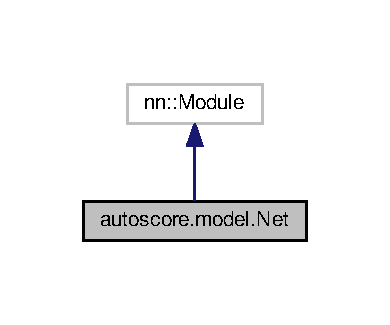
\includegraphics[width=187pt]{classautoscore_1_1model_1_1Net__inherit__graph}
\end{center}
\end{figure}


Collaboration diagram for autoscore.\+model.\+Net\+:\nopagebreak
\begin{figure}[H]
\begin{center}
\leavevmode
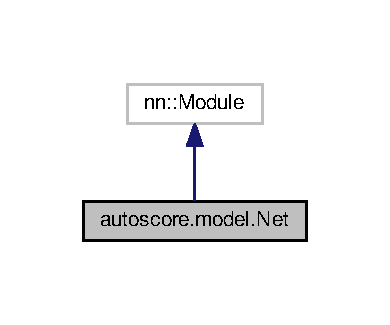
\includegraphics[width=187pt]{classautoscore_1_1model_1_1Net__coll__graph}
\end{center}
\end{figure}
\subsection*{Public Member Functions}
\begin{DoxyCompactItemize}
\item 
def \hyperlink{classautoscore_1_1model_1_1Net_a25b2d2e182c0444ef17ac2528a9395d8}{\+\_\+\+\_\+init\+\_\+\+\_\+} (self)
\item 
def \hyperlink{classautoscore_1_1model_1_1Net_a21c71ff3dd5f3fbbc0c3f5a28500ac41}{forward} (self, x)
\end{DoxyCompactItemize}
\subsection*{Public Attributes}
\begin{DoxyCompactItemize}
\item 
\hyperlink{classautoscore_1_1model_1_1Net_a627695d95db2a994bef69b3a89c51c30}{conv1}
\item 
\hyperlink{classautoscore_1_1model_1_1Net_a1c3f9d3b681c1f611c28a818c18f70e6}{conv2}
\item 
\hyperlink{classautoscore_1_1model_1_1Net_aea9cd230e23281abf4d8d23e768b7918}{conv2\+\_\+drop}
\item 
\hyperlink{classautoscore_1_1model_1_1Net_ace16e109006254bbd976660c4df63ac8}{fc1}
\item 
\hyperlink{classautoscore_1_1model_1_1Net_ac2913be42e89e170ae4829f901169e46}{fc2}
\end{DoxyCompactItemize}


\subsection{Detailed Description}


Definition at line 9 of file model.\+py.



\subsection{Constructor \& Destructor Documentation}
\index{autoscore\+::model\+::\+Net@{autoscore\+::model\+::\+Net}!\+\_\+\+\_\+init\+\_\+\+\_\+@{\+\_\+\+\_\+init\+\_\+\+\_\+}}
\index{\+\_\+\+\_\+init\+\_\+\+\_\+@{\+\_\+\+\_\+init\+\_\+\+\_\+}!autoscore\+::model\+::\+Net@{autoscore\+::model\+::\+Net}}
\subsubsection[{\texorpdfstring{\+\_\+\+\_\+init\+\_\+\+\_\+(self)}{__init__(self)}}]{\setlength{\rightskip}{0pt plus 5cm}def autoscore.\+model.\+Net.\+\_\+\+\_\+init\+\_\+\+\_\+ (
\begin{DoxyParamCaption}
\item[{}]{self}
\end{DoxyParamCaption}
)}\hypertarget{classautoscore_1_1model_1_1Net_a25b2d2e182c0444ef17ac2528a9395d8}{}\label{classautoscore_1_1model_1_1Net_a25b2d2e182c0444ef17ac2528a9395d8}


Definition at line 10 of file model.\+py.



\subsection{Member Function Documentation}
\index{autoscore\+::model\+::\+Net@{autoscore\+::model\+::\+Net}!forward@{forward}}
\index{forward@{forward}!autoscore\+::model\+::\+Net@{autoscore\+::model\+::\+Net}}
\subsubsection[{\texorpdfstring{forward(self, x)}{forward(self, x)}}]{\setlength{\rightskip}{0pt plus 5cm}def autoscore.\+model.\+Net.\+forward (
\begin{DoxyParamCaption}
\item[{}]{self, }
\item[{}]{x}
\end{DoxyParamCaption}
)}\hypertarget{classautoscore_1_1model_1_1Net_a21c71ff3dd5f3fbbc0c3f5a28500ac41}{}\label{classautoscore_1_1model_1_1Net_a21c71ff3dd5f3fbbc0c3f5a28500ac41}


Definition at line 18 of file model.\+py.



\subsection{Member Data Documentation}
\index{autoscore\+::model\+::\+Net@{autoscore\+::model\+::\+Net}!conv1@{conv1}}
\index{conv1@{conv1}!autoscore\+::model\+::\+Net@{autoscore\+::model\+::\+Net}}
\subsubsection[{\texorpdfstring{conv1}{conv1}}]{\setlength{\rightskip}{0pt plus 5cm}autoscore.\+model.\+Net.\+conv1}\hypertarget{classautoscore_1_1model_1_1Net_a627695d95db2a994bef69b3a89c51c30}{}\label{classautoscore_1_1model_1_1Net_a627695d95db2a994bef69b3a89c51c30}


Definition at line 12 of file model.\+py.

\index{autoscore\+::model\+::\+Net@{autoscore\+::model\+::\+Net}!conv2@{conv2}}
\index{conv2@{conv2}!autoscore\+::model\+::\+Net@{autoscore\+::model\+::\+Net}}
\subsubsection[{\texorpdfstring{conv2}{conv2}}]{\setlength{\rightskip}{0pt plus 5cm}autoscore.\+model.\+Net.\+conv2}\hypertarget{classautoscore_1_1model_1_1Net_a1c3f9d3b681c1f611c28a818c18f70e6}{}\label{classautoscore_1_1model_1_1Net_a1c3f9d3b681c1f611c28a818c18f70e6}


Definition at line 13 of file model.\+py.

\index{autoscore\+::model\+::\+Net@{autoscore\+::model\+::\+Net}!conv2\+\_\+drop@{conv2\+\_\+drop}}
\index{conv2\+\_\+drop@{conv2\+\_\+drop}!autoscore\+::model\+::\+Net@{autoscore\+::model\+::\+Net}}
\subsubsection[{\texorpdfstring{conv2\+\_\+drop}{conv2_drop}}]{\setlength{\rightskip}{0pt plus 5cm}autoscore.\+model.\+Net.\+conv2\+\_\+drop}\hypertarget{classautoscore_1_1model_1_1Net_aea9cd230e23281abf4d8d23e768b7918}{}\label{classautoscore_1_1model_1_1Net_aea9cd230e23281abf4d8d23e768b7918}


Definition at line 14 of file model.\+py.

\index{autoscore\+::model\+::\+Net@{autoscore\+::model\+::\+Net}!fc1@{fc1}}
\index{fc1@{fc1}!autoscore\+::model\+::\+Net@{autoscore\+::model\+::\+Net}}
\subsubsection[{\texorpdfstring{fc1}{fc1}}]{\setlength{\rightskip}{0pt plus 5cm}autoscore.\+model.\+Net.\+fc1}\hypertarget{classautoscore_1_1model_1_1Net_ace16e109006254bbd976660c4df63ac8}{}\label{classautoscore_1_1model_1_1Net_ace16e109006254bbd976660c4df63ac8}


Definition at line 15 of file model.\+py.

\index{autoscore\+::model\+::\+Net@{autoscore\+::model\+::\+Net}!fc2@{fc2}}
\index{fc2@{fc2}!autoscore\+::model\+::\+Net@{autoscore\+::model\+::\+Net}}
\subsubsection[{\texorpdfstring{fc2}{fc2}}]{\setlength{\rightskip}{0pt plus 5cm}autoscore.\+model.\+Net.\+fc2}\hypertarget{classautoscore_1_1model_1_1Net_ac2913be42e89e170ae4829f901169e46}{}\label{classautoscore_1_1model_1_1Net_ac2913be42e89e170ae4829f901169e46}


Definition at line 16 of file model.\+py.



The documentation for this class was generated from the following file\+:\begin{DoxyCompactItemize}
\item 
src/autoscore/\hyperlink{model_8py}{model.\+py}\end{DoxyCompactItemize}

\hypertarget{structanonymous__namespace_02staff_8cc_03_1_1RunLengthData}{}\section{anonymous\+\_\+namespace\{staff.\+cc\}\+:\+:Run\+Length\+Data Struct Reference}
\label{structanonymous__namespace_02staff_8cc_03_1_1RunLengthData}\index{anonymous\+\_\+namespace\lcurly{}staff.\+cc\rcurly{}\+::\+Run\+Length\+Data@{anonymous\+\_\+namespace\lcurly{}staff.\+cc\rcurly{}\+::\+Run\+Length\+Data}}
\subsection*{Public Attributes}
\begin{DoxyCompactItemize}
\item 
cv\+::\+Mat \hyperlink{structanonymous__namespace_02staff_8cc_03_1_1RunLengthData_a5e1faf2a25c952ac51297388a44af198}{img}
\item 
std\+::vector$<$ int $>$ $\ast$ \hyperlink{structanonymous__namespace_02staff_8cc_03_1_1RunLengthData_a3ed6930a2e526ce64cccba0e86ac8c29}{whites}
\item 
std\+::vector$<$ int $>$ $\ast$ \hyperlink{structanonymous__namespace_02staff_8cc_03_1_1RunLengthData_acac0ba1ce364389ce57220db37036035}{blacks}
\item 
int \hyperlink{structanonymous__namespace_02staff_8cc_03_1_1RunLengthData_a74e9de2cf82afdb5754a7ec5b6c15817}{start}
\item 
int \hyperlink{structanonymous__namespace_02staff_8cc_03_1_1RunLengthData_a4eb4c72887a7a75f3b99c711a7af9638}{finish}
\end{DoxyCompactItemize}


\subsection{Detailed Description}


Definition at line 154 of file staff.\+cc.



\subsection{Member Data Documentation}
\index{anonymous\+\_\+namespace\lcurly{}staff.\+cc\rcurly{}\+::\+Run\+Length\+Data@{anonymous\+\_\+namespace\lcurly{}staff.\+cc\rcurly{}\+::\+Run\+Length\+Data}!blacks@{blacks}}
\index{blacks@{blacks}!anonymous\+\_\+namespace\lcurly{}staff.\+cc\rcurly{}\+::\+Run\+Length\+Data@{anonymous\+\_\+namespace\lcurly{}staff.\+cc\rcurly{}\+::\+Run\+Length\+Data}}
\subsubsection[{\texorpdfstring{blacks}{blacks}}]{\setlength{\rightskip}{0pt plus 5cm}std\+::vector$<$int$>$ $\ast$ anonymous\+\_\+namespace\{staff.\+cc\}\+::Run\+Length\+Data\+::blacks}\hypertarget{structanonymous__namespace_02staff_8cc_03_1_1RunLengthData_acac0ba1ce364389ce57220db37036035}{}\label{structanonymous__namespace_02staff_8cc_03_1_1RunLengthData_acac0ba1ce364389ce57220db37036035}


Definition at line 156 of file staff.\+cc.

\index{anonymous\+\_\+namespace\lcurly{}staff.\+cc\rcurly{}\+::\+Run\+Length\+Data@{anonymous\+\_\+namespace\lcurly{}staff.\+cc\rcurly{}\+::\+Run\+Length\+Data}!finish@{finish}}
\index{finish@{finish}!anonymous\+\_\+namespace\lcurly{}staff.\+cc\rcurly{}\+::\+Run\+Length\+Data@{anonymous\+\_\+namespace\lcurly{}staff.\+cc\rcurly{}\+::\+Run\+Length\+Data}}
\subsubsection[{\texorpdfstring{finish}{finish}}]{\setlength{\rightskip}{0pt plus 5cm}int anonymous\+\_\+namespace\{staff.\+cc\}\+::Run\+Length\+Data\+::finish}\hypertarget{structanonymous__namespace_02staff_8cc_03_1_1RunLengthData_a4eb4c72887a7a75f3b99c711a7af9638}{}\label{structanonymous__namespace_02staff_8cc_03_1_1RunLengthData_a4eb4c72887a7a75f3b99c711a7af9638}


Definition at line 157 of file staff.\+cc.

\index{anonymous\+\_\+namespace\lcurly{}staff.\+cc\rcurly{}\+::\+Run\+Length\+Data@{anonymous\+\_\+namespace\lcurly{}staff.\+cc\rcurly{}\+::\+Run\+Length\+Data}!img@{img}}
\index{img@{img}!anonymous\+\_\+namespace\lcurly{}staff.\+cc\rcurly{}\+::\+Run\+Length\+Data@{anonymous\+\_\+namespace\lcurly{}staff.\+cc\rcurly{}\+::\+Run\+Length\+Data}}
\subsubsection[{\texorpdfstring{img}{img}}]{\setlength{\rightskip}{0pt plus 5cm}cv\+::\+Mat anonymous\+\_\+namespace\{staff.\+cc\}\+::Run\+Length\+Data\+::img}\hypertarget{structanonymous__namespace_02staff_8cc_03_1_1RunLengthData_a5e1faf2a25c952ac51297388a44af198}{}\label{structanonymous__namespace_02staff_8cc_03_1_1RunLengthData_a5e1faf2a25c952ac51297388a44af198}


Definition at line 155 of file staff.\+cc.

\index{anonymous\+\_\+namespace\lcurly{}staff.\+cc\rcurly{}\+::\+Run\+Length\+Data@{anonymous\+\_\+namespace\lcurly{}staff.\+cc\rcurly{}\+::\+Run\+Length\+Data}!start@{start}}
\index{start@{start}!anonymous\+\_\+namespace\lcurly{}staff.\+cc\rcurly{}\+::\+Run\+Length\+Data@{anonymous\+\_\+namespace\lcurly{}staff.\+cc\rcurly{}\+::\+Run\+Length\+Data}}
\subsubsection[{\texorpdfstring{start}{start}}]{\setlength{\rightskip}{0pt plus 5cm}int anonymous\+\_\+namespace\{staff.\+cc\}\+::Run\+Length\+Data\+::start}\hypertarget{structanonymous__namespace_02staff_8cc_03_1_1RunLengthData_a74e9de2cf82afdb5754a7ec5b6c15817}{}\label{structanonymous__namespace_02staff_8cc_03_1_1RunLengthData_a74e9de2cf82afdb5754a7ec5b6c15817}


Definition at line 157 of file staff.\+cc.

\index{anonymous\+\_\+namespace\lcurly{}staff.\+cc\rcurly{}\+::\+Run\+Length\+Data@{anonymous\+\_\+namespace\lcurly{}staff.\+cc\rcurly{}\+::\+Run\+Length\+Data}!whites@{whites}}
\index{whites@{whites}!anonymous\+\_\+namespace\lcurly{}staff.\+cc\rcurly{}\+::\+Run\+Length\+Data@{anonymous\+\_\+namespace\lcurly{}staff.\+cc\rcurly{}\+::\+Run\+Length\+Data}}
\subsubsection[{\texorpdfstring{whites}{whites}}]{\setlength{\rightskip}{0pt plus 5cm}std\+::vector$<$int$>$$\ast$ anonymous\+\_\+namespace\{staff.\+cc\}\+::Run\+Length\+Data\+::whites}\hypertarget{structanonymous__namespace_02staff_8cc_03_1_1RunLengthData_a3ed6930a2e526ce64cccba0e86ac8c29}{}\label{structanonymous__namespace_02staff_8cc_03_1_1RunLengthData_a3ed6930a2e526ce64cccba0e86ac8c29}


Definition at line 156 of file staff.\+cc.



The documentation for this struct was generated from the following file\+:\begin{DoxyCompactItemize}
\item 
src/autoscore/\hyperlink{staff_8cc}{staff.\+cc}\end{DoxyCompactItemize}

\hypertarget{structStaffModel}{}\section{Staff\+Model Struct Reference}
\label{structStaffModel}\index{Staff\+Model@{Staff\+Model}}


\hyperlink{structStaffModel}{Staff\+Model} that holds the gradient (or orientation) at each column.  




{\ttfamily \#include $<$staff.\+hh$>$}

\subsection*{Public Attributes}
\begin{DoxyCompactItemize}
\item 
std\+::vector$<$ double $>$ \hyperlink{structStaffModel_a2c7b2b9d75456613e3543ccf9538ca94}{gradient}
\item 
int \hyperlink{structStaffModel_a0d40c0261502458fa794f81f7a39ffef}{start\+\_\+col}
\item 
int \hyperlink{structStaffModel_a116b56bb5fb2a12531ea020a5c93f9a7}{start\+\_\+row}
\item 
int \hyperlink{structStaffModel_a4bc9a16b2d5cdd2ba93926e2f208acf7}{staff\+\_\+height}
\item 
int \hyperlink{structStaffModel_a64ddccbd4d416dba382ae9f4f9bbe7fc}{staff\+\_\+space}
\item 
double \hyperlink{structStaffModel_aa887f6067d99543cc6ffaa237f19ef87}{rot}
\item 
bool \hyperlink{structStaffModel_aa3c9a53c181ac34279101f3aaa15f1e6}{straight}
\item 
cv\+::\+Mat \hyperlink{structStaffModel_a52f39a8c36879ed8e536fe6e3f89aeb7}{staff\+\_\+image}
\end{DoxyCompactItemize}


\subsection{Detailed Description}
\hyperlink{structStaffModel}{Staff\+Model} that holds the gradient (or orientation) at each column. 

Definition at line 10 of file staff.\+hh.



\subsection{Member Data Documentation}
\index{Staff\+Model@{Staff\+Model}!gradient@{gradient}}
\index{gradient@{gradient}!Staff\+Model@{Staff\+Model}}
\subsubsection[{\texorpdfstring{gradient}{gradient}}]{\setlength{\rightskip}{0pt plus 5cm}std\+::vector$<$double$>$ Staff\+Model\+::gradient}\hypertarget{structStaffModel_a2c7b2b9d75456613e3543ccf9538ca94}{}\label{structStaffModel_a2c7b2b9d75456613e3543ccf9538ca94}


Definition at line 11 of file staff.\+hh.

\index{Staff\+Model@{Staff\+Model}!rot@{rot}}
\index{rot@{rot}!Staff\+Model@{Staff\+Model}}
\subsubsection[{\texorpdfstring{rot}{rot}}]{\setlength{\rightskip}{0pt plus 5cm}double Staff\+Model\+::rot}\hypertarget{structStaffModel_aa887f6067d99543cc6ffaa237f19ef87}{}\label{structStaffModel_aa887f6067d99543cc6ffaa237f19ef87}


Definition at line 13 of file staff.\+hh.

\index{Staff\+Model@{Staff\+Model}!staff\+\_\+height@{staff\+\_\+height}}
\index{staff\+\_\+height@{staff\+\_\+height}!Staff\+Model@{Staff\+Model}}
\subsubsection[{\texorpdfstring{staff\+\_\+height}{staff_height}}]{\setlength{\rightskip}{0pt plus 5cm}int Staff\+Model\+::staff\+\_\+height}\hypertarget{structStaffModel_a4bc9a16b2d5cdd2ba93926e2f208acf7}{}\label{structStaffModel_a4bc9a16b2d5cdd2ba93926e2f208acf7}


Definition at line 12 of file staff.\+hh.

\index{Staff\+Model@{Staff\+Model}!staff\+\_\+image@{staff\+\_\+image}}
\index{staff\+\_\+image@{staff\+\_\+image}!Staff\+Model@{Staff\+Model}}
\subsubsection[{\texorpdfstring{staff\+\_\+image}{staff_image}}]{\setlength{\rightskip}{0pt plus 5cm}cv\+::\+Mat Staff\+Model\+::staff\+\_\+image}\hypertarget{structStaffModel_a52f39a8c36879ed8e536fe6e3f89aeb7}{}\label{structStaffModel_a52f39a8c36879ed8e536fe6e3f89aeb7}


Definition at line 15 of file staff.\+hh.

\index{Staff\+Model@{Staff\+Model}!staff\+\_\+space@{staff\+\_\+space}}
\index{staff\+\_\+space@{staff\+\_\+space}!Staff\+Model@{Staff\+Model}}
\subsubsection[{\texorpdfstring{staff\+\_\+space}{staff_space}}]{\setlength{\rightskip}{0pt plus 5cm}int Staff\+Model\+::staff\+\_\+space}\hypertarget{structStaffModel_a64ddccbd4d416dba382ae9f4f9bbe7fc}{}\label{structStaffModel_a64ddccbd4d416dba382ae9f4f9bbe7fc}


Definition at line 12 of file staff.\+hh.

\index{Staff\+Model@{Staff\+Model}!start\+\_\+col@{start\+\_\+col}}
\index{start\+\_\+col@{start\+\_\+col}!Staff\+Model@{Staff\+Model}}
\subsubsection[{\texorpdfstring{start\+\_\+col}{start_col}}]{\setlength{\rightskip}{0pt plus 5cm}int Staff\+Model\+::start\+\_\+col}\hypertarget{structStaffModel_a0d40c0261502458fa794f81f7a39ffef}{}\label{structStaffModel_a0d40c0261502458fa794f81f7a39ffef}


Definition at line 12 of file staff.\+hh.

\index{Staff\+Model@{Staff\+Model}!start\+\_\+row@{start\+\_\+row}}
\index{start\+\_\+row@{start\+\_\+row}!Staff\+Model@{Staff\+Model}}
\subsubsection[{\texorpdfstring{start\+\_\+row}{start_row}}]{\setlength{\rightskip}{0pt plus 5cm}int Staff\+Model\+::start\+\_\+row}\hypertarget{structStaffModel_a116b56bb5fb2a12531ea020a5c93f9a7}{}\label{structStaffModel_a116b56bb5fb2a12531ea020a5c93f9a7}


Definition at line 12 of file staff.\+hh.

\index{Staff\+Model@{Staff\+Model}!straight@{straight}}
\index{straight@{straight}!Staff\+Model@{Staff\+Model}}
\subsubsection[{\texorpdfstring{straight}{straight}}]{\setlength{\rightskip}{0pt plus 5cm}bool Staff\+Model\+::straight}\hypertarget{structStaffModel_aa3c9a53c181ac34279101f3aaa15f1e6}{}\label{structStaffModel_aa3c9a53c181ac34279101f3aaa15f1e6}


Definition at line 14 of file staff.\+hh.



The documentation for this struct was generated from the following file\+:\begin{DoxyCompactItemize}
\item 
include/autoscore/\hyperlink{staff_8hh}{staff.\+hh}\end{DoxyCompactItemize}

\chapter{File Documentation}
\hypertarget{staff_8hh}{}\section{include/autoscore/staff.hh File Reference}
\label{staff_8hh}\index{include/autoscore/staff.\+hh@{include/autoscore/staff.\+hh}}
{\ttfamily \#include $<$opencv2/opencv.\+hpp$>$}\\*
{\ttfamily \#include $<$vector$>$}\\*
Include dependency graph for staff.\+hh\+:\nopagebreak
\begin{figure}[H]
\begin{center}
\leavevmode
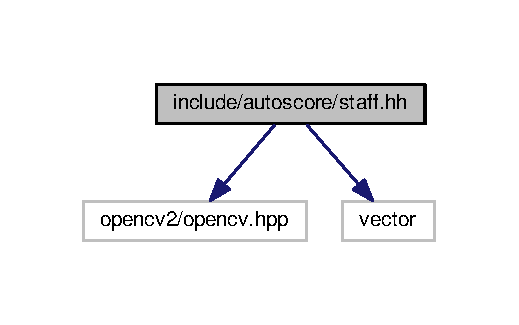
\includegraphics[width=249pt]{staff_8hh__incl}
\end{center}
\end{figure}
This graph shows which files directly or indirectly include this file\+:\nopagebreak
\begin{figure}[H]
\begin{center}
\leavevmode
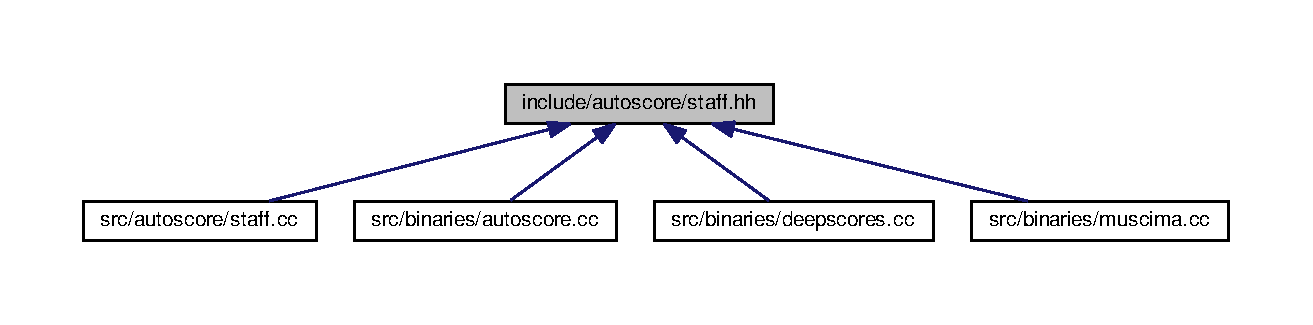
\includegraphics[width=350pt]{staff_8hh__dep__incl}
\end{center}
\end{figure}
\subsection*{Classes}
\begin{DoxyCompactItemize}
\item 
struct \hyperlink{structStaffModel}{Staff\+Model}
\begin{DoxyCompactList}\small\item\em \hyperlink{structStaffModel}{Staff\+Model} that holds the gradient (or orientation) at each column. \end{DoxyCompactList}\end{DoxyCompactItemize}
\subsection*{Namespaces}
\begin{DoxyCompactItemize}
\item 
 \hyperlink{namespaceas}{as}
\item 
 \hyperlink{namespaceas_1_1staff}{as\+::staff}
\end{DoxyCompactItemize}
\subsection*{Typedefs}
\begin{DoxyCompactItemize}
\item 
typedef std\+::vector$<$ std\+::pair$<$ int, int $>$ $>$ \hyperlink{staff_8hh_acfffa1dd2bf9ce5820435e63446a7c90}{Staffs}
\begin{DoxyCompactList}\small\item\em Vector of staffs with first and last line. Combined with a staff model, it can serve pitch inference. \end{DoxyCompactList}\end{DoxyCompactItemize}
\subsection*{Functions}
\begin{DoxyCompactItemize}
\item 
\hyperlink{structStaffModel}{Staff\+Model} \hyperlink{namespaceas_1_1staff_adc528d054888cbe3b9da25286da8aef6}{as\+::staff\+::\+Get\+Staff\+Model} (const cv\+::\+Mat \&src, const int n\+\_\+threads=1)
\begin{DoxyCompactList}\small\item\em Estimates a staff model from a binary image. \end{DoxyCompactList}\item 
void \hyperlink{namespaceas_1_1staff_a9c48cfcf1c17cad08ed233fe90d05839}{as\+::staff\+::\+Print\+Staff\+Model} (cv\+::\+Mat \&dst, const \hyperlink{structStaffModel}{Staff\+Model} \&model)
\begin{DoxyCompactList}\small\item\em Prints a staff model on a black image. \end{DoxyCompactList}\item 
\hyperlink{staff_8hh_acfffa1dd2bf9ce5820435e63446a7c90}{Staffs} \hyperlink{namespaceas_1_1staff_a8a53d0c0106d677e72ae36edb5bbd760}{as\+::staff\+::\+Fit\+Staff\+Model} (const \hyperlink{structStaffModel}{Staff\+Model} \&model)
\begin{DoxyCompactList}\small\item\em Fits the given model and returns all valid staffs. \end{DoxyCompactList}\item 
void \hyperlink{namespaceas_1_1staff_a5209861cdb891c8a12b5ef43784fac77}{as\+::staff\+::\+Print\+Staffs} (cv\+::\+Mat \&dst, const \hyperlink{staff_8hh_acfffa1dd2bf9ce5820435e63446a7c90}{Staffs} \&staffs, const \hyperlink{structStaffModel}{Staff\+Model} \&model)
\begin{DoxyCompactList}\small\item\em Prints all the detected staffs of the model on an image. \end{DoxyCompactList}\item 
void \hyperlink{namespaceas_1_1staff_ae06eef6c527f2a2919cc8344394fc80c}{as\+::staff\+::\+Remove\+Staffs} (cv\+::\+Mat \&dst, const \hyperlink{staff_8hh_acfffa1dd2bf9ce5820435e63446a7c90}{Staffs} \&staffs, const \hyperlink{structStaffModel}{Staff\+Model} \&model)
\begin{DoxyCompactList}\small\item\em Removes staffs from an image according to a model and start and end positions. \end{DoxyCompactList}\item 
void \hyperlink{namespaceas_1_1staff_af93180a3091e6494dc9983792c5113dc}{as\+::staff\+::\+Realign} (cv\+::\+Mat \&dst, const \hyperlink{structStaffModel}{Staff\+Model} \&model)
\begin{DoxyCompactList}\small\item\em Realigns the image according to the staff model gradient. The output image is then modeled with a constant gradient. To distort back the image, give the inverse of the model ($\ast$-\/1). \end{DoxyCompactList}\item 
void \hyperlink{namespaceas_1_1staff_a568fd337876db996340be89931a8b908}{as\+::staff\+::\+Save\+To\+Disk} (const std\+::string \&fn, const \hyperlink{staff_8hh_acfffa1dd2bf9ce5820435e63446a7c90}{Staffs} \&staffs, const \hyperlink{structStaffModel}{Staff\+Model} \&model)
\begin{DoxyCompactList}\small\item\em Saves the staff information in a xml format. \end{DoxyCompactList}\end{DoxyCompactItemize}


\subsection{Typedef Documentation}
\index{staff.\+hh@{staff.\+hh}!Staffs@{Staffs}}
\index{Staffs@{Staffs}!staff.\+hh@{staff.\+hh}}
\subsubsection[{\texorpdfstring{Staffs}{Staffs}}]{\setlength{\rightskip}{0pt plus 5cm}typedef std\+::vector$<$std\+::pair$<$int, int$>$ $>$ {\bf Staffs}}\hypertarget{staff_8hh_acfffa1dd2bf9ce5820435e63446a7c90}{}\label{staff_8hh_acfffa1dd2bf9ce5820435e63446a7c90}


Vector of staffs with first and last line. Combined with a staff model, it can serve pitch inference. 



Definition at line 22 of file staff.\+hh.


\hypertarget{util_8hh}{}\section{include/autoscore/util.hh File Reference}
\label{util_8hh}\index{include/autoscore/util.\+hh@{include/autoscore/util.\+hh}}
{\ttfamily \#include $<$string$>$}\\*
Include dependency graph for util.\+hh\+:\nopagebreak
\begin{figure}[H]
\begin{center}
\leavevmode
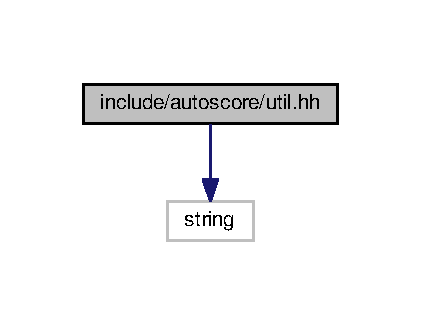
\includegraphics[width=202pt]{util_8hh__incl}
\end{center}
\end{figure}
This graph shows which files directly or indirectly include this file\+:\nopagebreak
\begin{figure}[H]
\begin{center}
\leavevmode
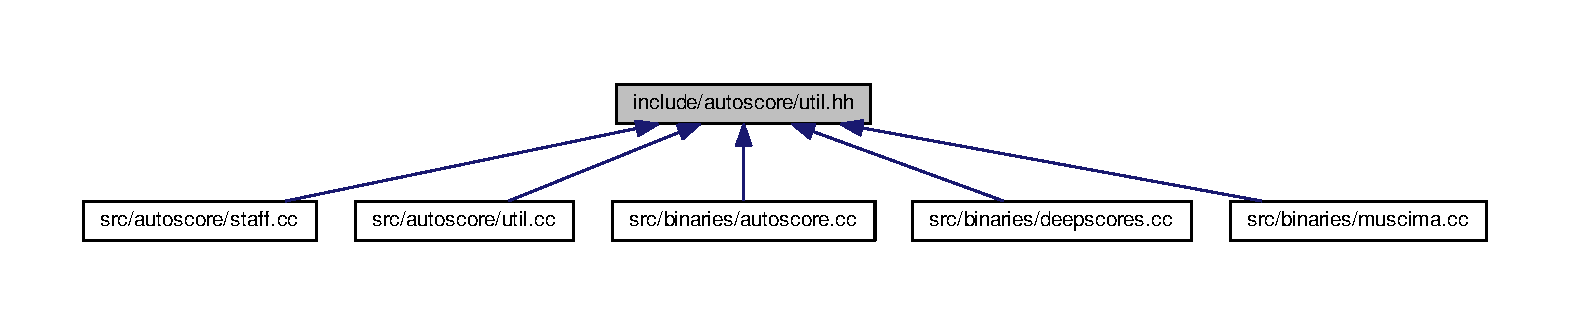
\includegraphics[width=350pt]{util_8hh__dep__incl}
\end{center}
\end{figure}
\subsection*{Functions}
\begin{DoxyCompactItemize}
\item 
std\+::string \hyperlink{util_8hh_ae5b4e4cefa23bc996fed995252867396}{strip\+\_\+fn} (const std\+::string \&fn)
\begin{DoxyCompactList}\small\item\em Strips the path of a filename. \end{DoxyCompactList}\item 
std\+::string \hyperlink{util_8hh_ae6b89cc6e7775692353c55bf356bbac1}{strip\+\_\+ext} (const std\+::string \&fn)
\begin{DoxyCompactList}\small\item\em Strips the extension of a file. \end{DoxyCompactList}\item 
bool \hyperlink{util_8hh_a273d906b424684c9d83f3ec3ac3be35a}{is\+\_\+image} (const std\+::string \&fn)
\begin{DoxyCompactList}\small\item\em Checks if the filename is an image supported by Open\+CV. \end{DoxyCompactList}\end{DoxyCompactItemize}


\subsection{Function Documentation}
\index{util.\+hh@{util.\+hh}!is\+\_\+image@{is\+\_\+image}}
\index{is\+\_\+image@{is\+\_\+image}!util.\+hh@{util.\+hh}}
\subsubsection[{\texorpdfstring{is\+\_\+image(const std\+::string \&fn)}{is_image(const std::string &fn)}}]{\setlength{\rightskip}{0pt plus 5cm}bool is\+\_\+image (
\begin{DoxyParamCaption}
\item[{const std\+::string \&}]{fn}
\end{DoxyParamCaption}
)\hspace{0.3cm}{\ttfamily [inline]}}\hypertarget{util_8hh_a273d906b424684c9d83f3ec3ac3be35a}{}\label{util_8hh_a273d906b424684c9d83f3ec3ac3be35a}


Checks if the filename is an image supported by Open\+CV. 


\begin{DoxyParams}{Parameters}
{\em fn} & The filename \\
\hline
\end{DoxyParams}
\begin{DoxyReturn}{Returns}
Whether or not the filename is a valid image 
\end{DoxyReturn}


Definition at line 28 of file util.\+hh.

\index{util.\+hh@{util.\+hh}!strip\+\_\+ext@{strip\+\_\+ext}}
\index{strip\+\_\+ext@{strip\+\_\+ext}!util.\+hh@{util.\+hh}}
\subsubsection[{\texorpdfstring{strip\+\_\+ext(const std\+::string \&fn)}{strip_ext(const std::string &fn)}}]{\setlength{\rightskip}{0pt plus 5cm}std\+::string strip\+\_\+ext (
\begin{DoxyParamCaption}
\item[{const std\+::string \&}]{fn}
\end{DoxyParamCaption}
)}\hypertarget{util_8hh_ae6b89cc6e7775692353c55bf356bbac1}{}\label{util_8hh_ae6b89cc6e7775692353c55bf356bbac1}


Strips the extension of a file. 


\begin{DoxyParams}{Parameters}
{\em fn} & Path to the file \\
\hline
\end{DoxyParams}
\begin{DoxyReturn}{Returns}
Path without the extension 
\end{DoxyReturn}


Definition at line 18 of file util.\+cc.

\index{util.\+hh@{util.\+hh}!strip\+\_\+fn@{strip\+\_\+fn}}
\index{strip\+\_\+fn@{strip\+\_\+fn}!util.\+hh@{util.\+hh}}
\subsubsection[{\texorpdfstring{strip\+\_\+fn(const std\+::string \&fn)}{strip_fn(const std::string &fn)}}]{\setlength{\rightskip}{0pt plus 5cm}std\+::string strip\+\_\+fn (
\begin{DoxyParamCaption}
\item[{const std\+::string \&}]{fn}
\end{DoxyParamCaption}
)}\hypertarget{util_8hh_ae5b4e4cefa23bc996fed995252867396}{}\label{util_8hh_ae5b4e4cefa23bc996fed995252867396}


Strips the path of a filename. 


\begin{DoxyParams}{Parameters}
{\em fn} & Absolute or relative filename \\
\hline
\end{DoxyParams}
\begin{DoxyReturn}{Returns}
Name of the file 
\end{DoxyReturn}


Definition at line 3 of file util.\+cc.


\hypertarget{____init_____8py}{}\section{src/autoscore/\+\_\+\+\_\+init\+\_\+\+\_\+.py File Reference}
\label{____init_____8py}\index{src/autoscore/\+\_\+\+\_\+init\+\_\+\+\_\+.\+py@{src/autoscore/\+\_\+\+\_\+init\+\_\+\+\_\+.\+py}}
\subsection*{Namespaces}
\begin{DoxyCompactItemize}
\item 
 \hyperlink{namespaceautoscore}{autoscore}
\end{DoxyCompactItemize}

\hypertarget{model_8py}{}\section{src/autoscore/model.py File Reference}
\label{model_8py}\index{src/autoscore/model.\+py@{src/autoscore/model.\+py}}
\subsection*{Classes}
\begin{DoxyCompactItemize}
\item 
class \hyperlink{classautoscore_1_1model_1_1Net}{autoscore.\+model.\+Net}
\end{DoxyCompactItemize}
\subsection*{Namespaces}
\begin{DoxyCompactItemize}
\item 
 \hyperlink{namespaceautoscore_1_1model}{autoscore.\+model}
\end{DoxyCompactItemize}
\subsection*{Functions}
\begin{DoxyCompactItemize}
\item 
def \hyperlink{namespaceautoscore_1_1model_a51ffe01b340b5e803be4afb24e44b482}{autoscore.\+model.\+train} (args, model, device, train\+\_\+loader, optimizer, epoch)
\item 
def \hyperlink{namespaceautoscore_1_1model_a224f5bb7be0a0950973797af8127c73e}{autoscore.\+model.\+test} (args, model, device, test\+\_\+loader)
\item 
def \hyperlink{namespaceautoscore_1_1model_a5207a743d3b33b8901a1139dea14b35f}{autoscore.\+model.\+main} ()
\end{DoxyCompactItemize}

\hypertarget{musicdata_8py}{}\section{src/autoscore/musicdata.py File Reference}
\label{musicdata_8py}\index{src/autoscore/musicdata.\+py@{src/autoscore/musicdata.\+py}}
\subsection*{Classes}
\begin{DoxyCompactItemize}
\item 
class \hyperlink{classautoscore_1_1musicdata_1_1MusicFile}{autoscore.\+musicdata.\+Music\+File}
\end{DoxyCompactItemize}
\subsection*{Namespaces}
\begin{DoxyCompactItemize}
\item 
 \hyperlink{namespaceautoscore_1_1musicdata}{autoscore.\+musicdata}
\end{DoxyCompactItemize}
\subsection*{Functions}
\begin{DoxyCompactItemize}
\item 
def \hyperlink{namespaceautoscore_1_1musicdata_a36b9f5fe5a2cb7a9d515e6d31108d71a}{autoscore.\+musicdata.\+\_\+setup\+\_\+dir} ()
\item 
def \hyperlink{namespaceautoscore_1_1musicdata_a680b60ad4d68bf01c129bce2ed53ed13}{autoscore.\+musicdata.\+get\+\_\+deepscores\+\_\+data} (images\+\_\+dir, gt\+\_\+dir)
\item 
def \hyperlink{namespaceautoscore_1_1musicdata_a4cc1edc9297b14e64c6824bfc80391be}{autoscore.\+musicdata.\+get\+\_\+muscima\+\_\+data} (images\+\_\+dir, gt\+\_\+dir)
\item 
def \hyperlink{namespaceautoscore_1_1musicdata_aeaaa4a2e6a03894586dd145faf0be207}{autoscore.\+musicdata.\+cross\+\_\+section} (first\+\_\+coordinates, second\+\_\+coordinates)
\item 
def \hyperlink{namespaceautoscore_1_1musicdata_af800c02302b00cd70bc8d82a349f2c34}{autoscore.\+musicdata.\+get\+\_\+music\+\_\+file\+\_\+from\+\_\+xml} (fn)
\item 
def \hyperlink{namespaceautoscore_1_1musicdata_a74762dd30814e9d65c87c0d9f16895d9}{autoscore.\+musicdata.\+deepscores\+\_\+score\+\_\+ground\+\_\+truth} (score\+\_\+filename, dataset\+\_\+filename)
\item 
def \hyperlink{namespaceautoscore_1_1musicdata_ab473d740a7364fed122ad806ff33651c}{autoscore.\+musicdata.\+muscima\+\_\+score\+\_\+ground\+\_\+truth} (score\+\_\+filename, dataset\+\_\+filename)
\item 
def \hyperlink{namespaceautoscore_1_1musicdata_af4a4d05f09aeaa84bb9014d40d0c0309}{autoscore.\+musicdata.\+sort\+\_\+by\+\_\+writers} (music\+\_\+files)
\end{DoxyCompactItemize}
\subsection*{Variables}
\begin{DoxyCompactItemize}
\item 
string \hyperlink{namespaceautoscore_1_1musicdata_a684ad72261f10358480f889b7c755716}{autoscore.\+musicdata.\+P\+R\+E\+F\+I\+X\+\_\+\+FN} = expanduser(\char`\"{}$\sim$\char`\"{})+\textquotesingle{}/Documents/auto-\/score/\textquotesingle{}
\item 
string \hyperlink{namespaceautoscore_1_1musicdata_acfb5d195ffef1d88681f6e3555219925}{autoscore.\+musicdata.\+A\+R\+T\+I\+F\+I\+C\+I\+A\+L\+\_\+\+FN} = P\+R\+E\+F\+I\+X\+\_\+\+FN+\textquotesingle{}datasets/Artificial/\textquotesingle{}
\item 
string \hyperlink{namespaceautoscore_1_1musicdata_af9a3c9c8a04c4a8459cff06c8d91a202}{autoscore.\+musicdata.\+H\+A\+N\+D\+W\+R\+I\+T\+T\+E\+N\+\_\+\+FN} = P\+R\+E\+F\+I\+X\+\_\+\+FN+\textquotesingle{}datasets/Handwritten/\textquotesingle{}
\item 
string \hyperlink{namespaceautoscore_1_1musicdata_a6e0e7fa09f8f4907ed2774f39c417c8d}{autoscore.\+musicdata.\+A\+R\+T\+I\+F\+I\+C\+I\+A\+L\+\_\+\+F\+N\+\_\+\+X\+ML} = A\+R\+T\+I\+F\+I\+C\+I\+A\+L\+\_\+\+FN+\textquotesingle{}xml/\textquotesingle{}
\item 
string \hyperlink{namespaceautoscore_1_1musicdata_a10c11cab7fc783ad0b9185fc95581f59}{autoscore.\+musicdata.\+H\+A\+N\+D\+W\+R\+I\+T\+T\+E\+N\+\_\+\+F\+N\+\_\+\+X\+ML} = H\+A\+N\+D\+W\+R\+I\+T\+T\+E\+N\+\_\+\+FN+\textquotesingle{}xml/\textquotesingle{}
\item 
string \hyperlink{namespaceautoscore_1_1musicdata_a47cc3f7854416092969250879a8a0d7f}{autoscore.\+musicdata.\+A\+R\+T\+I\+F\+I\+C\+I\+A\+L\+\_\+\+F\+N\+\_\+\+D\+A\+TA} = A\+R\+T\+I\+F\+I\+C\+I\+A\+L\+\_\+\+FN+\textquotesingle{}data/\textquotesingle{}
\item 
string \hyperlink{namespaceautoscore_1_1musicdata_a323dfa7bb6acca22309294f911611ce1}{autoscore.\+musicdata.\+H\+A\+N\+D\+W\+R\+I\+T\+T\+E\+N\+\_\+\+F\+N\+\_\+\+D\+A\+TA} = H\+A\+N\+D\+W\+R\+I\+T\+T\+E\+N\+\_\+\+FN+\textquotesingle{}data/\textquotesingle{}
\item 
\hyperlink{namespaceautoscore_1_1musicdata_a54a64afd77bd1565c3680deb249d3d6a}{autoscore.\+musicdata.\+Glyph} = namedtuple(\textquotesingle{}Glyph\textquotesingle{}, \textquotesingle{}name bbox\textquotesingle{})
\item 
\hyperlink{namespaceautoscore_1_1musicdata_a0c7624e21c2d8b4557c7552671a2e538}{autoscore.\+musicdata.\+B\+Box} = namedtuple(\textquotesingle{}Bbox\textquotesingle{}, \textquotesingle{}xmin xmax ymin ymax\textquotesingle{})
\item 
float \hyperlink{namespaceautoscore_1_1musicdata_abf4865a17c78985e607f4f7e2b9f5e62}{autoscore.\+musicdata.\+S\+T\+R\+I\+D\+E\+\_\+\+R\+A\+T\+IO} = 0.\+5
\item 
int \hyperlink{namespaceautoscore_1_1musicdata_a5b8b64595027a20c59f8323de8526e30}{autoscore.\+musicdata.\+B\+O\+U\+N\+D\+A\+R\+Y\+\_\+\+E\+X\+T\+RA} = 4
\item 
int \hyperlink{namespaceautoscore_1_1musicdata_a4342208695b0441e76d13ad639c1d700}{autoscore.\+musicdata.\+P\+O\+L\+L\+\_\+\+T\+H\+R\+E\+SH} = 50
\item 
int \hyperlink{namespaceautoscore_1_1musicdata_a355d8fb1a4b75793b64381e7097d51b7}{autoscore.\+musicdata.\+E\+P\+S\+I\+L\+ON} = 1
\item 
float \hyperlink{namespaceautoscore_1_1musicdata_aa2545f5fe006ee17a14f604063447c90}{autoscore.\+musicdata.\+A\+R\+E\+A\+\_\+\+O\+V\+E\+R\+L\+A\+P\+\_\+\+M\+IN} = 0.\+6
\item 
int \hyperlink{namespaceautoscore_1_1musicdata_a8bdc2ab9668f34c2e203c42365bf9047}{autoscore.\+musicdata.\+R\+ED} = 255
\item 
int \hyperlink{namespaceautoscore_1_1musicdata_a7373305dc96aaa767d13d24287c70269}{autoscore.\+musicdata.\+B\+L\+UE} = 0
\item 
int \hyperlink{namespaceautoscore_1_1musicdata_af0a6b998fc1cb73188462d6dc9dc9719}{autoscore.\+musicdata.\+G\+R\+E\+EN} = 0
\item 
dictionary \hyperlink{namespaceautoscore_1_1musicdata_a2d30a65a367d3fd398938b3d45c9dcab}{autoscore.\+musicdata.\+R\+E\+L\+E\+V\+A\+N\+T\+\_\+\+G\+L\+Y\+P\+HS}
\end{DoxyCompactItemize}

\hypertarget{staff_8cc}{}\section{src/autoscore/staff.cc File Reference}
\label{staff_8cc}\index{src/autoscore/staff.\+cc@{src/autoscore/staff.\+cc}}
{\ttfamily \#include $<$autoscore/staff.\+hh$>$}\\*
{\ttfamily \#include $<$autoscore/util.\+hh$>$}\\*
{\ttfamily \#include $<$tinyxml2.\+hh$>$}\\*
{\ttfamily \#include $<$map$>$}\\*
{\ttfamily \#include $<$thread$>$}\\*
{\ttfamily \#include $<$assert.\+h$>$}\\*
{\ttfamily \#include $<$unistd.\+h$>$}\\*
Include dependency graph for staff.\+cc\+:
\nopagebreak
\begin{figure}[H]
\begin{center}
\leavevmode
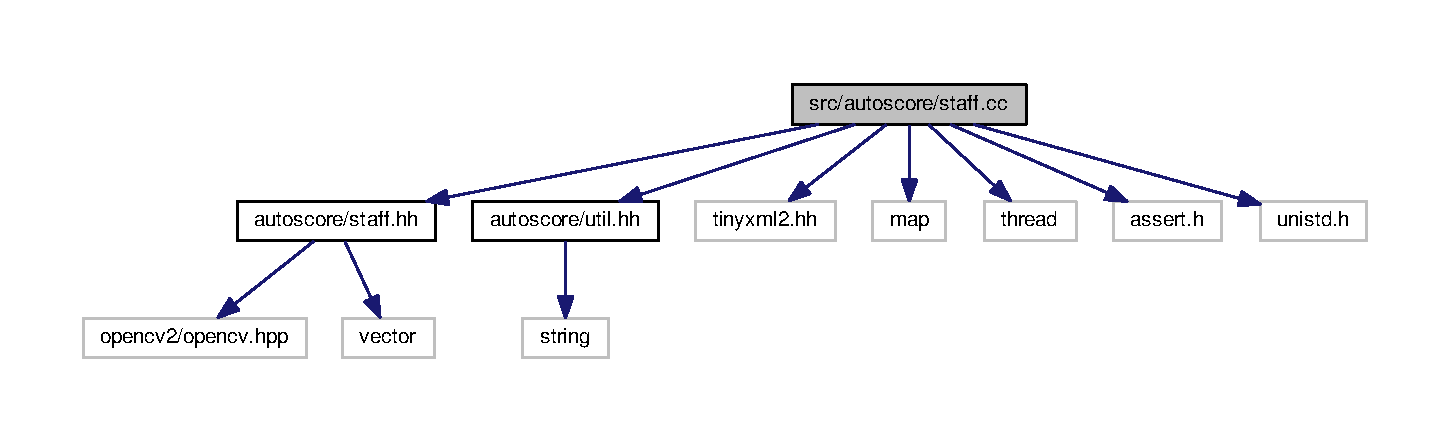
\includegraphics[width=350pt]{staff_8cc__incl}
\end{center}
\end{figure}
\subsection*{Classes}
\begin{DoxyCompactItemize}
\item 
struct \hyperlink{structanonymous__namespace_02staff_8cc_03_1_1RunLengthData}{anonymous\+\_\+namespace\{staff.\+cc\}\+::\+Run\+Length\+Data}
\item 
struct \hyperlink{structanonymous__namespace_02staff_8cc_03_1_1ConnectedComponent}{anonymous\+\_\+namespace\{staff.\+cc\}\+::\+Connected\+Component}
\item 
struct \hyperlink{structanonymous__namespace_02staff_8cc_03_1_1GradientData}{anonymous\+\_\+namespace\{staff.\+cc\}\+::\+Gradient\+Data}
\end{DoxyCompactItemize}
\subsection*{Namespaces}
\begin{DoxyCompactItemize}
\item 
 \hyperlink{namespaceanonymous__namespace_02staff_8cc_03}{anonymous\+\_\+namespace\{staff.\+cc\}}
\end{DoxyCompactItemize}
\subsection*{Macros}
\begin{DoxyCompactItemize}
\item 
\#define \hyperlink{staff_8cc_abf72175efb60132ac964e52aeb5f7c83}{B\+I\+N\+A\+R\+Y\+\_\+\+T\+H\+R\+E\+S\+H\+\_\+\+V\+AL}~128
\item 
\#define \hyperlink{staff_8cc_a76d59f8c36ada225964995e650db5b66}{M\+I\+N\+\_\+\+C\+O\+N\+N\+E\+C\+T\+E\+D\+\_\+\+C\+O\+MP}~10
\item 
\#define \hyperlink{staff_8cc_a88674420e534cbc53dd6a0a435b78df3}{K\+\_\+\+N\+E\+A\+R\+E\+ST}~5
\item 
\#define \hyperlink{staff_8cc_aae9a32fb4ed60a2b23dd7eca52e8e627}{K\+E\+R\+N\+E\+L\+\_\+\+S\+I\+ZE}~5
\item 
\#define \hyperlink{staff_8cc_ad4bd7dadb8ed3df5ec153534ad54ba94}{M\+I\+N\+\_\+\+P\+O\+L\+L\+\_\+\+P\+E\+R\+\_\+\+L\+I\+N\+E\+\_\+\+R\+A\+T\+IO}~0.\+75
\item 
\#define \hyperlink{staff_8cc_af9842f4040a0b015b015a7c7804adeff}{P\+O\+L\+L\+\_\+\+P\+E\+R\+\_\+\+S\+T\+A\+F\+F\+\_\+\+R\+A\+T\+IO}~0.\+6
\item 
\#define \hyperlink{staff_8cc_a7e54beaa2e3b43b0200ddb1cd5a3f8f0}{M\+I\+N\+\_\+\+H\+O\+U\+G\+H\+\_\+\+L\+I\+N\+ES}~10
\item 
\#define \hyperlink{staff_8cc_accb87656b6abb5b7cb82f10bd6e91ec4}{T\+H\+E\+T\+A\+\_\+\+R\+ES}~2
\item 
\#define \hyperlink{staff_8cc_a401f1cca6f833dfa7601f22db5431067}{N\+\_\+\+B\+I\+NS}~20
\item 
\#define \hyperlink{staff_8cc_af189f6fc2ab90b54e5551679f0385ff0}{L\+I\+N\+E\+S\+\_\+\+P\+E\+R\+\_\+\+S\+T\+A\+FF}~5
\item 
\#define \hyperlink{staff_8cc_ac5a945020d3528355cda82d383676736}{R\+A\+D2\+D\+EG}~180 / C\+V\+\_\+\+PI
\item 
\#define \hyperlink{staff_8cc_af7e8592d0a634bd3642e9fd508ea8022}{D\+E\+G2\+R\+AD}~1 / (\hyperlink{staff_8cc_ac5a945020d3528355cda82d383676736}{R\+A\+D2\+D\+EG})
\item 
\#define \hyperlink{staff_8cc_a002b2f4894492820fe708b1b7e7c5e70}{E\+P\+S\+I\+L\+ON}~1e-\/7
\end{DoxyCompactItemize}
\subsection*{Functions}
\begin{DoxyCompactItemize}
\item 
bool \hyperlink{namespaceanonymous__namespace_02staff_8cc_03_a79495cf4f6a32aa51f293ed70e818804}{anonymous\+\_\+namespace\{staff.\+cc\}\+::is\+\_\+gray} (const cv\+::\+Mat \&src)
\item 
void \hyperlink{namespaceanonymous__namespace_02staff_8cc_03_a57d06804211d80274cc40825db82bfcb}{anonymous\+\_\+namespace\{staff.\+cc\}\+::bounding\+\_\+box} (const cv\+::\+Mat \&src, cv\+::\+Mat \&dst)
\item 
void \hyperlink{namespaceanonymous__namespace_02staff_8cc_03_a3568b86a70e0f8a3daec31a019eeb104}{anonymous\+\_\+namespace\{staff.\+cc\}\+::draw\+\_\+model} (cv\+::\+Mat \&dst, const \hyperlink{structStaffModel}{Staff\+Model} \&model, const int pos, const cv\+::\+Scalar color)
\item 
void \hyperlink{namespaceanonymous__namespace_02staff_8cc_03_a9156ea35902498bfb94f9f22b8f4bf6e}{anonymous\+\_\+namespace\{staff.\+cc\}\+::rotate\+\_\+image} (cv\+::\+Mat \&dst, const double rot\+\_\+theta)
\item 
void \hyperlink{namespaceanonymous__namespace_02staff_8cc_03_a5bdda2981a95b5eb6d486efc14676724}{anonymous\+\_\+namespace\{staff.\+cc\}\+::raw\+\_\+rotate} (cv\+::\+Mat \&dst, const double rot\+\_\+theta)
\item 
bool \hyperlink{namespaceanonymous__namespace_02staff_8cc_03_a63818cc0df79b80ab6ffcad5b63df63a}{anonymous\+\_\+namespace\{staff.\+cc\}\+::black\+\_\+on\+\_\+white} (const cv\+::\+Mat \&src)
\item 
void \hyperlink{namespaceanonymous__namespace_02staff_8cc_03_a6e1c8cba88d76c900e8c838e6e97beb8}{anonymous\+\_\+namespace\{staff.\+cc\}\+::estimate\+\_\+rotation} (cv\+::\+Mat \&img, \hyperlink{structStaffModel}{Staff\+Model} \&model)
\item 
void \hyperlink{namespaceanonymous__namespace_02staff_8cc_03_ab0f140df81f62c7aa0f330a0a876b5cf}{anonymous\+\_\+namespace\{staff.\+cc\}\+::run\+\_\+length\+\_\+p} (struct Run\+Length\+Data \&data)
\item 
void \hyperlink{namespaceanonymous__namespace_02staff_8cc_03_afe2c1f1f40fd4b176293cdc981bdd6b9}{anonymous\+\_\+namespace\{staff.\+cc\}\+::run\+\_\+length} (const cv\+::\+Mat \&img, int \&staff\+\_\+height, int \&staff\+\_\+space, const int n\+\_\+threads)
\item 
void \hyperlink{namespaceanonymous__namespace_02staff_8cc_03_a88b9ddc21068ab319b4e4366abb95a8b}{anonymous\+\_\+namespace\{staff.\+cc\}\+::remove\+\_\+glyphs} (cv\+::\+Mat \&staff\+\_\+image, const int staff\+\_\+height, const int staff\+\_\+space)
\item 
void \hyperlink{namespaceanonymous__namespace_02staff_8cc_03_af9ad599266f45cfd7cbd4108a1d15927}{anonymous\+\_\+namespace\{staff.\+cc\}\+::estimate\+\_\+gradient\+\_\+p} (struct Gradient\+Data \&data)
\item 
void \hyperlink{namespaceanonymous__namespace_02staff_8cc_03_ab397b0436cc25a1d1b61be4bd5be3c35}{anonymous\+\_\+namespace\{staff.\+cc\}\+::estimate\+\_\+gradient} (\hyperlink{structStaffModel}{Staff\+Model} \&model, const int n\+\_\+threads)
\item 
void \hyperlink{namespaceanonymous__namespace_02staff_8cc_03_a5f56c8cd80f73838161c63d79eee1e80}{anonymous\+\_\+namespace\{staff.\+cc\}\+::interpolate\+\_\+model} (\hyperlink{structStaffModel}{Staff\+Model} \&model)
\item 
std\+::vector$<$ int $>$ \hyperlink{namespaceanonymous__namespace_02staff_8cc_03_ab179502b6b6aa0bbe43936bac2f43411}{anonymous\+\_\+namespace\{staff.\+cc\}\+::poll\+\_\+lines} (const \hyperlink{structStaffModel}{Staff\+Model} \&model)
\item 
void \hyperlink{namespaceanonymous__namespace_02staff_8cc_03_a0a9d89aad47af23fc68cfb5600c4eb98}{anonymous\+\_\+namespace\{staff.\+cc\}\+::remove\+\_\+line} (cv\+::\+Mat \&dst, double line\+\_\+pos, const \hyperlink{structStaffModel}{Staff\+Model} \&model)
\end{DoxyCompactItemize}


\subsection{Macro Definition Documentation}
\index{staff.\+cc@{staff.\+cc}!B\+I\+N\+A\+R\+Y\+\_\+\+T\+H\+R\+E\+S\+H\+\_\+\+V\+AL@{B\+I\+N\+A\+R\+Y\+\_\+\+T\+H\+R\+E\+S\+H\+\_\+\+V\+AL}}
\index{B\+I\+N\+A\+R\+Y\+\_\+\+T\+H\+R\+E\+S\+H\+\_\+\+V\+AL@{B\+I\+N\+A\+R\+Y\+\_\+\+T\+H\+R\+E\+S\+H\+\_\+\+V\+AL}!staff.\+cc@{staff.\+cc}}
\subsubsection[{\texorpdfstring{B\+I\+N\+A\+R\+Y\+\_\+\+T\+H\+R\+E\+S\+H\+\_\+\+V\+AL}{BINARY_THRESH_VAL}}]{\setlength{\rightskip}{0pt plus 5cm}\#define B\+I\+N\+A\+R\+Y\+\_\+\+T\+H\+R\+E\+S\+H\+\_\+\+V\+AL~128}\hypertarget{staff_8cc_abf72175efb60132ac964e52aeb5f7c83}{}\label{staff_8cc_abf72175efb60132ac964e52aeb5f7c83}


Definition at line 14 of file staff.\+cc.

\index{staff.\+cc@{staff.\+cc}!D\+E\+G2\+R\+AD@{D\+E\+G2\+R\+AD}}
\index{D\+E\+G2\+R\+AD@{D\+E\+G2\+R\+AD}!staff.\+cc@{staff.\+cc}}
\subsubsection[{\texorpdfstring{D\+E\+G2\+R\+AD}{DEG2RAD}}]{\setlength{\rightskip}{0pt plus 5cm}\#define D\+E\+G2\+R\+AD~1 / ({\bf R\+A\+D2\+D\+EG})}\hypertarget{staff_8cc_af7e8592d0a634bd3642e9fd508ea8022}{}\label{staff_8cc_af7e8592d0a634bd3642e9fd508ea8022}


Definition at line 35 of file staff.\+cc.

\index{staff.\+cc@{staff.\+cc}!E\+P\+S\+I\+L\+ON@{E\+P\+S\+I\+L\+ON}}
\index{E\+P\+S\+I\+L\+ON@{E\+P\+S\+I\+L\+ON}!staff.\+cc@{staff.\+cc}}
\subsubsection[{\texorpdfstring{E\+P\+S\+I\+L\+ON}{EPSILON}}]{\setlength{\rightskip}{0pt plus 5cm}\#define E\+P\+S\+I\+L\+ON~1e-\/7}\hypertarget{staff_8cc_a002b2f4894492820fe708b1b7e7c5e70}{}\label{staff_8cc_a002b2f4894492820fe708b1b7e7c5e70}


Definition at line 36 of file staff.\+cc.

\index{staff.\+cc@{staff.\+cc}!K\+\_\+\+N\+E\+A\+R\+E\+ST@{K\+\_\+\+N\+E\+A\+R\+E\+ST}}
\index{K\+\_\+\+N\+E\+A\+R\+E\+ST@{K\+\_\+\+N\+E\+A\+R\+E\+ST}!staff.\+cc@{staff.\+cc}}
\subsubsection[{\texorpdfstring{K\+\_\+\+N\+E\+A\+R\+E\+ST}{K_NEAREST}}]{\setlength{\rightskip}{0pt plus 5cm}\#define K\+\_\+\+N\+E\+A\+R\+E\+ST~5}\hypertarget{staff_8cc_a88674420e534cbc53dd6a0a435b78df3}{}\label{staff_8cc_a88674420e534cbc53dd6a0a435b78df3}


Definition at line 18 of file staff.\+cc.

\index{staff.\+cc@{staff.\+cc}!K\+E\+R\+N\+E\+L\+\_\+\+S\+I\+ZE@{K\+E\+R\+N\+E\+L\+\_\+\+S\+I\+ZE}}
\index{K\+E\+R\+N\+E\+L\+\_\+\+S\+I\+ZE@{K\+E\+R\+N\+E\+L\+\_\+\+S\+I\+ZE}!staff.\+cc@{staff.\+cc}}
\subsubsection[{\texorpdfstring{K\+E\+R\+N\+E\+L\+\_\+\+S\+I\+ZE}{KERNEL_SIZE}}]{\setlength{\rightskip}{0pt plus 5cm}\#define K\+E\+R\+N\+E\+L\+\_\+\+S\+I\+ZE~5}\hypertarget{staff_8cc_aae9a32fb4ed60a2b23dd7eca52e8e627}{}\label{staff_8cc_aae9a32fb4ed60a2b23dd7eca52e8e627}


Definition at line 20 of file staff.\+cc.

\index{staff.\+cc@{staff.\+cc}!L\+I\+N\+E\+S\+\_\+\+P\+E\+R\+\_\+\+S\+T\+A\+FF@{L\+I\+N\+E\+S\+\_\+\+P\+E\+R\+\_\+\+S\+T\+A\+FF}}
\index{L\+I\+N\+E\+S\+\_\+\+P\+E\+R\+\_\+\+S\+T\+A\+FF@{L\+I\+N\+E\+S\+\_\+\+P\+E\+R\+\_\+\+S\+T\+A\+FF}!staff.\+cc@{staff.\+cc}}
\subsubsection[{\texorpdfstring{L\+I\+N\+E\+S\+\_\+\+P\+E\+R\+\_\+\+S\+T\+A\+FF}{LINES_PER_STAFF}}]{\setlength{\rightskip}{0pt plus 5cm}\#define L\+I\+N\+E\+S\+\_\+\+P\+E\+R\+\_\+\+S\+T\+A\+FF~5}\hypertarget{staff_8cc_af189f6fc2ab90b54e5551679f0385ff0}{}\label{staff_8cc_af189f6fc2ab90b54e5551679f0385ff0}


Definition at line 33 of file staff.\+cc.

\index{staff.\+cc@{staff.\+cc}!M\+I\+N\+\_\+\+C\+O\+N\+N\+E\+C\+T\+E\+D\+\_\+\+C\+O\+MP@{M\+I\+N\+\_\+\+C\+O\+N\+N\+E\+C\+T\+E\+D\+\_\+\+C\+O\+MP}}
\index{M\+I\+N\+\_\+\+C\+O\+N\+N\+E\+C\+T\+E\+D\+\_\+\+C\+O\+MP@{M\+I\+N\+\_\+\+C\+O\+N\+N\+E\+C\+T\+E\+D\+\_\+\+C\+O\+MP}!staff.\+cc@{staff.\+cc}}
\subsubsection[{\texorpdfstring{M\+I\+N\+\_\+\+C\+O\+N\+N\+E\+C\+T\+E\+D\+\_\+\+C\+O\+MP}{MIN_CONNECTED_COMP}}]{\setlength{\rightskip}{0pt plus 5cm}\#define M\+I\+N\+\_\+\+C\+O\+N\+N\+E\+C\+T\+E\+D\+\_\+\+C\+O\+MP~10}\hypertarget{staff_8cc_a76d59f8c36ada225964995e650db5b66}{}\label{staff_8cc_a76d59f8c36ada225964995e650db5b66}


Definition at line 16 of file staff.\+cc.

\index{staff.\+cc@{staff.\+cc}!M\+I\+N\+\_\+\+H\+O\+U\+G\+H\+\_\+\+L\+I\+N\+ES@{M\+I\+N\+\_\+\+H\+O\+U\+G\+H\+\_\+\+L\+I\+N\+ES}}
\index{M\+I\+N\+\_\+\+H\+O\+U\+G\+H\+\_\+\+L\+I\+N\+ES@{M\+I\+N\+\_\+\+H\+O\+U\+G\+H\+\_\+\+L\+I\+N\+ES}!staff.\+cc@{staff.\+cc}}
\subsubsection[{\texorpdfstring{M\+I\+N\+\_\+\+H\+O\+U\+G\+H\+\_\+\+L\+I\+N\+ES}{MIN_HOUGH_LINES}}]{\setlength{\rightskip}{0pt plus 5cm}\#define M\+I\+N\+\_\+\+H\+O\+U\+G\+H\+\_\+\+L\+I\+N\+ES~10}\hypertarget{staff_8cc_a7e54beaa2e3b43b0200ddb1cd5a3f8f0}{}\label{staff_8cc_a7e54beaa2e3b43b0200ddb1cd5a3f8f0}


Definition at line 26 of file staff.\+cc.

\index{staff.\+cc@{staff.\+cc}!M\+I\+N\+\_\+\+P\+O\+L\+L\+\_\+\+P\+E\+R\+\_\+\+L\+I\+N\+E\+\_\+\+R\+A\+T\+IO@{M\+I\+N\+\_\+\+P\+O\+L\+L\+\_\+\+P\+E\+R\+\_\+\+L\+I\+N\+E\+\_\+\+R\+A\+T\+IO}}
\index{M\+I\+N\+\_\+\+P\+O\+L\+L\+\_\+\+P\+E\+R\+\_\+\+L\+I\+N\+E\+\_\+\+R\+A\+T\+IO@{M\+I\+N\+\_\+\+P\+O\+L\+L\+\_\+\+P\+E\+R\+\_\+\+L\+I\+N\+E\+\_\+\+R\+A\+T\+IO}!staff.\+cc@{staff.\+cc}}
\subsubsection[{\texorpdfstring{M\+I\+N\+\_\+\+P\+O\+L\+L\+\_\+\+P\+E\+R\+\_\+\+L\+I\+N\+E\+\_\+\+R\+A\+T\+IO}{MIN_POLL_PER_LINE_RATIO}}]{\setlength{\rightskip}{0pt plus 5cm}\#define M\+I\+N\+\_\+\+P\+O\+L\+L\+\_\+\+P\+E\+R\+\_\+\+L\+I\+N\+E\+\_\+\+R\+A\+T\+IO~0.\+75}\hypertarget{staff_8cc_ad4bd7dadb8ed3df5ec153534ad54ba94}{}\label{staff_8cc_ad4bd7dadb8ed3df5ec153534ad54ba94}


Definition at line 22 of file staff.\+cc.

\index{staff.\+cc@{staff.\+cc}!N\+\_\+\+B\+I\+NS@{N\+\_\+\+B\+I\+NS}}
\index{N\+\_\+\+B\+I\+NS@{N\+\_\+\+B\+I\+NS}!staff.\+cc@{staff.\+cc}}
\subsubsection[{\texorpdfstring{N\+\_\+\+B\+I\+NS}{N_BINS}}]{\setlength{\rightskip}{0pt plus 5cm}\#define N\+\_\+\+B\+I\+NS~20}\hypertarget{staff_8cc_a401f1cca6f833dfa7601f22db5431067}{}\label{staff_8cc_a401f1cca6f833dfa7601f22db5431067}


Definition at line 30 of file staff.\+cc.

\index{staff.\+cc@{staff.\+cc}!P\+O\+L\+L\+\_\+\+P\+E\+R\+\_\+\+S\+T\+A\+F\+F\+\_\+\+R\+A\+T\+IO@{P\+O\+L\+L\+\_\+\+P\+E\+R\+\_\+\+S\+T\+A\+F\+F\+\_\+\+R\+A\+T\+IO}}
\index{P\+O\+L\+L\+\_\+\+P\+E\+R\+\_\+\+S\+T\+A\+F\+F\+\_\+\+R\+A\+T\+IO@{P\+O\+L\+L\+\_\+\+P\+E\+R\+\_\+\+S\+T\+A\+F\+F\+\_\+\+R\+A\+T\+IO}!staff.\+cc@{staff.\+cc}}
\subsubsection[{\texorpdfstring{P\+O\+L\+L\+\_\+\+P\+E\+R\+\_\+\+S\+T\+A\+F\+F\+\_\+\+R\+A\+T\+IO}{POLL_PER_STAFF_RATIO}}]{\setlength{\rightskip}{0pt plus 5cm}\#define P\+O\+L\+L\+\_\+\+P\+E\+R\+\_\+\+S\+T\+A\+F\+F\+\_\+\+R\+A\+T\+IO~0.\+6}\hypertarget{staff_8cc_af9842f4040a0b015b015a7c7804adeff}{}\label{staff_8cc_af9842f4040a0b015b015a7c7804adeff}


Definition at line 24 of file staff.\+cc.

\index{staff.\+cc@{staff.\+cc}!R\+A\+D2\+D\+EG@{R\+A\+D2\+D\+EG}}
\index{R\+A\+D2\+D\+EG@{R\+A\+D2\+D\+EG}!staff.\+cc@{staff.\+cc}}
\subsubsection[{\texorpdfstring{R\+A\+D2\+D\+EG}{RAD2DEG}}]{\setlength{\rightskip}{0pt plus 5cm}\#define R\+A\+D2\+D\+EG~180 / C\+V\+\_\+\+PI}\hypertarget{staff_8cc_ac5a945020d3528355cda82d383676736}{}\label{staff_8cc_ac5a945020d3528355cda82d383676736}


Definition at line 34 of file staff.\+cc.

\index{staff.\+cc@{staff.\+cc}!T\+H\+E\+T\+A\+\_\+\+R\+ES@{T\+H\+E\+T\+A\+\_\+\+R\+ES}}
\index{T\+H\+E\+T\+A\+\_\+\+R\+ES@{T\+H\+E\+T\+A\+\_\+\+R\+ES}!staff.\+cc@{staff.\+cc}}
\subsubsection[{\texorpdfstring{T\+H\+E\+T\+A\+\_\+\+R\+ES}{THETA_RES}}]{\setlength{\rightskip}{0pt plus 5cm}\#define T\+H\+E\+T\+A\+\_\+\+R\+ES~2}\hypertarget{staff_8cc_accb87656b6abb5b7cb82f10bd6e91ec4}{}\label{staff_8cc_accb87656b6abb5b7cb82f10bd6e91ec4}


Definition at line 29 of file staff.\+cc.


\hypertarget{util_8cc}{}\section{src/autoscore/util.cc File Reference}
\label{util_8cc}\index{src/autoscore/util.\+cc@{src/autoscore/util.\+cc}}
{\ttfamily \#include $<$autoscore/util.\+hh$>$}\\*
Include dependency graph for util.\+cc\+:\nopagebreak
\begin{figure}[H]
\begin{center}
\leavevmode
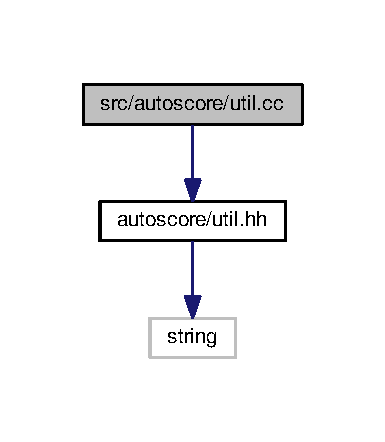
\includegraphics[width=185pt]{util_8cc__incl}
\end{center}
\end{figure}
\subsection*{Functions}
\begin{DoxyCompactItemize}
\item 
std\+::string \hyperlink{util_8cc_ae5b4e4cefa23bc996fed995252867396}{strip\+\_\+fn} (const std\+::string \&fn)
\begin{DoxyCompactList}\small\item\em Strips the path of a filename. \end{DoxyCompactList}\item 
std\+::string \hyperlink{util_8cc_ae6b89cc6e7775692353c55bf356bbac1}{strip\+\_\+ext} (const std\+::string \&fn)
\begin{DoxyCompactList}\small\item\em Strips the extension of a file. \end{DoxyCompactList}\end{DoxyCompactItemize}


\subsection{Function Documentation}
\index{util.\+cc@{util.\+cc}!strip\+\_\+ext@{strip\+\_\+ext}}
\index{strip\+\_\+ext@{strip\+\_\+ext}!util.\+cc@{util.\+cc}}
\subsubsection[{\texorpdfstring{strip\+\_\+ext(const std\+::string \&fn)}{strip_ext(const std::string &fn)}}]{\setlength{\rightskip}{0pt plus 5cm}std\+::string strip\+\_\+ext (
\begin{DoxyParamCaption}
\item[{const std\+::string \&}]{fn}
\end{DoxyParamCaption}
)}\hypertarget{util_8cc_ae6b89cc6e7775692353c55bf356bbac1}{}\label{util_8cc_ae6b89cc6e7775692353c55bf356bbac1}


Strips the extension of a file. 


\begin{DoxyParams}{Parameters}
{\em fn} & Path to the file \\
\hline
\end{DoxyParams}
\begin{DoxyReturn}{Returns}
Path without the extension 
\end{DoxyReturn}


Definition at line 18 of file util.\+cc.

\index{util.\+cc@{util.\+cc}!strip\+\_\+fn@{strip\+\_\+fn}}
\index{strip\+\_\+fn@{strip\+\_\+fn}!util.\+cc@{util.\+cc}}
\subsubsection[{\texorpdfstring{strip\+\_\+fn(const std\+::string \&fn)}{strip_fn(const std::string &fn)}}]{\setlength{\rightskip}{0pt plus 5cm}std\+::string strip\+\_\+fn (
\begin{DoxyParamCaption}
\item[{const std\+::string \&}]{fn}
\end{DoxyParamCaption}
)}\hypertarget{util_8cc_ae5b4e4cefa23bc996fed995252867396}{}\label{util_8cc_ae5b4e4cefa23bc996fed995252867396}


Strips the path of a filename. 


\begin{DoxyParams}{Parameters}
{\em fn} & Absolute or relative filename \\
\hline
\end{DoxyParams}
\begin{DoxyReturn}{Returns}
Name of the file 
\end{DoxyReturn}


Definition at line 3 of file util.\+cc.


\hypertarget{autoscore_8cc}{}\section{src/binaries/autoscore.cc File Reference}
\label{autoscore_8cc}\index{src/binaries/autoscore.\+cc@{src/binaries/autoscore.\+cc}}
{\ttfamily \#include $<$autoscore/staff.\+hh$>$}\\*
{\ttfamily \#include $<$autoscore/util.\+hh$>$}\\*
{\ttfamily \#include $<$opencv2/opencv.\+hpp$>$}\\*
{\ttfamily \#include $<$experimental/filesystem$>$}\\*
{\ttfamily \#include $<$string$>$}\\*
Include dependency graph for autoscore.\+cc\+:\nopagebreak
\begin{figure}[H]
\begin{center}
\leavevmode
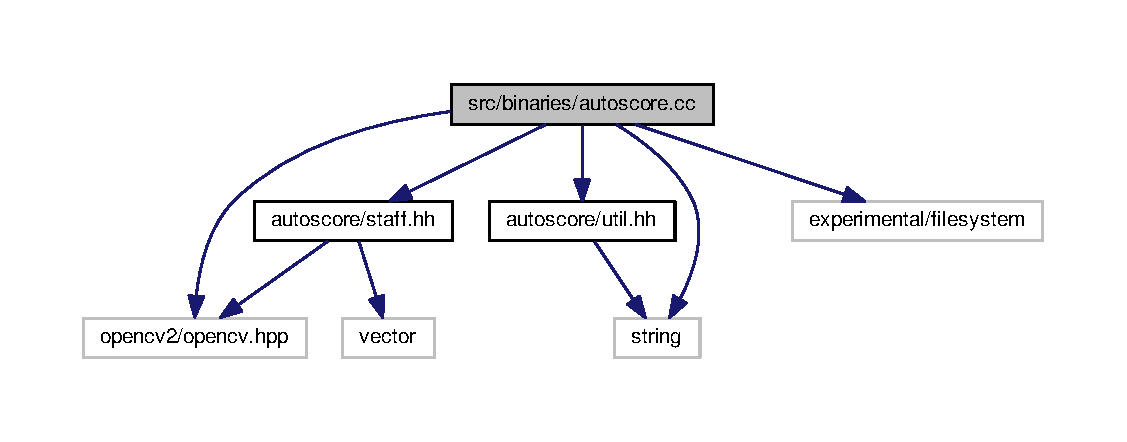
\includegraphics[width=350pt]{autoscore_8cc__incl}
\end{center}
\end{figure}
\subsection*{Functions}
\begin{DoxyCompactItemize}
\item 
void \hyperlink{autoscore_8cc_a666818ed37d4c58f0479a01910fdd50a}{process\+\_\+image} (const std\+::string \&fn, const int n\+\_\+threads)
\item 
int \hyperlink{autoscore_8cc_a3c04138a5bfe5d72780bb7e82a18e627}{main} (int argc, char $\ast$$\ast$argv)
\end{DoxyCompactItemize}


\subsection{Function Documentation}
\index{autoscore.\+cc@{autoscore.\+cc}!main@{main}}
\index{main@{main}!autoscore.\+cc@{autoscore.\+cc}}
\subsubsection[{\texorpdfstring{main(int argc, char $\ast$$\ast$argv)}{main(int argc, char **argv)}}]{\setlength{\rightskip}{0pt plus 5cm}int main (
\begin{DoxyParamCaption}
\item[{int}]{argc, }
\item[{char $\ast$$\ast$}]{argv}
\end{DoxyParamCaption}
)}\hypertarget{autoscore_8cc_a3c04138a5bfe5d72780bb7e82a18e627}{}\label{autoscore_8cc_a3c04138a5bfe5d72780bb7e82a18e627}


Definition at line 26 of file autoscore.\+cc.

\index{autoscore.\+cc@{autoscore.\+cc}!process\+\_\+image@{process\+\_\+image}}
\index{process\+\_\+image@{process\+\_\+image}!autoscore.\+cc@{autoscore.\+cc}}
\subsubsection[{\texorpdfstring{process\+\_\+image(const std\+::string \&fn, const int n\+\_\+threads)}{process_image(const std::string &fn, const int n_threads)}}]{\setlength{\rightskip}{0pt plus 5cm}void process\+\_\+image (
\begin{DoxyParamCaption}
\item[{const std\+::string \&}]{fn, }
\item[{const int}]{n\+\_\+threads}
\end{DoxyParamCaption}
)}\hypertarget{autoscore_8cc_a666818ed37d4c58f0479a01910fdd50a}{}\label{autoscore_8cc_a666818ed37d4c58f0479a01910fdd50a}


Definition at line 17 of file autoscore.\+cc.


\hypertarget{deepscores_8cc}{}\section{src/binaries/deepscores.cc File Reference}
\label{deepscores_8cc}\index{src/binaries/deepscores.\+cc@{src/binaries/deepscores.\+cc}}
{\ttfamily \#include $<$assert.\+h$>$}\\*
{\ttfamily \#include $<$experimental/filesystem$>$}\\*
{\ttfamily \#include $<$map$>$}\\*
{\ttfamily \#include $<$string$>$}\\*
{\ttfamily \#include $<$thread$>$}\\*
{\ttfamily \#include $<$vector$>$}\\*
{\ttfamily \#include $<$autoscore/staff.\+hh$>$}\\*
{\ttfamily \#include $<$autoscore/util.\+hh$>$}\\*
Include dependency graph for deepscores.\+cc\+:\nopagebreak
\begin{figure}[H]
\begin{center}
\leavevmode
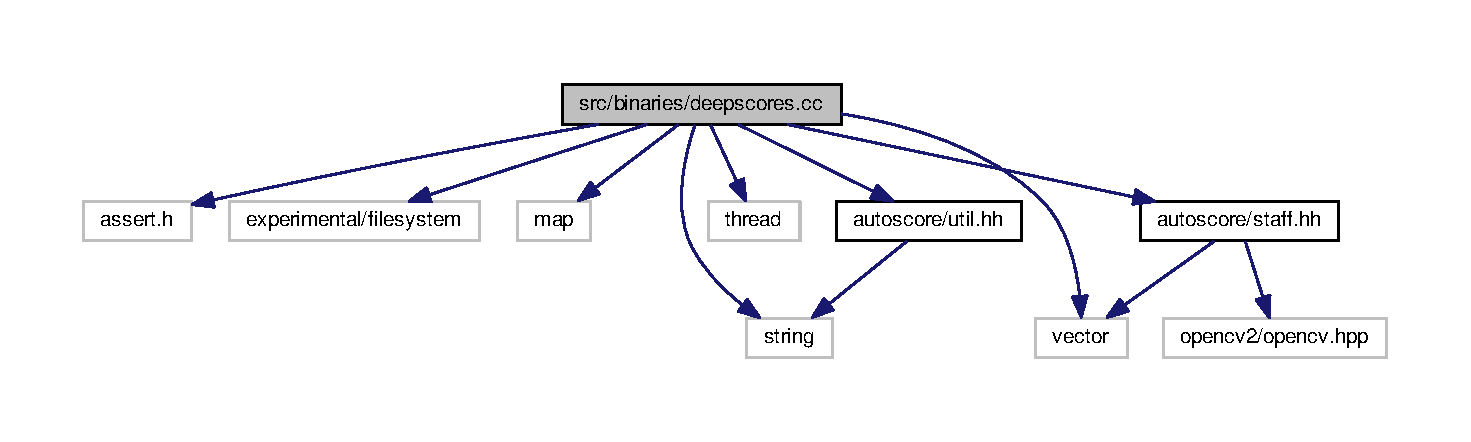
\includegraphics[width=350pt]{deepscores_8cc__incl}
\end{center}
\end{figure}
\subsection*{Macros}
\begin{DoxyCompactItemize}
\item 
\#define \hyperlink{deepscores_8cc_a1f08b99bca257ad31559e1eb2fce4844}{F\+N\+\_\+\+D\+A\+T\+A\+S\+ET}~\char`\"{}../datasets/Artificial/xml\char`\"{}
\item 
\#define \hyperlink{deepscores_8cc_a3d508d86b3e2885099b29f786de12d86}{F\+N\+\_\+\+D\+E\+E\+P\+S\+C\+O\+R\+E\+\_\+\+P\+NG}~\char`\"{}/images\+\_\+png\char`\"{}
\end{DoxyCompactItemize}
\subsection*{Functions}
\begin{DoxyCompactItemize}
\item 
void \hyperlink{deepscores_8cc_a69bbe6efa5213e82c897620e1ae64438}{process\+\_\+p} (std\+::vector$<$ std\+::string $>$\+::iterator start, const int n\+\_\+files)
\item 
int \hyperlink{deepscores_8cc_a3c04138a5bfe5d72780bb7e82a18e627}{main} (int argc, char $\ast$$\ast$argv)
\end{DoxyCompactItemize}


\subsection{Macro Definition Documentation}
\index{deepscores.\+cc@{deepscores.\+cc}!F\+N\+\_\+\+D\+A\+T\+A\+S\+ET@{F\+N\+\_\+\+D\+A\+T\+A\+S\+ET}}
\index{F\+N\+\_\+\+D\+A\+T\+A\+S\+ET@{F\+N\+\_\+\+D\+A\+T\+A\+S\+ET}!deepscores.\+cc@{deepscores.\+cc}}
\subsubsection[{\texorpdfstring{F\+N\+\_\+\+D\+A\+T\+A\+S\+ET}{FN_DATASET}}]{\setlength{\rightskip}{0pt plus 5cm}\#define F\+N\+\_\+\+D\+A\+T\+A\+S\+ET~\char`\"{}../datasets/Artificial/xml\char`\"{}}\hypertarget{deepscores_8cc_a1f08b99bca257ad31559e1eb2fce4844}{}\label{deepscores_8cc_a1f08b99bca257ad31559e1eb2fce4844}


Definition at line 11 of file deepscores.\+cc.

\index{deepscores.\+cc@{deepscores.\+cc}!F\+N\+\_\+\+D\+E\+E\+P\+S\+C\+O\+R\+E\+\_\+\+P\+NG@{F\+N\+\_\+\+D\+E\+E\+P\+S\+C\+O\+R\+E\+\_\+\+P\+NG}}
\index{F\+N\+\_\+\+D\+E\+E\+P\+S\+C\+O\+R\+E\+\_\+\+P\+NG@{F\+N\+\_\+\+D\+E\+E\+P\+S\+C\+O\+R\+E\+\_\+\+P\+NG}!deepscores.\+cc@{deepscores.\+cc}}
\subsubsection[{\texorpdfstring{F\+N\+\_\+\+D\+E\+E\+P\+S\+C\+O\+R\+E\+\_\+\+P\+NG}{FN_DEEPSCORE_PNG}}]{\setlength{\rightskip}{0pt plus 5cm}\#define F\+N\+\_\+\+D\+E\+E\+P\+S\+C\+O\+R\+E\+\_\+\+P\+NG~\char`\"{}/images\+\_\+png\char`\"{}}\hypertarget{deepscores_8cc_a3d508d86b3e2885099b29f786de12d86}{}\label{deepscores_8cc_a3d508d86b3e2885099b29f786de12d86}


Definition at line 12 of file deepscores.\+cc.



\subsection{Function Documentation}
\index{deepscores.\+cc@{deepscores.\+cc}!main@{main}}
\index{main@{main}!deepscores.\+cc@{deepscores.\+cc}}
\subsubsection[{\texorpdfstring{main(int argc, char $\ast$$\ast$argv)}{main(int argc, char **argv)}}]{\setlength{\rightskip}{0pt plus 5cm}int main (
\begin{DoxyParamCaption}
\item[{int}]{argc, }
\item[{char $\ast$$\ast$}]{argv}
\end{DoxyParamCaption}
)}\hypertarget{deepscores_8cc_a3c04138a5bfe5d72780bb7e82a18e627}{}\label{deepscores_8cc_a3c04138a5bfe5d72780bb7e82a18e627}


Definition at line 42 of file deepscores.\+cc.

\index{deepscores.\+cc@{deepscores.\+cc}!process\+\_\+p@{process\+\_\+p}}
\index{process\+\_\+p@{process\+\_\+p}!deepscores.\+cc@{deepscores.\+cc}}
\subsubsection[{\texorpdfstring{process\+\_\+p(std\+::vector$<$ std\+::string $>$\+::iterator start, const int n\+\_\+files)}{process_p(std::vector< std::string >::iterator start, const int n_files)}}]{\setlength{\rightskip}{0pt plus 5cm}void process\+\_\+p (
\begin{DoxyParamCaption}
\item[{std\+::vector$<$ std\+::string $>$\+::iterator}]{start, }
\item[{const int}]{n\+\_\+files}
\end{DoxyParamCaption}
)}\hypertarget{deepscores_8cc_a69bbe6efa5213e82c897620e1ae64438}{}\label{deepscores_8cc_a69bbe6efa5213e82c897620e1ae64438}


Definition at line 17 of file deepscores.\+cc.


\hypertarget{muscima_8cc}{}\section{src/binaries/muscima.cc File Reference}
\label{muscima_8cc}\index{src/binaries/muscima.\+cc@{src/binaries/muscima.\+cc}}
{\ttfamily \#include $<$assert.\+h$>$}\\*
{\ttfamily \#include $<$experimental/filesystem$>$}\\*
{\ttfamily \#include $<$string$>$}\\*
{\ttfamily \#include $<$thread$>$}\\*
{\ttfamily \#include $<$vector$>$}\\*
{\ttfamily \#include $<$autoscore/staff.\+hh$>$}\\*
{\ttfamily \#include $<$autoscore/util.\+hh$>$}\\*
Include dependency graph for muscima.\+cc\+:\nopagebreak
\begin{figure}[H]
\begin{center}
\leavevmode
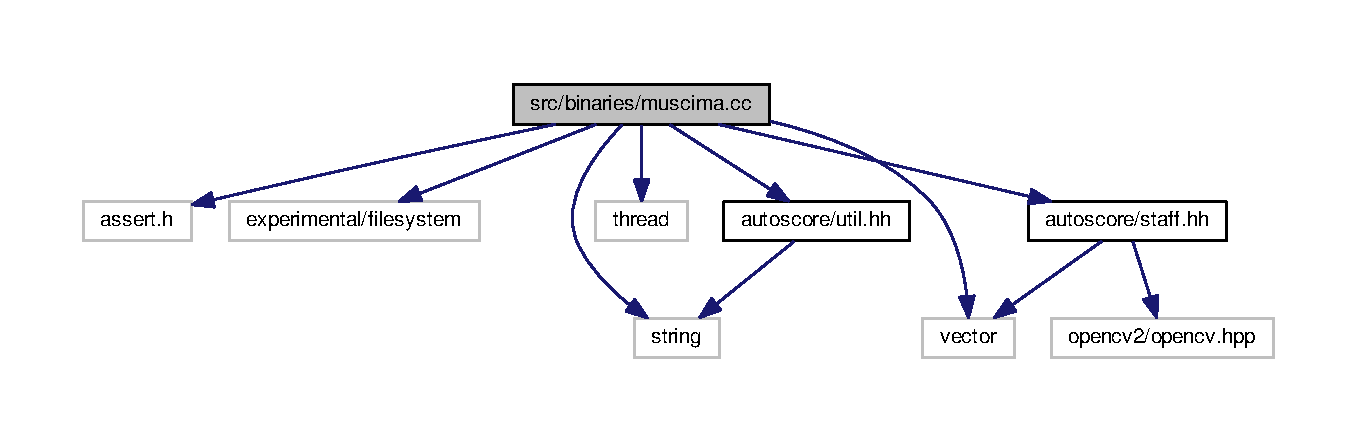
\includegraphics[width=350pt]{muscima_8cc__incl}
\end{center}
\end{figure}
\subsection*{Macros}
\begin{DoxyCompactItemize}
\item 
\#define \hyperlink{muscima_8cc_a1f08b99bca257ad31559e1eb2fce4844}{F\+N\+\_\+\+D\+A\+T\+A\+S\+ET}~\char`\"{}../datasets/Handwritten/xml\char`\"{}
\item 
\#define \hyperlink{muscima_8cc_a6d1102e5aefefff081698ae8409fc8af}{N\+\_\+\+S\+C\+O\+R\+E\+S\+\_\+\+P\+E\+R\+\_\+W}~20
\item 
\#define \hyperlink{muscima_8cc_aacd9f8bfa223a964f4b14409a229e8a4}{N\+\_\+\+W\+R\+I\+T\+E\+RS}~50
\end{DoxyCompactItemize}
\subsection*{Functions}
\begin{DoxyCompactItemize}
\item 
void \hyperlink{muscima_8cc_a5e040f7303b8f39f6cde816932e2a53c}{process\+\_\+p} (std\+::vector$<$ std\+::string $>$\+::iterator start, const int n\+\_\+files, const int writer, const std\+::string dist)
\item 
int \hyperlink{muscima_8cc_a3c04138a5bfe5d72780bb7e82a18e627}{main} (int argc, char $\ast$$\ast$argv)
\end{DoxyCompactItemize}


\subsection{Macro Definition Documentation}
\index{muscima.\+cc@{muscima.\+cc}!F\+N\+\_\+\+D\+A\+T\+A\+S\+ET@{F\+N\+\_\+\+D\+A\+T\+A\+S\+ET}}
\index{F\+N\+\_\+\+D\+A\+T\+A\+S\+ET@{F\+N\+\_\+\+D\+A\+T\+A\+S\+ET}!muscima.\+cc@{muscima.\+cc}}
\subsubsection[{\texorpdfstring{F\+N\+\_\+\+D\+A\+T\+A\+S\+ET}{FN_DATASET}}]{\setlength{\rightskip}{0pt plus 5cm}\#define F\+N\+\_\+\+D\+A\+T\+A\+S\+ET~\char`\"{}../datasets/Handwritten/xml\char`\"{}}\hypertarget{muscima_8cc_a1f08b99bca257ad31559e1eb2fce4844}{}\label{muscima_8cc_a1f08b99bca257ad31559e1eb2fce4844}


Definition at line 10 of file muscima.\+cc.

\index{muscima.\+cc@{muscima.\+cc}!N\+\_\+\+S\+C\+O\+R\+E\+S\+\_\+\+P\+E\+R\+\_\+W@{N\+\_\+\+S\+C\+O\+R\+E\+S\+\_\+\+P\+E\+R\+\_\+W}}
\index{N\+\_\+\+S\+C\+O\+R\+E\+S\+\_\+\+P\+E\+R\+\_\+W@{N\+\_\+\+S\+C\+O\+R\+E\+S\+\_\+\+P\+E\+R\+\_\+W}!muscima.\+cc@{muscima.\+cc}}
\subsubsection[{\texorpdfstring{N\+\_\+\+S\+C\+O\+R\+E\+S\+\_\+\+P\+E\+R\+\_\+W}{N_SCORES_PER_W}}]{\setlength{\rightskip}{0pt plus 5cm}\#define N\+\_\+\+S\+C\+O\+R\+E\+S\+\_\+\+P\+E\+R\+\_\+W~20}\hypertarget{muscima_8cc_a6d1102e5aefefff081698ae8409fc8af}{}\label{muscima_8cc_a6d1102e5aefefff081698ae8409fc8af}


Definition at line 11 of file muscima.\+cc.

\index{muscima.\+cc@{muscima.\+cc}!N\+\_\+\+W\+R\+I\+T\+E\+RS@{N\+\_\+\+W\+R\+I\+T\+E\+RS}}
\index{N\+\_\+\+W\+R\+I\+T\+E\+RS@{N\+\_\+\+W\+R\+I\+T\+E\+RS}!muscima.\+cc@{muscima.\+cc}}
\subsubsection[{\texorpdfstring{N\+\_\+\+W\+R\+I\+T\+E\+RS}{N_WRITERS}}]{\setlength{\rightskip}{0pt plus 5cm}\#define N\+\_\+\+W\+R\+I\+T\+E\+RS~50}\hypertarget{muscima_8cc_aacd9f8bfa223a964f4b14409a229e8a4}{}\label{muscima_8cc_aacd9f8bfa223a964f4b14409a229e8a4}


Definition at line 12 of file muscima.\+cc.



\subsection{Function Documentation}
\index{muscima.\+cc@{muscima.\+cc}!main@{main}}
\index{main@{main}!muscima.\+cc@{muscima.\+cc}}
\subsubsection[{\texorpdfstring{main(int argc, char $\ast$$\ast$argv)}{main(int argc, char **argv)}}]{\setlength{\rightskip}{0pt plus 5cm}int main (
\begin{DoxyParamCaption}
\item[{int}]{argc, }
\item[{char $\ast$$\ast$}]{argv}
\end{DoxyParamCaption}
)}\hypertarget{muscima_8cc_a3c04138a5bfe5d72780bb7e82a18e627}{}\label{muscima_8cc_a3c04138a5bfe5d72780bb7e82a18e627}


Definition at line 45 of file muscima.\+cc.

\index{muscima.\+cc@{muscima.\+cc}!process\+\_\+p@{process\+\_\+p}}
\index{process\+\_\+p@{process\+\_\+p}!muscima.\+cc@{muscima.\+cc}}
\subsubsection[{\texorpdfstring{process\+\_\+p(std\+::vector$<$ std\+::string $>$\+::iterator start, const int n\+\_\+files, const int writer, const std\+::string dist)}{process_p(std::vector< std::string >::iterator start, const int n_files, const int writer, const std::string dist)}}]{\setlength{\rightskip}{0pt plus 5cm}void process\+\_\+p (
\begin{DoxyParamCaption}
\item[{std\+::vector$<$ std\+::string $>$\+::iterator}]{start, }
\item[{const int}]{n\+\_\+files, }
\item[{const int}]{writer, }
\item[{const std\+::string}]{dist}
\end{DoxyParamCaption}
)}\hypertarget{muscima_8cc_a5e040f7303b8f39f6cde816932e2a53c}{}\label{muscima_8cc_a5e040f7303b8f39f6cde816932e2a53c}


Definition at line 17 of file muscima.\+cc.


%--- End generated contents ---

% Index
\backmatter
\newpage
\phantomsection
\clearemptydoublepage
\addcontentsline{toc}{chapter}{Index}
\printindex

\end{document}
